\PassOptionsToPackage{unicode=true}{hyperref} % options for packages loaded elsewhere
\PassOptionsToPackage{hyphens}{url}
%
\documentclass[11pt,ignorenonframetext,]{beamer}
\usepackage{pgfpages}
\setbeamertemplate{caption}[numbered]
\setbeamertemplate{caption label separator}{: }
\setbeamercolor{caption name}{fg=normal text.fg}
\beamertemplatenavigationsymbolsempty
% Prevent slide breaks in the middle of a paragraph:
\widowpenalties 1 10000
\raggedbottom
\setbeamertemplate{part page}{
\centering
\begin{beamercolorbox}[sep=16pt,center]{part title}
  \usebeamerfont{part title}\insertpart\par
\end{beamercolorbox}
}
\setbeamertemplate{section page}{
\centering
\begin{beamercolorbox}[sep=12pt,center]{part title}
  \usebeamerfont{section title}\insertsection\par
\end{beamercolorbox}
}
\setbeamertemplate{subsection page}{
\centering
\begin{beamercolorbox}[sep=8pt,center]{part title}
  \usebeamerfont{subsection title}\insertsubsection\par
\end{beamercolorbox}
}
\AtBeginPart{
  \frame{\partpage}
}
\AtBeginSection{
  \ifbibliography
  \else
    \frame{\sectionpage}
  \fi
}
\AtBeginSubsection{
  \frame{\subsectionpage}
}
\usepackage{lmodern}
\usepackage{amssymb,amsmath}
\usepackage{ifxetex,ifluatex}
\usepackage{fixltx2e} % provides \textsubscript
\ifnum 0\ifxetex 1\fi\ifluatex 1\fi=0 % if pdftex
  \usepackage[T1]{fontenc}
  \usepackage[utf8]{inputenc}
  \usepackage{textcomp} % provides euro and other symbols
\else % if luatex or xelatex
  \usepackage{unicode-math}
  \defaultfontfeatures{Ligatures=TeX,Scale=MatchLowercase}
\fi
\usetheme[]{Montpellier}
\usecolortheme{beaver}
% use upquote if available, for straight quotes in verbatim environments
\IfFileExists{upquote.sty}{\usepackage{upquote}}{}
% use microtype if available
\IfFileExists{microtype.sty}{%
\usepackage[]{microtype}
\UseMicrotypeSet[protrusion]{basicmath} % disable protrusion for tt fonts
}{}
\IfFileExists{parskip.sty}{%
\usepackage{parskip}
}{% else
\setlength{\parindent}{0pt}
\setlength{\parskip}{6pt plus 2pt minus 1pt}
}
\usepackage{hyperref}
\hypersetup{
            pdftitle={Etude des effets des pésticides dans la production des vins de table},
            pdfauthor={A. Blanc, N. Gusarov, S. Picon},
            pdfborder={0 0 0},
            breaklinks=true}
\urlstyle{same}  % don't use monospace font for urls
\newif\ifbibliography
\usepackage{graphicx,grffile}
\makeatletter
\def\maxwidth{\ifdim\Gin@nat@width>\linewidth\linewidth\else\Gin@nat@width\fi}
\def\maxheight{\ifdim\Gin@nat@height>\textheight\textheight\else\Gin@nat@height\fi}
\makeatother
% Scale images if necessary, so that they will not overflow the page
% margins by default, and it is still possible to overwrite the defaults
% using explicit options in \includegraphics[width, height, ...]{}
\setkeys{Gin}{width=\maxwidth,height=\maxheight,keepaspectratio}
\setlength{\emergencystretch}{3em}  % prevent overfull lines
\providecommand{\tightlist}{%
  \setlength{\itemsep}{0pt}\setlength{\parskip}{0pt}}
\setcounter{secnumdepth}{0}

% set default figure placement to htbp
\makeatletter
\def\fps@figure{htbp}
\makeatother

\usepackage{array}
\usepackage{multicol}

\title{Etude des effets des pésticides dans la production des vins de table}
\providecommand{\subtitle}[1]{}
\subtitle{Analyse empirique des marchés}
\author{A. Blanc, N. Gusarov, S. Picon}
\providecommand{\institute}[1]{}
\institute{Université Grenoble Alpes}
\date{11/12/2019}

\begin{document}
\frame{\titlepage}

\begin{frame}
\tableofcontents[hideallsubsections]
\end{frame}
\begin{frame}{Introduction}
\protect\hypertarget{introduction}{}

\end{frame}

\begin{frame}{Plan de la présentation}
\protect\hypertarget{plan-de-la-presentation}{}

\begin{itemize}
\tightlist
\item
  Présentation de la problématique
\item
  Présentation des données
\item
  Modélisation
\item
  Les résultats
\end{itemize}

\end{frame}

\begin{frame}{Le problème des pesticides}
\protect\hypertarget{le-probleme-des-pesticides}{}

\begin{itemize}
\tightlist
\item
  Présentation du problème des pésticides
\item
  Etat actuel
\item
  Comment combattre
\end{itemize}

\end{frame}

\begin{frame}{Le marché du vin français}
\protect\hypertarget{le-marche-du-vin-francais}{}

\begin{itemize}
\tightlist
\item
  Le marché commun
\item
  Utilisation des pésticides
\item
  Heterogénéité
\item
  Pourquoi vins de table
\end{itemize}

\end{frame}

\begin{frame}{Le Modèle théorique}
\protect\hypertarget{le-modele-theorique}{}

\begin{itemize}
\tightlist
\item
  Le rôle des pesticides dans la production du vin
\item
  Le rôle de la demande sur la production et l'offre en général
\item
  La formalisation et les équations
\end{itemize}

\end{frame}

\begin{frame}{Les données}
\protect\hypertarget{les-donnees}{}

\begin{itemize}
\tightlist
\item
  Dimentions :

  \begin{itemize}
  \tightlist
  \item
    Départements
  \item
    Années
  \end{itemize}
\item
  Les variables :

  \begin{itemize}
  \tightlist
  \item
    Pésticides (quantités)
  \item
    Vins (quantités produits, prix)
  \item
    Variables de controle (revenus, surface cultivé)
  \end{itemize}
\end{itemize}

\end{frame}

\begin{frame}{Les statistiques déscriptives}
\protect\hypertarget{les-statistiques-descriptives}{}

\begin{itemize}
\tightlist
\item
  Between and within variance par variable
\item
  Bivariate plots with support regressions
\item
  Covariance analysis
\item
  Fixed vs Random effects
\end{itemize}

\end{frame}

\begin{frame}{Etude de la variance}
\protect\hypertarget{etude-de-la-variance}{}

\tiny
\begin{table}[!htbp] \centering 
  \caption{Variance study}
\begin{tabular}{@{\extracolsep{5pt}} l|cccc} 
\\[-1.8ex]\hline 
\hline \\[-1.8ex] 
 & Mean & Overall & Between & Within \\ 
\hline \\[-1.8ex] 
Index prix & $0.175$ & $0.568$ & $0.368$ & $0.434$ \\ 
Index pesticides & $0.170$ & $0.333$ & $0.239$ & $0.234$ \\ 
Surface & $4.892$ & $1.986$ & $1.955$ & $0.410$ \\ 
Revenus & $9.891$ & $0.061$ & $0.061$ & $0.011$ \\ 
Temps & $3$ & $1.416$ & $0$ & $1.416$ \\ 
\hline \\[-1.8ex] 
\end{tabular} 
\end{table}

\end{frame}

\begin{frame}[fragile]{Visualisatoin des interdependances}
\protect\hypertarget{visualisatoin-des-interdependances}{}

\begin{verbatim}
## `geom_smooth()` using method = 'loess' and formula 'y ~ x'
\end{verbatim}

\begin{verbatim}
## Warning in simpleLoess(y, x, w, span, degree = degree, parametric =
## parametric, : span too small. fewer data values than degrees of freedom.
\end{verbatim}

\begin{verbatim}
## Warning in simpleLoess(y, x, w, span, degree = degree, parametric =
## parametric, : pseudoinverse used at 9.2573
\end{verbatim}

\begin{verbatim}
## Warning in simpleLoess(y, x, w, span, degree = degree, parametric =
## parametric, : neighborhood radius 0.18005
\end{verbatim}

\begin{verbatim}
## Warning in simpleLoess(y, x, w, span, degree = degree, parametric =
## parametric, : reciprocal condition number 0
\end{verbatim}

\begin{verbatim}
## Warning in simpleLoess(y, x, w, span, degree = degree, parametric =
## parametric, : There are other near singularities as well. 0.014865
\end{verbatim}

\begin{verbatim}
## Warning in simpleLoess(y, x, w, span, degree = degree, parametric =
## parametric, : span too small. fewer data values than degrees of freedom.
\end{verbatim}

\begin{verbatim}
## Warning in simpleLoess(y, x, w, span, degree = degree, parametric =
## parametric, : pseudoinverse used at 5.0053
\end{verbatim}

\begin{verbatim}
## Warning in simpleLoess(y, x, w, span, degree = degree, parametric =
## parametric, : neighborhood radius 0.87248
\end{verbatim}

\begin{verbatim}
## Warning in simpleLoess(y, x, w, span, degree = degree, parametric =
## parametric, : reciprocal condition number 0
\end{verbatim}

\begin{verbatim}
## Warning in simpleLoess(y, x, w, span, degree = degree, parametric =
## parametric, : There are other near singularities as well. 0.045976
\end{verbatim}

\begin{verbatim}
## Warning in simpleLoess(y, x, w, span, degree = degree, parametric =
## parametric, : Chernobyl! trL>n 5

## Warning in simpleLoess(y, x, w, span, degree = degree, parametric =
## parametric, : Chernobyl! trL>n 5
\end{verbatim}

\begin{verbatim}
## Warning in sqrt(sum.squares/one.delta): production de NaN
\end{verbatim}

\begin{verbatim}
## Warning in simpleLoess(y, x, w, span, degree = degree, parametric =
## parametric, : span too small. fewer data values than degrees of freedom.
\end{verbatim}

\begin{verbatim}
## Warning in simpleLoess(y, x, w, span, degree = degree, parametric =
## parametric, : pseudoinverse used at 7.6162
\end{verbatim}

\begin{verbatim}
## Warning in simpleLoess(y, x, w, span, degree = degree, parametric =
## parametric, : neighborhood radius 0.3144
\end{verbatim}

\begin{verbatim}
## Warning in simpleLoess(y, x, w, span, degree = degree, parametric =
## parametric, : reciprocal condition number 0
\end{verbatim}

\begin{verbatim}
## Warning in simpleLoess(y, x, w, span, degree = degree, parametric =
## parametric, : There are other near singularities as well. 0.042878
\end{verbatim}

\begin{verbatim}
## Warning in simpleLoess(y, x, w, span, degree = degree, parametric =
## parametric, : Chernobyl! trL>n 5

## Warning in simpleLoess(y, x, w, span, degree = degree, parametric =
## parametric, : Chernobyl! trL>n 5
\end{verbatim}

\begin{verbatim}
## Warning in sqrt(sum.squares/one.delta): production de NaN
\end{verbatim}

\begin{verbatim}
## Warning in simpleLoess(y, x, w, span, degree = degree, parametric =
## parametric, : span too small. fewer data values than degrees of freedom.
\end{verbatim}

\begin{verbatim}
## Warning in simpleLoess(y, x, w, span, degree = degree, parametric =
## parametric, : pseudoinverse used at 8.2028
\end{verbatim}

\begin{verbatim}
## Warning in simpleLoess(y, x, w, span, degree = degree, parametric =
## parametric, : neighborhood radius 0.27479
\end{verbatim}

\begin{verbatim}
## Warning in simpleLoess(y, x, w, span, degree = degree, parametric =
## parametric, : reciprocal condition number 0
\end{verbatim}

\begin{verbatim}
## Warning in simpleLoess(y, x, w, span, degree = degree, parametric =
## parametric, : There are other near singularities as well. 0.18404
\end{verbatim}

\begin{verbatim}
## Warning in simpleLoess(y, x, w, span, degree = degree, parametric =
## parametric, : span too small. fewer data values than degrees of freedom.
\end{verbatim}

\begin{verbatim}
## Warning in simpleLoess(y, x, w, span, degree = degree, parametric =
## parametric, : pseudoinverse used at 5.7703
\end{verbatim}

\begin{verbatim}
## Warning in simpleLoess(y, x, w, span, degree = degree, parametric =
## parametric, : neighborhood radius 0.067414
\end{verbatim}

\begin{verbatim}
## Warning in simpleLoess(y, x, w, span, degree = degree, parametric =
## parametric, : reciprocal condition number 0
\end{verbatim}

\begin{verbatim}
## Warning in simpleLoess(y, x, w, span, degree = degree, parametric =
## parametric, : There are other near singularities as well. 0.025551
\end{verbatim}

\begin{verbatim}
## Warning in simpleLoess(y, x, w, span, degree = degree, parametric =
## parametric, : Chernobyl! trL>n 5

## Warning in simpleLoess(y, x, w, span, degree = degree, parametric =
## parametric, : Chernobyl! trL>n 5
\end{verbatim}

\begin{verbatim}
## Warning in sqrt(sum.squares/one.delta): production de NaN
\end{verbatim}

\begin{verbatim}
## Warning in simpleLoess(y, x, w, span, degree = degree, parametric =
## parametric, : span too small. fewer data values than degrees of freedom.
\end{verbatim}

\begin{verbatim}
## Warning in simpleLoess(y, x, w, span, degree = degree, parametric =
## parametric, : pseudoinverse used at 4.5043
\end{verbatim}

\begin{verbatim}
## Warning in simpleLoess(y, x, w, span, degree = degree, parametric =
## parametric, : neighborhood radius 0.96381
\end{verbatim}

\begin{verbatim}
## Warning in simpleLoess(y, x, w, span, degree = degree, parametric =
## parametric, : reciprocal condition number 0
\end{verbatim}

\begin{verbatim}
## Warning in simpleLoess(y, x, w, span, degree = degree, parametric =
## parametric, : There are other near singularities as well. 0.1394
\end{verbatim}

\begin{verbatim}
## Warning in simpleLoess(y, x, w, span, degree = degree, parametric =
## parametric, : Chernobyl! trL>n 5

## Warning in simpleLoess(y, x, w, span, degree = degree, parametric =
## parametric, : Chernobyl! trL>n 5
\end{verbatim}

\begin{verbatim}
## Warning in sqrt(sum.squares/one.delta): production de NaN
\end{verbatim}

\begin{verbatim}
## Warning in simpleLoess(y, x, w, span, degree = degree, parametric =
## parametric, : span too small. fewer data values than degrees of freedom.
\end{verbatim}

\begin{verbatim}
## Warning in simpleLoess(y, x, w, span, degree = degree, parametric =
## parametric, : pseudoinverse used at 9.9129
\end{verbatim}

\begin{verbatim}
## Warning in simpleLoess(y, x, w, span, degree = degree, parametric =
## parametric, : neighborhood radius 0.20921
\end{verbatim}

\begin{verbatim}
## Warning in simpleLoess(y, x, w, span, degree = degree, parametric =
## parametric, : reciprocal condition number 0
\end{verbatim}

\begin{verbatim}
## Warning in simpleLoess(y, x, w, span, degree = degree, parametric =
## parametric, : There are other near singularities as well. 0.38525
\end{verbatim}

\begin{verbatim}
## Warning in simpleLoess(y, x, w, span, degree = degree, parametric =
## parametric, : span too small. fewer data values than degrees of freedom.
\end{verbatim}

\begin{verbatim}
## Warning in simpleLoess(y, x, w, span, degree = degree, parametric =
## parametric, : pseudoinverse used at 5.4467
\end{verbatim}

\begin{verbatim}
## Warning in simpleLoess(y, x, w, span, degree = degree, parametric =
## parametric, : neighborhood radius 0.33712
\end{verbatim}

\begin{verbatim}
## Warning in simpleLoess(y, x, w, span, degree = degree, parametric =
## parametric, : reciprocal condition number 0
\end{verbatim}

\begin{verbatim}
## Warning in simpleLoess(y, x, w, span, degree = degree, parametric =
## parametric, : There are other near singularities as well. 0.28909
\end{verbatim}

\begin{verbatim}
## Warning in simpleLoess(y, x, w, span, degree = degree, parametric =
## parametric, : span too small. fewer data values than degrees of freedom.
\end{verbatim}

\begin{verbatim}
## Warning in simpleLoess(y, x, w, span, degree = degree, parametric =
## parametric, : pseudoinverse used at 5.1268
\end{verbatim}

\begin{verbatim}
## Warning in simpleLoess(y, x, w, span, degree = degree, parametric =
## parametric, : neighborhood radius 1.5299
\end{verbatim}

\begin{verbatim}
## Warning in simpleLoess(y, x, w, span, degree = degree, parametric =
## parametric, : reciprocal condition number 0
\end{verbatim}

\begin{verbatim}
## Warning in simpleLoess(y, x, w, span, degree = degree, parametric =
## parametric, : There are other near singularities as well. 0.078834
\end{verbatim}

\begin{verbatim}
## Warning in simpleLoess(y, x, w, span, degree = degree, parametric =
## parametric, : span too small. fewer data values than degrees of freedom.
\end{verbatim}

\begin{verbatim}
## Warning in simpleLoess(y, x, w, span, degree = degree, parametric =
## parametric, : pseudoinverse used at 12.237
\end{verbatim}

\begin{verbatim}
## Warning in simpleLoess(y, x, w, span, degree = degree, parametric =
## parametric, : neighborhood radius 0.29044
\end{verbatim}

\begin{verbatim}
## Warning in simpleLoess(y, x, w, span, degree = degree, parametric =
## parametric, : reciprocal condition number 0
\end{verbatim}

\begin{verbatim}
## Warning in simpleLoess(y, x, w, span, degree = degree, parametric =
## parametric, : There are other near singularities as well. 0.096775
\end{verbatim}

\begin{verbatim}
## Warning in simpleLoess(y, x, w, span, degree = degree, parametric =
## parametric, : span too small. fewer data values than degrees of freedom.
\end{verbatim}

\begin{verbatim}
## Warning in simpleLoess(y, x, w, span, degree = degree, parametric =
## parametric, : pseudoinverse used at 7.3144
\end{verbatim}

\begin{verbatim}
## Warning in simpleLoess(y, x, w, span, degree = degree, parametric =
## parametric, : neighborhood radius 0.95279
\end{verbatim}

\begin{verbatim}
## Warning in simpleLoess(y, x, w, span, degree = degree, parametric =
## parametric, : reciprocal condition number 0
\end{verbatim}

\begin{verbatim}
## Warning in simpleLoess(y, x, w, span, degree = degree, parametric =
## parametric, : There are other near singularities as well. 0.080618
\end{verbatim}

\begin{verbatim}
## Warning in simpleLoess(y, x, w, span, degree = degree, parametric =
## parametric, : Chernobyl! trL>n 5

## Warning in simpleLoess(y, x, w, span, degree = degree, parametric =
## parametric, : Chernobyl! trL>n 5
\end{verbatim}

\begin{verbatim}
## Warning in sqrt(sum.squares/one.delta): production de NaN
\end{verbatim}

\begin{verbatim}
## Warning in simpleLoess(y, x, w, span, degree = degree, parametric =
## parametric, : span too small. fewer data values than degrees of freedom.
\end{verbatim}

\begin{verbatim}
## Warning in simpleLoess(y, x, w, span, degree = degree, parametric =
## parametric, : pseudoinverse used at 9.2547
\end{verbatim}

\begin{verbatim}
## Warning in simpleLoess(y, x, w, span, degree = degree, parametric =
## parametric, : neighborhood radius 0.27472
\end{verbatim}

\begin{verbatim}
## Warning in simpleLoess(y, x, w, span, degree = degree, parametric =
## parametric, : reciprocal condition number 0
\end{verbatim}

\begin{verbatim}
## Warning in simpleLoess(y, x, w, span, degree = degree, parametric =
## parametric, : There are other near singularities as well. 0.53273
\end{verbatim}

\begin{verbatim}
## Warning in simpleLoess(y, x, w, span, degree = degree, parametric =
## parametric, : span too small. fewer data values than degrees of freedom.
\end{verbatim}

\begin{verbatim}
## Warning in simpleLoess(y, x, w, span, degree = degree, parametric =
## parametric, : pseudoinverse used at 2.293
\end{verbatim}

\begin{verbatim}
## Warning in simpleLoess(y, x, w, span, degree = degree, parametric =
## parametric, : neighborhood radius 1.5571
\end{verbatim}

\begin{verbatim}
## Warning in simpleLoess(y, x, w, span, degree = degree, parametric =
## parametric, : reciprocal condition number 0
\end{verbatim}

\begin{verbatim}
## Warning in simpleLoess(y, x, w, span, degree = degree, parametric =
## parametric, : There are other near singularities as well. 0.15493
\end{verbatim}

\begin{verbatim}
## Warning in simpleLoess(y, x, w, span, degree = degree, parametric =
## parametric, : Chernobyl! trL>n 5

## Warning in simpleLoess(y, x, w, span, degree = degree, parametric =
## parametric, : Chernobyl! trL>n 5
\end{verbatim}

\begin{verbatim}
## Warning in sqrt(sum.squares/one.delta): production de NaN
\end{verbatim}

\begin{verbatim}
## Warning in simpleLoess(y, x, w, span, degree = degree, parametric =
## parametric, : span too small. fewer data values than degrees of freedom.
\end{verbatim}

\begin{verbatim}
## Warning in simpleLoess(y, x, w, span, degree = degree, parametric =
## parametric, : pseudoinverse used at 10.225
\end{verbatim}

\begin{verbatim}
## Warning in simpleLoess(y, x, w, span, degree = degree, parametric =
## parametric, : neighborhood radius 0.22617
\end{verbatim}

\begin{verbatim}
## Warning in simpleLoess(y, x, w, span, degree = degree, parametric =
## parametric, : reciprocal condition number 0
\end{verbatim}

\begin{verbatim}
## Warning in simpleLoess(y, x, w, span, degree = degree, parametric =
## parametric, : There are other near singularities as well. 0.23941
\end{verbatim}

\begin{verbatim}
## Warning in simpleLoess(y, x, w, span, degree = degree, parametric =
## parametric, : span too small. fewer data values than degrees of freedom.
\end{verbatim}

\begin{verbatim}
## Warning in simpleLoess(y, x, w, span, degree = degree, parametric =
## parametric, : pseudoinverse used at 10.753
\end{verbatim}

\begin{verbatim}
## Warning in simpleLoess(y, x, w, span, degree = degree, parametric =
## parametric, : neighborhood radius 0.60825
\end{verbatim}

\begin{verbatim}
## Warning in simpleLoess(y, x, w, span, degree = degree, parametric =
## parametric, : reciprocal condition number 0
\end{verbatim}

\begin{verbatim}
## Warning in simpleLoess(y, x, w, span, degree = degree, parametric =
## parametric, : There are other near singularities as well. 0.099223
\end{verbatim}

\begin{verbatim}
## Warning in simpleLoess(y, x, w, span, degree = degree, parametric =
## parametric, : span too small. fewer data values than degrees of freedom.
\end{verbatim}

\begin{verbatim}
## Warning in simpleLoess(y, x, w, span, degree = degree, parametric =
## parametric, : pseudoinverse used at 6.4843
\end{verbatim}

\begin{verbatim}
## Warning in simpleLoess(y, x, w, span, degree = degree, parametric =
## parametric, : neighborhood radius 1.1495
\end{verbatim}

\begin{verbatim}
## Warning in simpleLoess(y, x, w, span, degree = degree, parametric =
## parametric, : reciprocal condition number 0
\end{verbatim}

\begin{verbatim}
## Warning in simpleLoess(y, x, w, span, degree = degree, parametric =
## parametric, : There are other near singularities as well. 0.019423
\end{verbatim}

\begin{verbatim}
## Warning in simpleLoess(y, x, w, span, degree = degree, parametric =
## parametric, : span too small. fewer data values than degrees of freedom.
\end{verbatim}

\begin{verbatim}
## Warning in simpleLoess(y, x, w, span, degree = degree, parametric =
## parametric, : pseudoinverse used at 6.9468
\end{verbatim}

\begin{verbatim}
## Warning in simpleLoess(y, x, w, span, degree = degree, parametric =
## parametric, : neighborhood radius 0.41839
\end{verbatim}

\begin{verbatim}
## Warning in simpleLoess(y, x, w, span, degree = degree, parametric =
## parametric, : reciprocal condition number 0
\end{verbatim}

\begin{verbatim}
## Warning in simpleLoess(y, x, w, span, degree = degree, parametric =
## parametric, : There are other near singularities as well. 0.34638
\end{verbatim}

\begin{verbatim}
## Warning in simpleLoess(y, x, w, span, degree = degree, parametric =
## parametric, : span too small. fewer data values than degrees of freedom.
\end{verbatim}

\begin{verbatim}
## Warning in simpleLoess(y, x, w, span, degree = degree, parametric =
## parametric, : pseudoinverse used at 6.5674
\end{verbatim}

\begin{verbatim}
## Warning in simpleLoess(y, x, w, span, degree = degree, parametric =
## parametric, : neighborhood radius 0.83082
\end{verbatim}

\begin{verbatim}
## Warning in simpleLoess(y, x, w, span, degree = degree, parametric =
## parametric, : reciprocal condition number 0
\end{verbatim}

\begin{verbatim}
## Warning in simpleLoess(y, x, w, span, degree = degree, parametric =
## parametric, : There are other near singularities as well. 0.53223
\end{verbatim}

\begin{verbatim}
## Warning in simpleLoess(y, x, w, span, degree = degree, parametric =
## parametric, : span too small. fewer data values than degrees of freedom.
\end{verbatim}

\begin{verbatim}
## Warning in simpleLoess(y, x, w, span, degree = degree, parametric =
## parametric, : pseudoinverse used at 9.5597
\end{verbatim}

\begin{verbatim}
## Warning in simpleLoess(y, x, w, span, degree = degree, parametric =
## parametric, : neighborhood radius 0.41892
\end{verbatim}

\begin{verbatim}
## Warning in simpleLoess(y, x, w, span, degree = degree, parametric =
## parametric, : reciprocal condition number 0
\end{verbatim}

\begin{verbatim}
## Warning in simpleLoess(y, x, w, span, degree = degree, parametric =
## parametric, : There are other near singularities as well. 0.68519
\end{verbatim}

\begin{verbatim}
## Warning in simpleLoess(y, x, w, span, degree = degree, parametric =
## parametric, : span too small. fewer data values than degrees of freedom.
\end{verbatim}

\begin{verbatim}
## Warning in simpleLoess(y, x, w, span, degree = degree, parametric =
## parametric, : pseudoinverse used at 5.9933
\end{verbatim}

\begin{verbatim}
## Warning in simpleLoess(y, x, w, span, degree = degree, parametric =
## parametric, : neighborhood radius 0.12696
\end{verbatim}

\begin{verbatim}
## Warning in simpleLoess(y, x, w, span, degree = degree, parametric =
## parametric, : reciprocal condition number 0
\end{verbatim}

\begin{verbatim}
## Warning in simpleLoess(y, x, w, span, degree = degree, parametric =
## parametric, : There are other near singularities as well. 1.0066
\end{verbatim}

\begin{verbatim}
## Warning in simpleLoess(y, x, w, span, degree = degree, parametric =
## parametric, : span too small. fewer data values than degrees of freedom.
\end{verbatim}

\begin{verbatim}
## Warning in simpleLoess(y, x, w, span, degree = degree, parametric =
## parametric, : pseudoinverse used at 8.5536
\end{verbatim}

\begin{verbatim}
## Warning in simpleLoess(y, x, w, span, degree = degree, parametric =
## parametric, : neighborhood radius 0.60138
\end{verbatim}

\begin{verbatim}
## Warning in simpleLoess(y, x, w, span, degree = degree, parametric =
## parametric, : reciprocal condition number 0
\end{verbatim}

\begin{verbatim}
## Warning in simpleLoess(y, x, w, span, degree = degree, parametric =
## parametric, : There are other near singularities as well. 0.45536
\end{verbatim}

\begin{verbatim}
## Warning in simpleLoess(y, x, w, span, degree = degree, parametric =
## parametric, : span too small. fewer data values than degrees of freedom.
\end{verbatim}

\begin{verbatim}
## Warning in simpleLoess(y, x, w, span, degree = degree, parametric =
## parametric, : pseudoinverse used at 12.252
\end{verbatim}

\begin{verbatim}
## Warning in simpleLoess(y, x, w, span, degree = degree, parametric =
## parametric, : neighborhood radius 0.19328
\end{verbatim}

\begin{verbatim}
## Warning in simpleLoess(y, x, w, span, degree = degree, parametric =
## parametric, : reciprocal condition number 0
\end{verbatim}

\begin{verbatim}
## Warning in simpleLoess(y, x, w, span, degree = degree, parametric =
## parametric, : There are other near singularities as well. 0.050849
\end{verbatim}

\begin{verbatim}
## Warning in simpleLoess(y, x, w, span, degree = degree, parametric =
## parametric, : span too small. fewer data values than degrees of freedom.
\end{verbatim}

\begin{verbatim}
## Warning in simpleLoess(y, x, w, span, degree = degree, parametric =
## parametric, : pseudoinverse used at 8.247
\end{verbatim}

\begin{verbatim}
## Warning in simpleLoess(y, x, w, span, degree = degree, parametric =
## parametric, : neighborhood radius 0.36587
\end{verbatim}

\begin{verbatim}
## Warning in simpleLoess(y, x, w, span, degree = degree, parametric =
## parametric, : reciprocal condition number 0
\end{verbatim}

\begin{verbatim}
## Warning in simpleLoess(y, x, w, span, degree = degree, parametric =
## parametric, : There are other near singularities as well. 0.17566
\end{verbatim}

\begin{verbatim}
## Warning in simpleLoess(y, x, w, span, degree = degree, parametric =
## parametric, : span too small. fewer data values than degrees of freedom.
\end{verbatim}

\begin{verbatim}
## Warning in simpleLoess(y, x, w, span, degree = degree, parametric =
## parametric, : pseudoinverse used at 11.86
\end{verbatim}

\begin{verbatim}
## Warning in simpleLoess(y, x, w, span, degree = degree, parametric =
## parametric, : neighborhood radius 0.9666
\end{verbatim}

\begin{verbatim}
## Warning in simpleLoess(y, x, w, span, degree = degree, parametric =
## parametric, : reciprocal condition number 0
\end{verbatim}

\begin{verbatim}
## Warning in simpleLoess(y, x, w, span, degree = degree, parametric =
## parametric, : There are other near singularities as well. 0.13913
\end{verbatim}

\begin{verbatim}
## Warning in simpleLoess(y, x, w, span, degree = degree, parametric =
## parametric, : span too small. fewer data values than degrees of freedom.
\end{verbatim}

\begin{verbatim}
## Warning in simpleLoess(y, x, w, span, degree = degree, parametric =
## parametric, : pseudoinverse used at 10.706
\end{verbatim}

\begin{verbatim}
## Warning in simpleLoess(y, x, w, span, degree = degree, parametric =
## parametric, : neighborhood radius 1.1776
\end{verbatim}

\begin{verbatim}
## Warning in simpleLoess(y, x, w, span, degree = degree, parametric =
## parametric, : reciprocal condition number 0
\end{verbatim}

\begin{verbatim}
## Warning in simpleLoess(y, x, w, span, degree = degree, parametric =
## parametric, : There are other near singularities as well. 0.44166
\end{verbatim}

\begin{verbatim}
## Warning in simpleLoess(y, x, w, span, degree = degree, parametric =
## parametric, : span too small. fewer data values than degrees of freedom.
\end{verbatim}

\begin{verbatim}
## Warning in simpleLoess(y, x, w, span, degree = degree, parametric =
## parametric, : pseudoinverse used at 12.633
\end{verbatim}

\begin{verbatim}
## Warning in simpleLoess(y, x, w, span, degree = degree, parametric =
## parametric, : neighborhood radius 0.35048
\end{verbatim}

\begin{verbatim}
## Warning in simpleLoess(y, x, w, span, degree = degree, parametric =
## parametric, : reciprocal condition number 0
\end{verbatim}

\begin{verbatim}
## Warning in simpleLoess(y, x, w, span, degree = degree, parametric =
## parametric, : There are other near singularities as well. 0.42041
\end{verbatim}

\begin{verbatim}
## Warning in simpleLoess(y, x, w, span, degree = degree, parametric =
## parametric, : Chernobyl! trL>n 5

## Warning in simpleLoess(y, x, w, span, degree = degree, parametric =
## parametric, : Chernobyl! trL>n 5
\end{verbatim}

\begin{verbatim}
## Warning in sqrt(sum.squares/one.delta): production de NaN
\end{verbatim}

\begin{verbatim}
## Warning in simpleLoess(y, x, w, span, degree = degree, parametric =
## parametric, : span too small. fewer data values than degrees of freedom.
\end{verbatim}

\begin{verbatim}
## Warning in simpleLoess(y, x, w, span, degree = degree, parametric =
## parametric, : pseudoinverse used at 7.9104
\end{verbatim}

\begin{verbatim}
## Warning in simpleLoess(y, x, w, span, degree = degree, parametric =
## parametric, : neighborhood radius 0.46314
\end{verbatim}

\begin{verbatim}
## Warning in simpleLoess(y, x, w, span, degree = degree, parametric =
## parametric, : reciprocal condition number 0
\end{verbatim}

\begin{verbatim}
## Warning in simpleLoess(y, x, w, span, degree = degree, parametric =
## parametric, : There are other near singularities as well. 0.1493
\end{verbatim}

\begin{verbatim}
## Warning in simpleLoess(y, x, w, span, degree = degree, parametric =
## parametric, : Chernobyl! trL>n 5

## Warning in simpleLoess(y, x, w, span, degree = degree, parametric =
## parametric, : Chernobyl! trL>n 5
\end{verbatim}

\begin{verbatim}
## Warning in sqrt(sum.squares/one.delta): production de NaN
\end{verbatim}

\begin{verbatim}
## Warning in simpleLoess(y, x, w, span, degree = degree, parametric =
## parametric, : span too small. fewer data values than degrees of freedom.
\end{verbatim}

\begin{verbatim}
## Warning in simpleLoess(y, x, w, span, degree = degree, parametric =
## parametric, : pseudoinverse used at 9.7808
\end{verbatim}

\begin{verbatim}
## Warning in simpleLoess(y, x, w, span, degree = degree, parametric =
## parametric, : neighborhood radius 0.44022
\end{verbatim}

\begin{verbatim}
## Warning in simpleLoess(y, x, w, span, degree = degree, parametric =
## parametric, : reciprocal condition number 0
\end{verbatim}

\begin{verbatim}
## Warning in simpleLoess(y, x, w, span, degree = degree, parametric =
## parametric, : There are other near singularities as well. 0.0060322
\end{verbatim}

\begin{verbatim}
## Warning in simpleLoess(y, x, w, span, degree = degree, parametric =
## parametric, : span too small. fewer data values than degrees of freedom.
\end{verbatim}

\begin{verbatim}
## Warning in simpleLoess(y, x, w, span, degree = degree, parametric =
## parametric, : pseudoinverse used at 8.5771
\end{verbatim}

\begin{verbatim}
## Warning in simpleLoess(y, x, w, span, degree = degree, parametric =
## parametric, : neighborhood radius 0.25238
\end{verbatim}

\begin{verbatim}
## Warning in simpleLoess(y, x, w, span, degree = degree, parametric =
## parametric, : reciprocal condition number 0
\end{verbatim}

\begin{verbatim}
## Warning in simpleLoess(y, x, w, span, degree = degree, parametric =
## parametric, : There are other near singularities as well. 0.080334
\end{verbatim}

\begin{verbatim}
## Warning in simpleLoess(y, x, w, span, degree = degree, parametric =
## parametric, : span too small. fewer data values than degrees of freedom.
\end{verbatim}

\begin{verbatim}
## Warning in simpleLoess(y, x, w, span, degree = degree, parametric =
## parametric, : pseudoinverse used at 8.1538
\end{verbatim}

\begin{verbatim}
## Warning in simpleLoess(y, x, w, span, degree = degree, parametric =
## parametric, : neighborhood radius 0.23551
\end{verbatim}

\begin{verbatim}
## Warning in simpleLoess(y, x, w, span, degree = degree, parametric =
## parametric, : reciprocal condition number 0
\end{verbatim}

\begin{verbatim}
## Warning in simpleLoess(y, x, w, span, degree = degree, parametric =
## parametric, : There are other near singularities as well. 0.12959
\end{verbatim}

\begin{verbatim}
## Warning in simpleLoess(y, x, w, span, degree = degree, parametric =
## parametric, : span too small. fewer data values than degrees of freedom.
\end{verbatim}

\begin{verbatim}
## Warning in simpleLoess(y, x, w, span, degree = degree, parametric =
## parametric, : pseudoinverse used at 9.0761
\end{verbatim}

\begin{verbatim}
## Warning in simpleLoess(y, x, w, span, degree = degree, parametric =
## parametric, : neighborhood radius 0.83298
\end{verbatim}

\begin{verbatim}
## Warning in simpleLoess(y, x, w, span, degree = degree, parametric =
## parametric, : reciprocal condition number 0
\end{verbatim}

\begin{verbatim}
## Warning in simpleLoess(y, x, w, span, degree = degree, parametric =
## parametric, : There are other near singularities as well. 0.43365
\end{verbatim}

\begin{verbatim}
## Warning in simpleLoess(y, x, w, span, degree = degree, parametric =
## parametric, : Chernobyl! trL>n 5

## Warning in simpleLoess(y, x, w, span, degree = degree, parametric =
## parametric, : Chernobyl! trL>n 5
\end{verbatim}

\begin{verbatim}
## Warning in sqrt(sum.squares/one.delta): production de NaN
\end{verbatim}

\begin{verbatim}
## Warning in simpleLoess(y, x, w, span, degree = degree, parametric =
## parametric, : span too small. fewer data values than degrees of freedom.
\end{verbatim}

\begin{verbatim}
## Warning in simpleLoess(y, x, w, span, degree = degree, parametric =
## parametric, : pseudoinverse used at 9.8022
\end{verbatim}

\begin{verbatim}
## Warning in simpleLoess(y, x, w, span, degree = degree, parametric =
## parametric, : neighborhood radius 0.059584
\end{verbatim}

\begin{verbatim}
## Warning in simpleLoess(y, x, w, span, degree = degree, parametric =
## parametric, : reciprocal condition number 0
\end{verbatim}

\begin{verbatim}
## Warning in simpleLoess(y, x, w, span, degree = degree, parametric =
## parametric, : There are other near singularities as well. 0.31545
\end{verbatim}

\begin{verbatim}
## Warning in simpleLoess(y, x, w, span, degree = degree, parametric =
## parametric, : span too small. fewer data values than degrees of freedom.
\end{verbatim}

\begin{verbatim}
## Warning in simpleLoess(y, x, w, span, degree = degree, parametric =
## parametric, : pseudoinverse used at 8.3937
\end{verbatim}

\begin{verbatim}
## Warning in simpleLoess(y, x, w, span, degree = degree, parametric =
## parametric, : neighborhood radius 0.39964
\end{verbatim}

\begin{verbatim}
## Warning in simpleLoess(y, x, w, span, degree = degree, parametric =
## parametric, : reciprocal condition number 0
\end{verbatim}

\begin{verbatim}
## Warning in simpleLoess(y, x, w, span, degree = degree, parametric =
## parametric, : There are other near singularities as well. 0.037518
\end{verbatim}

\begin{verbatim}
## Warning in simpleLoess(y, x, w, span, degree = degree, parametric =
## parametric, : Chernobyl! trL>n 5

## Warning in simpleLoess(y, x, w, span, degree = degree, parametric =
## parametric, : Chernobyl! trL>n 5
\end{verbatim}

\begin{verbatim}
## Warning in sqrt(sum.squares/one.delta): production de NaN
\end{verbatim}

\begin{verbatim}
## Warning in simpleLoess(y, x, w, span, degree = degree, parametric =
## parametric, : span too small. fewer data values than degrees of freedom.
\end{verbatim}

\begin{verbatim}
## Warning in simpleLoess(y, x, w, span, degree = degree, parametric =
## parametric, : pseudoinverse used at 5.0238
\end{verbatim}

\begin{verbatim}
## Warning in simpleLoess(y, x, w, span, degree = degree, parametric =
## parametric, : neighborhood radius 1.2898
\end{verbatim}

\begin{verbatim}
## Warning in simpleLoess(y, x, w, span, degree = degree, parametric =
## parametric, : reciprocal condition number 0
\end{verbatim}

\begin{verbatim}
## Warning in simpleLoess(y, x, w, span, degree = degree, parametric =
## parametric, : There are other near singularities as well. 0.0033494
\end{verbatim}

\begin{verbatim}
## Warning in simpleLoess(y, x, w, span, degree = degree, parametric =
## parametric, : span too small. fewer data values than degrees of freedom.
\end{verbatim}

\begin{verbatim}
## Warning in simpleLoess(y, x, w, span, degree = degree, parametric =
## parametric, : pseudoinverse used at 10.822
\end{verbatim}

\begin{verbatim}
## Warning in simpleLoess(y, x, w, span, degree = degree, parametric =
## parametric, : neighborhood radius 0.53267
\end{verbatim}

\begin{verbatim}
## Warning in simpleLoess(y, x, w, span, degree = degree, parametric =
## parametric, : reciprocal condition number 0
\end{verbatim}

\begin{verbatim}
## Warning in simpleLoess(y, x, w, span, degree = degree, parametric =
## parametric, : There are other near singularities as well. 0.28123
\end{verbatim}

\begin{verbatim}
## Warning in simpleLoess(y, x, w, span, degree = degree, parametric =
## parametric, : Chernobyl! trL>n 5

## Warning in simpleLoess(y, x, w, span, degree = degree, parametric =
## parametric, : Chernobyl! trL>n 5
\end{verbatim}

\begin{verbatim}
## Warning in sqrt(sum.squares/one.delta): production de NaN
\end{verbatim}

\begin{verbatim}
## Warning in simpleLoess(y, x, w, span, degree = degree, parametric =
## parametric, : span too small. fewer data values than degrees of freedom.
\end{verbatim}

\begin{verbatim}
## Warning in simpleLoess(y, x, w, span, degree = degree, parametric =
## parametric, : pseudoinverse used at 5.4583
\end{verbatim}

\begin{verbatim}
## Warning in simpleLoess(y, x, w, span, degree = degree, parametric =
## parametric, : neighborhood radius 0.69866
\end{verbatim}

\begin{verbatim}
## Warning in simpleLoess(y, x, w, span, degree = degree, parametric =
## parametric, : reciprocal condition number 0
\end{verbatim}

\begin{verbatim}
## Warning in simpleLoess(y, x, w, span, degree = degree, parametric =
## parametric, : There are other near singularities as well. 0.1724
\end{verbatim}

\begin{verbatim}
## Warning in simpleLoess(y, x, w, span, degree = degree, parametric =
## parametric, : span too small. fewer data values than degrees of freedom.
\end{verbatim}

\begin{verbatim}
## Warning in simpleLoess(y, x, w, span, degree = degree, parametric =
## parametric, : pseudoinverse used at 9.4008
\end{verbatim}

\begin{verbatim}
## Warning in simpleLoess(y, x, w, span, degree = degree, parametric =
## parametric, : neighborhood radius 0.84815
\end{verbatim}

\begin{verbatim}
## Warning in simpleLoess(y, x, w, span, degree = degree, parametric =
## parametric, : reciprocal condition number 0
\end{verbatim}

\begin{verbatim}
## Warning in simpleLoess(y, x, w, span, degree = degree, parametric =
## parametric, : There are other near singularities as well. 0.28886
\end{verbatim}

\begin{verbatim}
## Warning in simpleLoess(y, x, w, span, degree = degree, parametric =
## parametric, : span too small. fewer data values than degrees of freedom.
\end{verbatim}

\begin{verbatim}
## Warning in simpleLoess(y, x, w, span, degree = degree, parametric =
## parametric, : pseudoinverse used at 9.9168
\end{verbatim}

\begin{verbatim}
## Warning in simpleLoess(y, x, w, span, degree = degree, parametric =
## parametric, : neighborhood radius 0.75055
\end{verbatim}

\begin{verbatim}
## Warning in simpleLoess(y, x, w, span, degree = degree, parametric =
## parametric, : reciprocal condition number 0
\end{verbatim}

\begin{verbatim}
## Warning in simpleLoess(y, x, w, span, degree = degree, parametric =
## parametric, : There are other near singularities as well. 0.1819
\end{verbatim}

\begin{verbatim}
## Warning in simpleLoess(y, x, w, span, degree = degree, parametric =
## parametric, : span too small. fewer data values than degrees of freedom.
\end{verbatim}

\begin{verbatim}
## Warning in simpleLoess(y, x, w, span, degree = degree, parametric =
## parametric, : pseudoinverse used at 10.435
\end{verbatim}

\begin{verbatim}
## Warning in simpleLoess(y, x, w, span, degree = degree, parametric =
## parametric, : neighborhood radius 0.37465
\end{verbatim}

\begin{verbatim}
## Warning in simpleLoess(y, x, w, span, degree = degree, parametric =
## parametric, : reciprocal condition number 0
\end{verbatim}

\begin{verbatim}
## Warning in simpleLoess(y, x, w, span, degree = degree, parametric =
## parametric, : There are other near singularities as well. 0.0089543
\end{verbatim}

\begin{verbatim}
## Warning in simpleLoess(y, x, w, span, degree = degree, parametric =
## parametric, : span too small. fewer data values than degrees of freedom.
\end{verbatim}

\begin{verbatim}
## Warning in simpleLoess(y, x, w, span, degree = degree, parametric =
## parametric, : pseudoinverse used at 2.933
\end{verbatim}

\begin{verbatim}
## Warning in simpleLoess(y, x, w, span, degree = degree, parametric =
## parametric, : neighborhood radius 1.9191
\end{verbatim}

\begin{verbatim}
## Warning in simpleLoess(y, x, w, span, degree = degree, parametric =
## parametric, : reciprocal condition number 0
\end{verbatim}

\begin{verbatim}
## Warning in simpleLoess(y, x, w, span, degree = degree, parametric =
## parametric, : There are other near singularities as well. 0.16956
\end{verbatim}

\begin{verbatim}
## Warning in simpleLoess(y, x, w, span, degree = degree, parametric =
## parametric, : Chernobyl! trL>n 5

## Warning in simpleLoess(y, x, w, span, degree = degree, parametric =
## parametric, : Chernobyl! trL>n 5
\end{verbatim}

\begin{verbatim}
## Warning in sqrt(sum.squares/one.delta): production de NaN
\end{verbatim}

\begin{verbatim}
## Warning in simpleLoess(y, x, w, span, degree = degree, parametric =
## parametric, : span too small. fewer data values than degrees of freedom.
\end{verbatim}

\begin{verbatim}
## Warning in simpleLoess(y, x, w, span, degree = degree, parametric =
## parametric, : pseudoinverse used at 6.3397
\end{verbatim}

\begin{verbatim}
## Warning in simpleLoess(y, x, w, span, degree = degree, parametric =
## parametric, : neighborhood radius 0.24095
\end{verbatim}

\begin{verbatim}
## Warning in simpleLoess(y, x, w, span, degree = degree, parametric =
## parametric, : reciprocal condition number 0
\end{verbatim}

\begin{verbatim}
## Warning in simpleLoess(y, x, w, span, degree = degree, parametric =
## parametric, : There are other near singularities as well. 0.3662
\end{verbatim}

\begin{verbatim}
## Warning in simpleLoess(y, x, w, span, degree = degree, parametric =
## parametric, : span too small. fewer data values than degrees of freedom.
\end{verbatim}

\begin{verbatim}
## Warning in simpleLoess(y, x, w, span, degree = degree, parametric =
## parametric, : pseudoinverse used at 3.4292
\end{verbatim}

\begin{verbatim}
## Warning in simpleLoess(y, x, w, span, degree = degree, parametric =
## parametric, : neighborhood radius 0.79031
\end{verbatim}

\begin{verbatim}
## Warning in simpleLoess(y, x, w, span, degree = degree, parametric =
## parametric, : reciprocal condition number 0
\end{verbatim}

\begin{verbatim}
## Warning in simpleLoess(y, x, w, span, degree = degree, parametric =
## parametric, : There are other near singularities as well. 0.032307
\end{verbatim}

\begin{verbatim}
## Warning in simpleLoess(y, x, w, span, degree = degree, parametric =
## parametric, : span too small. fewer data values than degrees of freedom.
\end{verbatim}

\begin{verbatim}
## Warning in simpleLoess(y, x, w, span, degree = degree, parametric =
## parametric, : pseudoinverse used at 6.7945
\end{verbatim}

\begin{verbatim}
## Warning in simpleLoess(y, x, w, span, degree = degree, parametric =
## parametric, : neighborhood radius 0.52667
\end{verbatim}

\begin{verbatim}
## Warning in simpleLoess(y, x, w, span, degree = degree, parametric =
## parametric, : reciprocal condition number 0
\end{verbatim}

\begin{verbatim}
## Warning in simpleLoess(y, x, w, span, degree = degree, parametric =
## parametric, : There are other near singularities as well. 0.027384
\end{verbatim}

\begin{verbatim}
## Warning in simpleLoess(y, x, w, span, degree = degree, parametric =
## parametric, : Chernobyl! trL>n 5

## Warning in simpleLoess(y, x, w, span, degree = degree, parametric =
## parametric, : Chernobyl! trL>n 5
\end{verbatim}

\begin{verbatim}
## Warning in sqrt(sum.squares/one.delta): production de NaN
\end{verbatim}

\begin{verbatim}
## Warning in simpleLoess(y, x, w, span, degree = degree, parametric =
## parametric, : span too small. fewer data values than degrees of freedom.
\end{verbatim}

\begin{verbatim}
## Warning in simpleLoess(y, x, w, span, degree = degree, parametric =
## parametric, : pseudoinverse used at 5.3898
\end{verbatim}

\begin{verbatim}
## Warning in simpleLoess(y, x, w, span, degree = degree, parametric =
## parametric, : neighborhood radius 0.56865
\end{verbatim}

\begin{verbatim}
## Warning in simpleLoess(y, x, w, span, degree = degree, parametric =
## parametric, : reciprocal condition number 0
\end{verbatim}

\begin{verbatim}
## Warning in simpleLoess(y, x, w, span, degree = degree, parametric =
## parametric, : There are other near singularities as well. 0.044458
\end{verbatim}

\begin{verbatim}
## Warning in simpleLoess(y, x, w, span, degree = degree, parametric =
## parametric, : span too small. fewer data values than degrees of freedom.
\end{verbatim}

\begin{verbatim}
## Warning in simpleLoess(y, x, w, span, degree = degree, parametric =
## parametric, : pseudoinverse used at 5.4638
\end{verbatim}

\begin{verbatim}
## Warning in simpleLoess(y, x, w, span, degree = degree, parametric =
## parametric, : neighborhood radius 1.8613
\end{verbatim}

\begin{verbatim}
## Warning in simpleLoess(y, x, w, span, degree = degree, parametric =
## parametric, : reciprocal condition number 0
\end{verbatim}

\begin{verbatim}
## Warning in simpleLoess(y, x, w, span, degree = degree, parametric =
## parametric, : There are other near singularities as well. 0.48424
\end{verbatim}

\begin{verbatim}
## Warning in simpleLoess(y, x, w, span, degree = degree, parametric =
## parametric, : span too small. fewer data values than degrees of freedom.
\end{verbatim}

\begin{verbatim}
## Warning in simpleLoess(y, x, w, span, degree = degree, parametric =
## parametric, : pseudoinverse used at 5.7667
\end{verbatim}

\begin{verbatim}
## Warning in simpleLoess(y, x, w, span, degree = degree, parametric =
## parametric, : neighborhood radius 1.4157
\end{verbatim}

\begin{verbatim}
## Warning in simpleLoess(y, x, w, span, degree = degree, parametric =
## parametric, : reciprocal condition number 0
\end{verbatim}

\begin{verbatim}
## Warning in simpleLoess(y, x, w, span, degree = degree, parametric =
## parametric, : There are other near singularities as well. 0.030991
\end{verbatim}

\begin{verbatim}
## Warning in simpleLoess(y, x, w, span, degree = degree, parametric =
## parametric, : span too small. fewer data values than degrees of freedom.
\end{verbatim}

\begin{verbatim}
## Warning in simpleLoess(y, x, w, span, degree = degree, parametric =
## parametric, : pseudoinverse used at 1.0855
\end{verbatim}

\begin{verbatim}
## Warning in simpleLoess(y, x, w, span, degree = degree, parametric =
## parametric, : neighborhood radius 2.4699
\end{verbatim}

\begin{verbatim}
## Warning in simpleLoess(y, x, w, span, degree = degree, parametric =
## parametric, : reciprocal condition number 0
\end{verbatim}

\begin{verbatim}
## Warning in simpleLoess(y, x, w, span, degree = degree, parametric =
## parametric, : There are other near singularities as well. 0.058691
\end{verbatim}

\begin{verbatim}
## Warning in simpleLoess(y, x, w, span, degree = degree, parametric =
## parametric, : span too small. fewer data values than degrees of freedom.
\end{verbatim}

\begin{verbatim}
## Warning in simpleLoess(y, x, w, span, degree = degree, parametric =
## parametric, : pseudoinverse used at 7.755
\end{verbatim}

\begin{verbatim}
## Warning in simpleLoess(y, x, w, span, degree = degree, parametric =
## parametric, : neighborhood radius 0.74808
\end{verbatim}

\begin{verbatim}
## Warning in simpleLoess(y, x, w, span, degree = degree, parametric =
## parametric, : reciprocal condition number 0
\end{verbatim}

\begin{verbatim}
## Warning in simpleLoess(y, x, w, span, degree = degree, parametric =
## parametric, : There are other near singularities as well. 0.033004
\end{verbatim}

\begin{verbatim}
## Warning in simpleLoess(y, x, w, span, degree = degree, parametric =
## parametric, : Chernobyl! trL>n 5

## Warning in simpleLoess(y, x, w, span, degree = degree, parametric =
## parametric, : Chernobyl! trL>n 5
\end{verbatim}

\begin{verbatim}
## Warning in sqrt(sum.squares/one.delta): production de NaN
\end{verbatim}

\begin{verbatim}
## Warning in simpleLoess(y, x, w, span, degree = degree, parametric =
## parametric, : span too small. fewer data values than degrees of freedom.
\end{verbatim}

\begin{verbatim}
## Warning in simpleLoess(y, x, w, span, degree = degree, parametric =
## parametric, : pseudoinverse used at 7.7498
\end{verbatim}

\begin{verbatim}
## Warning in simpleLoess(y, x, w, span, degree = degree, parametric =
## parametric, : neighborhood radius 0.46006
\end{verbatim}

\begin{verbatim}
## Warning in simpleLoess(y, x, w, span, degree = degree, parametric =
## parametric, : reciprocal condition number 0
\end{verbatim}

\begin{verbatim}
## Warning in simpleLoess(y, x, w, span, degree = degree, parametric =
## parametric, : There are other near singularities as well. 0.098702
\end{verbatim}

\begin{verbatim}
## Warning in simpleLoess(y, x, w, span, degree = degree, parametric =
## parametric, : span too small. fewer data values than degrees of freedom.
\end{verbatim}

\begin{verbatim}
## Warning in simpleLoess(y, x, w, span, degree = degree, parametric =
## parametric, : pseudoinverse used at 6.4628
\end{verbatim}

\begin{verbatim}
## Warning in simpleLoess(y, x, w, span, degree = degree, parametric =
## parametric, : neighborhood radius 1.1169
\end{verbatim}

\begin{verbatim}
## Warning in simpleLoess(y, x, w, span, degree = degree, parametric =
## parametric, : reciprocal condition number 0
\end{verbatim}

\begin{verbatim}
## Warning in simpleLoess(y, x, w, span, degree = degree, parametric =
## parametric, : There are other near singularities as well. 0.24578
\end{verbatim}

\begin{verbatim}
## Warning in simpleLoess(y, x, w, span, degree = degree, parametric =
## parametric, : span too small. fewer data values than degrees of freedom.
\end{verbatim}

\begin{verbatim}
## Warning in simpleLoess(y, x, w, span, degree = degree, parametric =
## parametric, : pseudoinverse used at 9.581
\end{verbatim}

\begin{verbatim}
## Warning in simpleLoess(y, x, w, span, degree = degree, parametric =
## parametric, : neighborhood radius 1.0063
\end{verbatim}

\begin{verbatim}
## Warning in simpleLoess(y, x, w, span, degree = degree, parametric =
## parametric, : reciprocal condition number 0
\end{verbatim}

\begin{verbatim}
## Warning in simpleLoess(y, x, w, span, degree = degree, parametric =
## parametric, : There are other near singularities as well. 0.041869
\end{verbatim}

\begin{verbatim}
## Warning in simpleLoess(y, x, w, span, degree = degree, parametric =
## parametric, : span too small. fewer data values than degrees of freedom.
\end{verbatim}

\begin{verbatim}
## Warning in simpleLoess(y, x, w, span, degree = degree, parametric =
## parametric, : pseudoinverse used at 6.6871
\end{verbatim}

\begin{verbatim}
## Warning in simpleLoess(y, x, w, span, degree = degree, parametric =
## parametric, : neighborhood radius 1.0717
\end{verbatim}

\begin{verbatim}
## Warning in simpleLoess(y, x, w, span, degree = degree, parametric =
## parametric, : reciprocal condition number 0
\end{verbatim}

\begin{verbatim}
## Warning in simpleLoess(y, x, w, span, degree = degree, parametric =
## parametric, : There are other near singularities as well. 0.035636
\end{verbatim}

\begin{verbatim}
## Warning in simpleLoess(y, x, w, span, degree = degree, parametric =
## parametric, : span too small. fewer data values than degrees of freedom.
\end{verbatim}

\begin{verbatim}
## Warning in simpleLoess(y, x, w, span, degree = degree, parametric =
## parametric, : pseudoinverse used at 6.8447
\end{verbatim}

\begin{verbatim}
## Warning in simpleLoess(y, x, w, span, degree = degree, parametric =
## parametric, : neighborhood radius 0.16289
\end{verbatim}

\begin{verbatim}
## Warning in simpleLoess(y, x, w, span, degree = degree, parametric =
## parametric, : reciprocal condition number 0
\end{verbatim}

\begin{verbatim}
## Warning in simpleLoess(y, x, w, span, degree = degree, parametric =
## parametric, : There are other near singularities as well. 0.083135
\end{verbatim}

\begin{verbatim}
## Warning in simpleLoess(y, x, w, span, degree = degree, parametric =
## parametric, : span too small. fewer data values than degrees of freedom.
\end{verbatim}

\begin{verbatim}
## Warning in simpleLoess(y, x, w, span, degree = degree, parametric =
## parametric, : pseudoinverse used at 8.9032
\end{verbatim}

\begin{verbatim}
## Warning in simpleLoess(y, x, w, span, degree = degree, parametric =
## parametric, : neighborhood radius 0.27541
\end{verbatim}

\begin{verbatim}
## Warning in simpleLoess(y, x, w, span, degree = degree, parametric =
## parametric, : reciprocal condition number 0
\end{verbatim}

\begin{verbatim}
## Warning in simpleLoess(y, x, w, span, degree = degree, parametric =
## parametric, : There are other near singularities as well. 0.77824
\end{verbatim}

\begin{verbatim}
## Warning in simpleLoess(y, x, w, span, degree = degree, parametric =
## parametric, : Chernobyl! trL>n 5

## Warning in simpleLoess(y, x, w, span, degree = degree, parametric =
## parametric, : Chernobyl! trL>n 5
\end{verbatim}

\begin{verbatim}
## Warning in sqrt(sum.squares/one.delta): production de NaN
\end{verbatim}

\begin{verbatim}
## Warning in simpleLoess(y, x, w, span, degree = degree, parametric =
## parametric, : span too small. fewer data values than degrees of freedom.
\end{verbatim}

\begin{verbatim}
## Warning in simpleLoess(y, x, w, span, degree = degree, parametric =
## parametric, : pseudoinverse used at 6.272
\end{verbatim}

\begin{verbatim}
## Warning in simpleLoess(y, x, w, span, degree = degree, parametric =
## parametric, : neighborhood radius 0.56214
\end{verbatim}

\begin{verbatim}
## Warning in simpleLoess(y, x, w, span, degree = degree, parametric =
## parametric, : reciprocal condition number 0
\end{verbatim}

\begin{verbatim}
## Warning in simpleLoess(y, x, w, span, degree = degree, parametric =
## parametric, : There are other near singularities as well. 0.14545
\end{verbatim}

\begin{verbatim}
## Warning in simpleLoess(y, x, w, span, degree = degree, parametric =
## parametric, : span too small. fewer data values than degrees of freedom.
\end{verbatim}

\begin{verbatim}
## Warning in simpleLoess(y, x, w, span, degree = degree, parametric =
## parametric, : pseudoinverse used at 8.0259
\end{verbatim}

\begin{verbatim}
## Warning in simpleLoess(y, x, w, span, degree = degree, parametric =
## parametric, : neighborhood radius 0.073391
\end{verbatim}

\begin{verbatim}
## Warning in simpleLoess(y, x, w, span, degree = degree, parametric =
## parametric, : reciprocal condition number 0
\end{verbatim}

\begin{verbatim}
## Warning in simpleLoess(y, x, w, span, degree = degree, parametric =
## parametric, : There are other near singularities as well. 0.064145
\end{verbatim}

\begin{verbatim}
## Warning in simpleLoess(y, x, w, span, degree = degree, parametric =
## parametric, : span too small. fewer data values than degrees of freedom.
\end{verbatim}

\begin{verbatim}
## Warning in simpleLoess(y, x, w, span, degree = degree, parametric =
## parametric, : pseudoinverse used at 6.3739
\end{verbatim}

\begin{verbatim}
## Warning in simpleLoess(y, x, w, span, degree = degree, parametric =
## parametric, : neighborhood radius 0.83095
\end{verbatim}

\begin{verbatim}
## Warning in simpleLoess(y, x, w, span, degree = degree, parametric =
## parametric, : reciprocal condition number 0
\end{verbatim}

\begin{verbatim}
## Warning in simpleLoess(y, x, w, span, degree = degree, parametric =
## parametric, : There are other near singularities as well. 0.17478
\end{verbatim}

\begin{verbatim}
## Warning in simpleLoess(y, x, w, span, degree = degree, parametric =
## parametric, : Chernobyl! trL>n 5

## Warning in simpleLoess(y, x, w, span, degree = degree, parametric =
## parametric, : Chernobyl! trL>n 5
\end{verbatim}

\begin{verbatim}
## Warning in sqrt(sum.squares/one.delta): production de NaN
\end{verbatim}

\begin{verbatim}
## Warning in simpleLoess(y, x, w, span, degree = degree, parametric =
## parametric, : span too small. fewer data values than degrees of freedom.
\end{verbatim}

\begin{verbatim}
## Warning in simpleLoess(y, x, w, span, degree = degree, parametric =
## parametric, : pseudoinverse used at 8.5137
\end{verbatim}

\begin{verbatim}
## Warning in simpleLoess(y, x, w, span, degree = degree, parametric =
## parametric, : neighborhood radius 0.12484
\end{verbatim}

\begin{verbatim}
## Warning in simpleLoess(y, x, w, span, degree = degree, parametric =
## parametric, : reciprocal condition number 0
\end{verbatim}

\begin{verbatim}
## Warning in simpleLoess(y, x, w, span, degree = degree, parametric =
## parametric, : There are other near singularities as well. 0.0032541
\end{verbatim}

\begin{verbatim}
## Warning in simpleLoess(y, x, w, span, degree = degree, parametric =
## parametric, : span too small. fewer data values than degrees of freedom.
\end{verbatim}

\begin{verbatim}
## Warning in simpleLoess(y, x, w, span, degree = degree, parametric =
## parametric, : pseudoinverse used at 8.6438
\end{verbatim}

\begin{verbatim}
## Warning in simpleLoess(y, x, w, span, degree = degree, parametric =
## parametric, : neighborhood radius 0.058211
\end{verbatim}

\begin{verbatim}
## Warning in simpleLoess(y, x, w, span, degree = degree, parametric =
## parametric, : reciprocal condition number 0
\end{verbatim}

\begin{verbatim}
## Warning in simpleLoess(y, x, w, span, degree = degree, parametric =
## parametric, : There are other near singularities as well. 0.11422
\end{verbatim}

\begin{verbatim}
## Warning in simpleLoess(y, x, w, span, degree = degree, parametric =
## parametric, : span too small. fewer data values than degrees of freedom.
\end{verbatim}

\begin{verbatim}
## Warning in simpleLoess(y, x, w, span, degree = degree, parametric =
## parametric, : pseudoinverse used at 8.0468
\end{verbatim}

\begin{verbatim}
## Warning in simpleLoess(y, x, w, span, degree = degree, parametric =
## parametric, : neighborhood radius 0.8624
\end{verbatim}

\begin{verbatim}
## Warning in simpleLoess(y, x, w, span, degree = degree, parametric =
## parametric, : reciprocal condition number 0
\end{verbatim}

\begin{verbatim}
## Warning in simpleLoess(y, x, w, span, degree = degree, parametric =
## parametric, : There are other near singularities as well. 0.012376
\end{verbatim}

\begin{verbatim}
## Warning in simpleLoess(y, x, w, span, degree = degree, parametric =
## parametric, : Chernobyl! trL>n 5

## Warning in simpleLoess(y, x, w, span, degree = degree, parametric =
## parametric, : Chernobyl! trL>n 5
\end{verbatim}

\begin{verbatim}
## Warning in sqrt(sum.squares/one.delta): production de NaN
\end{verbatim}

\begin{verbatim}
## Warning in simpleLoess(y, x, w, span, degree = degree, parametric =
## parametric, : span too small. fewer data values than degrees of freedom.
\end{verbatim}

\begin{verbatim}
## Warning in simpleLoess(y, x, w, span, degree = degree, parametric =
## parametric, : pseudoinverse used at 10.715
\end{verbatim}

\begin{verbatim}
## Warning in simpleLoess(y, x, w, span, degree = degree, parametric =
## parametric, : neighborhood radius 0.38802
\end{verbatim}

\begin{verbatim}
## Warning in simpleLoess(y, x, w, span, degree = degree, parametric =
## parametric, : reciprocal condition number 0
\end{verbatim}

\begin{verbatim}
## Warning in simpleLoess(y, x, w, span, degree = degree, parametric =
## parametric, : There are other near singularities as well. 0.1301
\end{verbatim}

\begin{verbatim}
## Warning in simpleLoess(y, x, w, span, degree = degree, parametric =
## parametric, : span too small. fewer data values than degrees of freedom.
\end{verbatim}

\begin{verbatim}
## Warning in simpleLoess(y, x, w, span, degree = degree, parametric =
## parametric, : pseudoinverse used at 9.3374
\end{verbatim}

\begin{verbatim}
## Warning in simpleLoess(y, x, w, span, degree = degree, parametric =
## parametric, : neighborhood radius 0.33726
\end{verbatim}

\begin{verbatim}
## Warning in simpleLoess(y, x, w, span, degree = degree, parametric =
## parametric, : reciprocal condition number 0
\end{verbatim}

\begin{verbatim}
## Warning in simpleLoess(y, x, w, span, degree = degree, parametric =
## parametric, : There are other near singularities as well. 0.1186
\end{verbatim}

\begin{verbatim}
## Warning in simpleLoess(y, x, w, span, degree = degree, parametric =
## parametric, : span too small. fewer data values than degrees of freedom.
\end{verbatim}

\begin{verbatim}
## Warning in simpleLoess(y, x, w, span, degree = degree, parametric =
## parametric, : pseudoinverse used at 9.8161
\end{verbatim}

\begin{verbatim}
## Warning in simpleLoess(y, x, w, span, degree = degree, parametric =
## parametric, : neighborhood radius 0.18491
\end{verbatim}

\begin{verbatim}
## Warning in simpleLoess(y, x, w, span, degree = degree, parametric =
## parametric, : reciprocal condition number 0
\end{verbatim}

\begin{verbatim}
## Warning in simpleLoess(y, x, w, span, degree = degree, parametric =
## parametric, : There are other near singularities as well. 0.045178
\end{verbatim}

\begin{verbatim}
## Warning in simpleLoess(y, x, w, span, degree = degree, parametric =
## parametric, : span too small. fewer data values than degrees of freedom.
\end{verbatim}

\begin{verbatim}
## Warning in simpleLoess(y, x, w, span, degree = degree, parametric =
## parametric, : pseudoinverse used at 10.929
\end{verbatim}

\begin{verbatim}
## Warning in simpleLoess(y, x, w, span, degree = degree, parametric =
## parametric, : neighborhood radius 0.30122
\end{verbatim}

\begin{verbatim}
## Warning in simpleLoess(y, x, w, span, degree = degree, parametric =
## parametric, : reciprocal condition number 0
\end{verbatim}

\begin{verbatim}
## Warning in simpleLoess(y, x, w, span, degree = degree, parametric =
## parametric, : There are other near singularities as well. 0.23099
\end{verbatim}

\begin{verbatim}
## Warning in simpleLoess(y, x, w, span, degree = degree, parametric =
## parametric, : span too small. fewer data values than degrees of freedom.
\end{verbatim}

\begin{verbatim}
## Warning in simpleLoess(y, x, w, span, degree = degree, parametric =
## parametric, : pseudoinverse used at 8.7985
\end{verbatim}

\begin{verbatim}
## Warning in simpleLoess(y, x, w, span, degree = degree, parametric =
## parametric, : neighborhood radius 1.1504
\end{verbatim}

\begin{verbatim}
## Warning in simpleLoess(y, x, w, span, degree = degree, parametric =
## parametric, : reciprocal condition number 0
\end{verbatim}

\begin{verbatim}
## Warning in simpleLoess(y, x, w, span, degree = degree, parametric =
## parametric, : There are other near singularities as well. 0.0079598
\end{verbatim}

\begin{verbatim}
## Warning in simpleLoess(y, x, w, span, degree = degree, parametric =
## parametric, : span too small. fewer data values than degrees of freedom.
\end{verbatim}

\begin{verbatim}
## Warning in simpleLoess(y, x, w, span, degree = degree, parametric =
## parametric, : pseudoinverse used at 8.7509
\end{verbatim}

\begin{verbatim}
## Warning in simpleLoess(y, x, w, span, degree = degree, parametric =
## parametric, : neighborhood radius 0.54668
\end{verbatim}

\begin{verbatim}
## Warning in simpleLoess(y, x, w, span, degree = degree, parametric =
## parametric, : reciprocal condition number 0
\end{verbatim}

\begin{verbatim}
## Warning in simpleLoess(y, x, w, span, degree = degree, parametric =
## parametric, : There are other near singularities as well. 0.17879
\end{verbatim}

\begin{verbatim}
## Warning in simpleLoess(y, x, w, span, degree = degree, parametric =
## parametric, : span too small. fewer data values than degrees of freedom.
\end{verbatim}

\begin{verbatim}
## Warning in simpleLoess(y, x, w, span, degree = degree, parametric =
## parametric, : pseudoinverse used at 2.0737
\end{verbatim}

\begin{verbatim}
## Warning in simpleLoess(y, x, w, span, degree = degree, parametric =
## parametric, : neighborhood radius 0.81675
\end{verbatim}

\begin{verbatim}
## Warning in simpleLoess(y, x, w, span, degree = degree, parametric =
## parametric, : reciprocal condition number 0
\end{verbatim}

\begin{verbatim}
## Warning in simpleLoess(y, x, w, span, degree = degree, parametric =
## parametric, : There are other near singularities as well. 0.13958
\end{verbatim}

\begin{verbatim}
## Warning in simpleLoess(y, x, w, span, degree = degree, parametric =
## parametric, : span too small. fewer data values than degrees of freedom.
\end{verbatim}

\begin{verbatim}
## Warning in simpleLoess(y, x, w, span, degree = degree, parametric =
## parametric, : pseudoinverse used at 4.293
\end{verbatim}

\begin{verbatim}
## Warning in simpleLoess(y, x, w, span, degree = degree, parametric =
## parametric, : neighborhood radius 1.7915
\end{verbatim}

\begin{verbatim}
## Warning in simpleLoess(y, x, w, span, degree = degree, parametric =
## parametric, : reciprocal condition number 0
\end{verbatim}

\begin{verbatim}
## Warning in simpleLoess(y, x, w, span, degree = degree, parametric =
## parametric, : There are other near singularities as well. 0.19735
\end{verbatim}

\begin{verbatim}
## Warning in simpleLoess(y, x, w, span, degree = degree, parametric =
## parametric, : Chernobyl! trL>n 5

## Warning in simpleLoess(y, x, w, span, degree = degree, parametric =
## parametric, : Chernobyl! trL>n 5
\end{verbatim}

\begin{verbatim}
## Warning in sqrt(sum.squares/one.delta): production de NaN
\end{verbatim}

\begin{verbatim}
## Warning in simpleLoess(y, x, w, span, degree = degree, parametric =
## parametric, : span too small. fewer data values than degrees of freedom.
\end{verbatim}

\begin{verbatim}
## Warning in simpleLoess(y, x, w, span, degree = degree, parametric =
## parametric, : pseudoinverse used at 6.1784
\end{verbatim}

\begin{verbatim}
## Warning in simpleLoess(y, x, w, span, degree = degree, parametric =
## parametric, : neighborhood radius 1.2241
\end{verbatim}

\begin{verbatim}
## Warning in simpleLoess(y, x, w, span, degree = degree, parametric =
## parametric, : reciprocal condition number 0
\end{verbatim}

\begin{verbatim}
## Warning in simpleLoess(y, x, w, span, degree = degree, parametric =
## parametric, : There are other near singularities as well. 0.12951
\end{verbatim}

\begin{verbatim}
## Warning in simpleLoess(y, x, w, span, degree = degree, parametric =
## parametric, : Chernobyl! trL>n 5

## Warning in simpleLoess(y, x, w, span, degree = degree, parametric =
## parametric, : Chernobyl! trL>n 5
\end{verbatim}

\begin{verbatim}
## Warning in sqrt(sum.squares/one.delta): production de NaN
\end{verbatim}

\begin{verbatim}
## `geom_smooth()` using method = 'loess' and formula 'y ~ x'
\end{verbatim}

\begin{verbatim}
## Warning in simpleLoess(y, x, w, span, degree = degree, parametric =
## parametric, : span too small. fewer data values than degrees of freedom.
\end{verbatim}

\begin{verbatim}
## Warning in simpleLoess(y, x, w, span, degree = degree, parametric =
## parametric, : pseudoinverse used at 9.2573
\end{verbatim}

\begin{verbatim}
## Warning in simpleLoess(y, x, w, span, degree = degree, parametric =
## parametric, : neighborhood radius 0.18005
\end{verbatim}

\begin{verbatim}
## Warning in simpleLoess(y, x, w, span, degree = degree, parametric =
## parametric, : reciprocal condition number 0
\end{verbatim}

\begin{verbatim}
## Warning in simpleLoess(y, x, w, span, degree = degree, parametric =
## parametric, : There are other near singularities as well. 0.014865
\end{verbatim}

\begin{verbatim}
## Warning in simpleLoess(y, x, w, span, degree = degree, parametric =
## parametric, : span too small. fewer data values than degrees of freedom.
\end{verbatim}

\begin{verbatim}
## Warning in simpleLoess(y, x, w, span, degree = degree, parametric =
## parametric, : pseudoinverse used at 5.0053
\end{verbatim}

\begin{verbatim}
## Warning in simpleLoess(y, x, w, span, degree = degree, parametric =
## parametric, : neighborhood radius 0.87248
\end{verbatim}

\begin{verbatim}
## Warning in simpleLoess(y, x, w, span, degree = degree, parametric =
## parametric, : reciprocal condition number 0
\end{verbatim}

\begin{verbatim}
## Warning in simpleLoess(y, x, w, span, degree = degree, parametric =
## parametric, : There are other near singularities as well. 0.045976
\end{verbatim}

\begin{verbatim}
## Warning in simpleLoess(y, x, w, span, degree = degree, parametric =
## parametric, : Chernobyl! trL>n 5

## Warning in simpleLoess(y, x, w, span, degree = degree, parametric =
## parametric, : Chernobyl! trL>n 5
\end{verbatim}

\begin{verbatim}
## Warning in sqrt(sum.squares/one.delta): production de NaN
\end{verbatim}

\begin{verbatim}
## Warning in simpleLoess(y, x, w, span, degree = degree, parametric =
## parametric, : span too small. fewer data values than degrees of freedom.
\end{verbatim}

\begin{verbatim}
## Warning in simpleLoess(y, x, w, span, degree = degree, parametric =
## parametric, : pseudoinverse used at 7.6162
\end{verbatim}

\begin{verbatim}
## Warning in simpleLoess(y, x, w, span, degree = degree, parametric =
## parametric, : neighborhood radius 0.3144
\end{verbatim}

\begin{verbatim}
## Warning in simpleLoess(y, x, w, span, degree = degree, parametric =
## parametric, : reciprocal condition number 0
\end{verbatim}

\begin{verbatim}
## Warning in simpleLoess(y, x, w, span, degree = degree, parametric =
## parametric, : There are other near singularities as well. 0.042878
\end{verbatim}

\begin{verbatim}
## Warning in simpleLoess(y, x, w, span, degree = degree, parametric =
## parametric, : Chernobyl! trL>n 5

## Warning in simpleLoess(y, x, w, span, degree = degree, parametric =
## parametric, : Chernobyl! trL>n 5
\end{verbatim}

\begin{verbatim}
## Warning in sqrt(sum.squares/one.delta): production de NaN
\end{verbatim}

\begin{verbatim}
## Warning in simpleLoess(y, x, w, span, degree = degree, parametric =
## parametric, : span too small. fewer data values than degrees of freedom.
\end{verbatim}

\begin{verbatim}
## Warning in simpleLoess(y, x, w, span, degree = degree, parametric =
## parametric, : pseudoinverse used at 8.2028
\end{verbatim}

\begin{verbatim}
## Warning in simpleLoess(y, x, w, span, degree = degree, parametric =
## parametric, : neighborhood radius 0.27479
\end{verbatim}

\begin{verbatim}
## Warning in simpleLoess(y, x, w, span, degree = degree, parametric =
## parametric, : reciprocal condition number 0
\end{verbatim}

\begin{verbatim}
## Warning in simpleLoess(y, x, w, span, degree = degree, parametric =
## parametric, : There are other near singularities as well. 0.18404
\end{verbatim}

\begin{verbatim}
## Warning in simpleLoess(y, x, w, span, degree = degree, parametric =
## parametric, : span too small. fewer data values than degrees of freedom.
\end{verbatim}

\begin{verbatim}
## Warning in simpleLoess(y, x, w, span, degree = degree, parametric =
## parametric, : pseudoinverse used at 5.7703
\end{verbatim}

\begin{verbatim}
## Warning in simpleLoess(y, x, w, span, degree = degree, parametric =
## parametric, : neighborhood radius 0.067414
\end{verbatim}

\begin{verbatim}
## Warning in simpleLoess(y, x, w, span, degree = degree, parametric =
## parametric, : reciprocal condition number 0
\end{verbatim}

\begin{verbatim}
## Warning in simpleLoess(y, x, w, span, degree = degree, parametric =
## parametric, : There are other near singularities as well. 0.025551
\end{verbatim}

\begin{verbatim}
## Warning in simpleLoess(y, x, w, span, degree = degree, parametric =
## parametric, : Chernobyl! trL>n 5

## Warning in simpleLoess(y, x, w, span, degree = degree, parametric =
## parametric, : Chernobyl! trL>n 5
\end{verbatim}

\begin{verbatim}
## Warning in sqrt(sum.squares/one.delta): production de NaN
\end{verbatim}

\begin{verbatim}
## Warning in simpleLoess(y, x, w, span, degree = degree, parametric =
## parametric, : span too small. fewer data values than degrees of freedom.
\end{verbatim}

\begin{verbatim}
## Warning in simpleLoess(y, x, w, span, degree = degree, parametric =
## parametric, : pseudoinverse used at 4.5043
\end{verbatim}

\begin{verbatim}
## Warning in simpleLoess(y, x, w, span, degree = degree, parametric =
## parametric, : neighborhood radius 0.96381
\end{verbatim}

\begin{verbatim}
## Warning in simpleLoess(y, x, w, span, degree = degree, parametric =
## parametric, : reciprocal condition number 0
\end{verbatim}

\begin{verbatim}
## Warning in simpleLoess(y, x, w, span, degree = degree, parametric =
## parametric, : There are other near singularities as well. 0.1394
\end{verbatim}

\begin{verbatim}
## Warning in simpleLoess(y, x, w, span, degree = degree, parametric =
## parametric, : Chernobyl! trL>n 5

## Warning in simpleLoess(y, x, w, span, degree = degree, parametric =
## parametric, : Chernobyl! trL>n 5
\end{verbatim}

\begin{verbatim}
## Warning in sqrt(sum.squares/one.delta): production de NaN
\end{verbatim}

\begin{verbatim}
## Warning in simpleLoess(y, x, w, span, degree = degree, parametric =
## parametric, : span too small. fewer data values than degrees of freedom.
\end{verbatim}

\begin{verbatim}
## Warning in simpleLoess(y, x, w, span, degree = degree, parametric =
## parametric, : pseudoinverse used at 9.9129
\end{verbatim}

\begin{verbatim}
## Warning in simpleLoess(y, x, w, span, degree = degree, parametric =
## parametric, : neighborhood radius 0.20921
\end{verbatim}

\begin{verbatim}
## Warning in simpleLoess(y, x, w, span, degree = degree, parametric =
## parametric, : reciprocal condition number 0
\end{verbatim}

\begin{verbatim}
## Warning in simpleLoess(y, x, w, span, degree = degree, parametric =
## parametric, : There are other near singularities as well. 0.38525
\end{verbatim}

\begin{verbatim}
## Warning in simpleLoess(y, x, w, span, degree = degree, parametric =
## parametric, : span too small. fewer data values than degrees of freedom.
\end{verbatim}

\begin{verbatim}
## Warning in simpleLoess(y, x, w, span, degree = degree, parametric =
## parametric, : pseudoinverse used at 5.4467
\end{verbatim}

\begin{verbatim}
## Warning in simpleLoess(y, x, w, span, degree = degree, parametric =
## parametric, : neighborhood radius 0.33712
\end{verbatim}

\begin{verbatim}
## Warning in simpleLoess(y, x, w, span, degree = degree, parametric =
## parametric, : reciprocal condition number 0
\end{verbatim}

\begin{verbatim}
## Warning in simpleLoess(y, x, w, span, degree = degree, parametric =
## parametric, : There are other near singularities as well. 0.28909
\end{verbatim}

\begin{verbatim}
## Warning in simpleLoess(y, x, w, span, degree = degree, parametric =
## parametric, : span too small. fewer data values than degrees of freedom.
\end{verbatim}

\begin{verbatim}
## Warning in simpleLoess(y, x, w, span, degree = degree, parametric =
## parametric, : pseudoinverse used at 5.1268
\end{verbatim}

\begin{verbatim}
## Warning in simpleLoess(y, x, w, span, degree = degree, parametric =
## parametric, : neighborhood radius 1.5299
\end{verbatim}

\begin{verbatim}
## Warning in simpleLoess(y, x, w, span, degree = degree, parametric =
## parametric, : reciprocal condition number 0
\end{verbatim}

\begin{verbatim}
## Warning in simpleLoess(y, x, w, span, degree = degree, parametric =
## parametric, : There are other near singularities as well. 0.078834
\end{verbatim}

\begin{verbatim}
## Warning in simpleLoess(y, x, w, span, degree = degree, parametric =
## parametric, : span too small. fewer data values than degrees of freedom.
\end{verbatim}

\begin{verbatim}
## Warning in simpleLoess(y, x, w, span, degree = degree, parametric =
## parametric, : pseudoinverse used at 12.237
\end{verbatim}

\begin{verbatim}
## Warning in simpleLoess(y, x, w, span, degree = degree, parametric =
## parametric, : neighborhood radius 0.29044
\end{verbatim}

\begin{verbatim}
## Warning in simpleLoess(y, x, w, span, degree = degree, parametric =
## parametric, : reciprocal condition number 0
\end{verbatim}

\begin{verbatim}
## Warning in simpleLoess(y, x, w, span, degree = degree, parametric =
## parametric, : There are other near singularities as well. 0.096775
\end{verbatim}

\begin{verbatim}
## Warning in simpleLoess(y, x, w, span, degree = degree, parametric =
## parametric, : span too small. fewer data values than degrees of freedom.
\end{verbatim}

\begin{verbatim}
## Warning in simpleLoess(y, x, w, span, degree = degree, parametric =
## parametric, : pseudoinverse used at 7.3144
\end{verbatim}

\begin{verbatim}
## Warning in simpleLoess(y, x, w, span, degree = degree, parametric =
## parametric, : neighborhood radius 0.95279
\end{verbatim}

\begin{verbatim}
## Warning in simpleLoess(y, x, w, span, degree = degree, parametric =
## parametric, : reciprocal condition number 0
\end{verbatim}

\begin{verbatim}
## Warning in simpleLoess(y, x, w, span, degree = degree, parametric =
## parametric, : There are other near singularities as well. 0.080618
\end{verbatim}

\begin{verbatim}
## Warning in simpleLoess(y, x, w, span, degree = degree, parametric =
## parametric, : Chernobyl! trL>n 5

## Warning in simpleLoess(y, x, w, span, degree = degree, parametric =
## parametric, : Chernobyl! trL>n 5
\end{verbatim}

\begin{verbatim}
## Warning in sqrt(sum.squares/one.delta): production de NaN
\end{verbatim}

\begin{verbatim}
## Warning in simpleLoess(y, x, w, span, degree = degree, parametric =
## parametric, : span too small. fewer data values than degrees of freedom.
\end{verbatim}

\begin{verbatim}
## Warning in simpleLoess(y, x, w, span, degree = degree, parametric =
## parametric, : pseudoinverse used at 9.2547
\end{verbatim}

\begin{verbatim}
## Warning in simpleLoess(y, x, w, span, degree = degree, parametric =
## parametric, : neighborhood radius 0.27472
\end{verbatim}

\begin{verbatim}
## Warning in simpleLoess(y, x, w, span, degree = degree, parametric =
## parametric, : reciprocal condition number 0
\end{verbatim}

\begin{verbatim}
## Warning in simpleLoess(y, x, w, span, degree = degree, parametric =
## parametric, : There are other near singularities as well. 0.53273
\end{verbatim}

\begin{verbatim}
## Warning in simpleLoess(y, x, w, span, degree = degree, parametric =
## parametric, : span too small. fewer data values than degrees of freedom.
\end{verbatim}

\begin{verbatim}
## Warning in simpleLoess(y, x, w, span, degree = degree, parametric =
## parametric, : pseudoinverse used at 2.293
\end{verbatim}

\begin{verbatim}
## Warning in simpleLoess(y, x, w, span, degree = degree, parametric =
## parametric, : neighborhood radius 1.5571
\end{verbatim}

\begin{verbatim}
## Warning in simpleLoess(y, x, w, span, degree = degree, parametric =
## parametric, : reciprocal condition number 0
\end{verbatim}

\begin{verbatim}
## Warning in simpleLoess(y, x, w, span, degree = degree, parametric =
## parametric, : There are other near singularities as well. 0.15493
\end{verbatim}

\begin{verbatim}
## Warning in simpleLoess(y, x, w, span, degree = degree, parametric =
## parametric, : Chernobyl! trL>n 5

## Warning in simpleLoess(y, x, w, span, degree = degree, parametric =
## parametric, : Chernobyl! trL>n 5
\end{verbatim}

\begin{verbatim}
## Warning in sqrt(sum.squares/one.delta): production de NaN
\end{verbatim}

\begin{verbatim}
## Warning in simpleLoess(y, x, w, span, degree = degree, parametric =
## parametric, : span too small. fewer data values than degrees of freedom.
\end{verbatim}

\begin{verbatim}
## Warning in simpleLoess(y, x, w, span, degree = degree, parametric =
## parametric, : pseudoinverse used at 10.225
\end{verbatim}

\begin{verbatim}
## Warning in simpleLoess(y, x, w, span, degree = degree, parametric =
## parametric, : neighborhood radius 0.22617
\end{verbatim}

\begin{verbatim}
## Warning in simpleLoess(y, x, w, span, degree = degree, parametric =
## parametric, : reciprocal condition number 0
\end{verbatim}

\begin{verbatim}
## Warning in simpleLoess(y, x, w, span, degree = degree, parametric =
## parametric, : There are other near singularities as well. 0.23941
\end{verbatim}

\begin{verbatim}
## Warning in simpleLoess(y, x, w, span, degree = degree, parametric =
## parametric, : span too small. fewer data values than degrees of freedom.
\end{verbatim}

\begin{verbatim}
## Warning in simpleLoess(y, x, w, span, degree = degree, parametric =
## parametric, : pseudoinverse used at 10.753
\end{verbatim}

\begin{verbatim}
## Warning in simpleLoess(y, x, w, span, degree = degree, parametric =
## parametric, : neighborhood radius 0.60825
\end{verbatim}

\begin{verbatim}
## Warning in simpleLoess(y, x, w, span, degree = degree, parametric =
## parametric, : reciprocal condition number 0
\end{verbatim}

\begin{verbatim}
## Warning in simpleLoess(y, x, w, span, degree = degree, parametric =
## parametric, : There are other near singularities as well. 0.099223
\end{verbatim}

\begin{verbatim}
## Warning in simpleLoess(y, x, w, span, degree = degree, parametric =
## parametric, : span too small. fewer data values than degrees of freedom.
\end{verbatim}

\begin{verbatim}
## Warning in simpleLoess(y, x, w, span, degree = degree, parametric =
## parametric, : pseudoinverse used at 6.4843
\end{verbatim}

\begin{verbatim}
## Warning in simpleLoess(y, x, w, span, degree = degree, parametric =
## parametric, : neighborhood radius 1.1495
\end{verbatim}

\begin{verbatim}
## Warning in simpleLoess(y, x, w, span, degree = degree, parametric =
## parametric, : reciprocal condition number 0
\end{verbatim}

\begin{verbatim}
## Warning in simpleLoess(y, x, w, span, degree = degree, parametric =
## parametric, : There are other near singularities as well. 0.019423
\end{verbatim}

\begin{verbatim}
## Warning in simpleLoess(y, x, w, span, degree = degree, parametric =
## parametric, : span too small. fewer data values than degrees of freedom.
\end{verbatim}

\begin{verbatim}
## Warning in simpleLoess(y, x, w, span, degree = degree, parametric =
## parametric, : pseudoinverse used at 6.9468
\end{verbatim}

\begin{verbatim}
## Warning in simpleLoess(y, x, w, span, degree = degree, parametric =
## parametric, : neighborhood radius 0.41839
\end{verbatim}

\begin{verbatim}
## Warning in simpleLoess(y, x, w, span, degree = degree, parametric =
## parametric, : reciprocal condition number 0
\end{verbatim}

\begin{verbatim}
## Warning in simpleLoess(y, x, w, span, degree = degree, parametric =
## parametric, : There are other near singularities as well. 0.34638
\end{verbatim}

\begin{verbatim}
## Warning in simpleLoess(y, x, w, span, degree = degree, parametric =
## parametric, : span too small. fewer data values than degrees of freedom.
\end{verbatim}

\begin{verbatim}
## Warning in simpleLoess(y, x, w, span, degree = degree, parametric =
## parametric, : pseudoinverse used at 6.5674
\end{verbatim}

\begin{verbatim}
## Warning in simpleLoess(y, x, w, span, degree = degree, parametric =
## parametric, : neighborhood radius 0.83082
\end{verbatim}

\begin{verbatim}
## Warning in simpleLoess(y, x, w, span, degree = degree, parametric =
## parametric, : reciprocal condition number 0
\end{verbatim}

\begin{verbatim}
## Warning in simpleLoess(y, x, w, span, degree = degree, parametric =
## parametric, : There are other near singularities as well. 0.53223
\end{verbatim}

\begin{verbatim}
## Warning in simpleLoess(y, x, w, span, degree = degree, parametric =
## parametric, : span too small. fewer data values than degrees of freedom.
\end{verbatim}

\begin{verbatim}
## Warning in simpleLoess(y, x, w, span, degree = degree, parametric =
## parametric, : pseudoinverse used at 9.5597
\end{verbatim}

\begin{verbatim}
## Warning in simpleLoess(y, x, w, span, degree = degree, parametric =
## parametric, : neighborhood radius 0.41892
\end{verbatim}

\begin{verbatim}
## Warning in simpleLoess(y, x, w, span, degree = degree, parametric =
## parametric, : reciprocal condition number 0
\end{verbatim}

\begin{verbatim}
## Warning in simpleLoess(y, x, w, span, degree = degree, parametric =
## parametric, : There are other near singularities as well. 0.68519
\end{verbatim}

\begin{verbatim}
## Warning in simpleLoess(y, x, w, span, degree = degree, parametric =
## parametric, : span too small. fewer data values than degrees of freedom.
\end{verbatim}

\begin{verbatim}
## Warning in simpleLoess(y, x, w, span, degree = degree, parametric =
## parametric, : pseudoinverse used at 5.9933
\end{verbatim}

\begin{verbatim}
## Warning in simpleLoess(y, x, w, span, degree = degree, parametric =
## parametric, : neighborhood radius 0.12696
\end{verbatim}

\begin{verbatim}
## Warning in simpleLoess(y, x, w, span, degree = degree, parametric =
## parametric, : reciprocal condition number 0
\end{verbatim}

\begin{verbatim}
## Warning in simpleLoess(y, x, w, span, degree = degree, parametric =
## parametric, : There are other near singularities as well. 1.0066
\end{verbatim}

\begin{verbatim}
## Warning in simpleLoess(y, x, w, span, degree = degree, parametric =
## parametric, : span too small. fewer data values than degrees of freedom.
\end{verbatim}

\begin{verbatim}
## Warning in simpleLoess(y, x, w, span, degree = degree, parametric =
## parametric, : pseudoinverse used at 8.5536
\end{verbatim}

\begin{verbatim}
## Warning in simpleLoess(y, x, w, span, degree = degree, parametric =
## parametric, : neighborhood radius 0.60138
\end{verbatim}

\begin{verbatim}
## Warning in simpleLoess(y, x, w, span, degree = degree, parametric =
## parametric, : reciprocal condition number 0
\end{verbatim}

\begin{verbatim}
## Warning in simpleLoess(y, x, w, span, degree = degree, parametric =
## parametric, : There are other near singularities as well. 0.45536
\end{verbatim}

\begin{verbatim}
## Warning in simpleLoess(y, x, w, span, degree = degree, parametric =
## parametric, : span too small. fewer data values than degrees of freedom.
\end{verbatim}

\begin{verbatim}
## Warning in simpleLoess(y, x, w, span, degree = degree, parametric =
## parametric, : pseudoinverse used at 12.252
\end{verbatim}

\begin{verbatim}
## Warning in simpleLoess(y, x, w, span, degree = degree, parametric =
## parametric, : neighborhood radius 0.19328
\end{verbatim}

\begin{verbatim}
## Warning in simpleLoess(y, x, w, span, degree = degree, parametric =
## parametric, : reciprocal condition number 0
\end{verbatim}

\begin{verbatim}
## Warning in simpleLoess(y, x, w, span, degree = degree, parametric =
## parametric, : There are other near singularities as well. 0.050849
\end{verbatim}

\begin{verbatim}
## Warning in simpleLoess(y, x, w, span, degree = degree, parametric =
## parametric, : span too small. fewer data values than degrees of freedom.
\end{verbatim}

\begin{verbatim}
## Warning in simpleLoess(y, x, w, span, degree = degree, parametric =
## parametric, : pseudoinverse used at 8.247
\end{verbatim}

\begin{verbatim}
## Warning in simpleLoess(y, x, w, span, degree = degree, parametric =
## parametric, : neighborhood radius 0.36587
\end{verbatim}

\begin{verbatim}
## Warning in simpleLoess(y, x, w, span, degree = degree, parametric =
## parametric, : reciprocal condition number 0
\end{verbatim}

\begin{verbatim}
## Warning in simpleLoess(y, x, w, span, degree = degree, parametric =
## parametric, : There are other near singularities as well. 0.17566
\end{verbatim}

\begin{verbatim}
## Warning in simpleLoess(y, x, w, span, degree = degree, parametric =
## parametric, : span too small. fewer data values than degrees of freedom.
\end{verbatim}

\begin{verbatim}
## Warning in simpleLoess(y, x, w, span, degree = degree, parametric =
## parametric, : pseudoinverse used at 11.86
\end{verbatim}

\begin{verbatim}
## Warning in simpleLoess(y, x, w, span, degree = degree, parametric =
## parametric, : neighborhood radius 0.9666
\end{verbatim}

\begin{verbatim}
## Warning in simpleLoess(y, x, w, span, degree = degree, parametric =
## parametric, : reciprocal condition number 0
\end{verbatim}

\begin{verbatim}
## Warning in simpleLoess(y, x, w, span, degree = degree, parametric =
## parametric, : There are other near singularities as well. 0.13913
\end{verbatim}

\begin{verbatim}
## Warning in simpleLoess(y, x, w, span, degree = degree, parametric =
## parametric, : span too small. fewer data values than degrees of freedom.
\end{verbatim}

\begin{verbatim}
## Warning in simpleLoess(y, x, w, span, degree = degree, parametric =
## parametric, : pseudoinverse used at 10.706
\end{verbatim}

\begin{verbatim}
## Warning in simpleLoess(y, x, w, span, degree = degree, parametric =
## parametric, : neighborhood radius 1.1776
\end{verbatim}

\begin{verbatim}
## Warning in simpleLoess(y, x, w, span, degree = degree, parametric =
## parametric, : reciprocal condition number 0
\end{verbatim}

\begin{verbatim}
## Warning in simpleLoess(y, x, w, span, degree = degree, parametric =
## parametric, : There are other near singularities as well. 0.44166
\end{verbatim}

\begin{verbatim}
## Warning in simpleLoess(y, x, w, span, degree = degree, parametric =
## parametric, : span too small. fewer data values than degrees of freedom.
\end{verbatim}

\begin{verbatim}
## Warning in simpleLoess(y, x, w, span, degree = degree, parametric =
## parametric, : pseudoinverse used at 12.633
\end{verbatim}

\begin{verbatim}
## Warning in simpleLoess(y, x, w, span, degree = degree, parametric =
## parametric, : neighborhood radius 0.35048
\end{verbatim}

\begin{verbatim}
## Warning in simpleLoess(y, x, w, span, degree = degree, parametric =
## parametric, : reciprocal condition number 0
\end{verbatim}

\begin{verbatim}
## Warning in simpleLoess(y, x, w, span, degree = degree, parametric =
## parametric, : There are other near singularities as well. 0.42041
\end{verbatim}

\begin{verbatim}
## Warning in simpleLoess(y, x, w, span, degree = degree, parametric =
## parametric, : Chernobyl! trL>n 5

## Warning in simpleLoess(y, x, w, span, degree = degree, parametric =
## parametric, : Chernobyl! trL>n 5
\end{verbatim}

\begin{verbatim}
## Warning in sqrt(sum.squares/one.delta): production de NaN
\end{verbatim}

\begin{verbatim}
## Warning in simpleLoess(y, x, w, span, degree = degree, parametric =
## parametric, : span too small. fewer data values than degrees of freedom.
\end{verbatim}

\begin{verbatim}
## Warning in simpleLoess(y, x, w, span, degree = degree, parametric =
## parametric, : pseudoinverse used at 7.9104
\end{verbatim}

\begin{verbatim}
## Warning in simpleLoess(y, x, w, span, degree = degree, parametric =
## parametric, : neighborhood radius 0.46314
\end{verbatim}

\begin{verbatim}
## Warning in simpleLoess(y, x, w, span, degree = degree, parametric =
## parametric, : reciprocal condition number 0
\end{verbatim}

\begin{verbatim}
## Warning in simpleLoess(y, x, w, span, degree = degree, parametric =
## parametric, : There are other near singularities as well. 0.1493
\end{verbatim}

\begin{verbatim}
## Warning in simpleLoess(y, x, w, span, degree = degree, parametric =
## parametric, : Chernobyl! trL>n 5

## Warning in simpleLoess(y, x, w, span, degree = degree, parametric =
## parametric, : Chernobyl! trL>n 5
\end{verbatim}

\begin{verbatim}
## Warning in sqrt(sum.squares/one.delta): production de NaN
\end{verbatim}

\begin{verbatim}
## Warning in simpleLoess(y, x, w, span, degree = degree, parametric =
## parametric, : span too small. fewer data values than degrees of freedom.
\end{verbatim}

\begin{verbatim}
## Warning in simpleLoess(y, x, w, span, degree = degree, parametric =
## parametric, : pseudoinverse used at 9.7808
\end{verbatim}

\begin{verbatim}
## Warning in simpleLoess(y, x, w, span, degree = degree, parametric =
## parametric, : neighborhood radius 0.44022
\end{verbatim}

\begin{verbatim}
## Warning in simpleLoess(y, x, w, span, degree = degree, parametric =
## parametric, : reciprocal condition number 0
\end{verbatim}

\begin{verbatim}
## Warning in simpleLoess(y, x, w, span, degree = degree, parametric =
## parametric, : There are other near singularities as well. 0.0060322
\end{verbatim}

\begin{verbatim}
## Warning in simpleLoess(y, x, w, span, degree = degree, parametric =
## parametric, : span too small. fewer data values than degrees of freedom.
\end{verbatim}

\begin{verbatim}
## Warning in simpleLoess(y, x, w, span, degree = degree, parametric =
## parametric, : pseudoinverse used at 8.5771
\end{verbatim}

\begin{verbatim}
## Warning in simpleLoess(y, x, w, span, degree = degree, parametric =
## parametric, : neighborhood radius 0.25238
\end{verbatim}

\begin{verbatim}
## Warning in simpleLoess(y, x, w, span, degree = degree, parametric =
## parametric, : reciprocal condition number 0
\end{verbatim}

\begin{verbatim}
## Warning in simpleLoess(y, x, w, span, degree = degree, parametric =
## parametric, : There are other near singularities as well. 0.080334
\end{verbatim}

\begin{verbatim}
## Warning in simpleLoess(y, x, w, span, degree = degree, parametric =
## parametric, : span too small. fewer data values than degrees of freedom.
\end{verbatim}

\begin{verbatim}
## Warning in simpleLoess(y, x, w, span, degree = degree, parametric =
## parametric, : pseudoinverse used at 8.1538
\end{verbatim}

\begin{verbatim}
## Warning in simpleLoess(y, x, w, span, degree = degree, parametric =
## parametric, : neighborhood radius 0.23551
\end{verbatim}

\begin{verbatim}
## Warning in simpleLoess(y, x, w, span, degree = degree, parametric =
## parametric, : reciprocal condition number 0
\end{verbatim}

\begin{verbatim}
## Warning in simpleLoess(y, x, w, span, degree = degree, parametric =
## parametric, : There are other near singularities as well. 0.12959
\end{verbatim}

\begin{verbatim}
## Warning in simpleLoess(y, x, w, span, degree = degree, parametric =
## parametric, : span too small. fewer data values than degrees of freedom.
\end{verbatim}

\begin{verbatim}
## Warning in simpleLoess(y, x, w, span, degree = degree, parametric =
## parametric, : pseudoinverse used at 9.0761
\end{verbatim}

\begin{verbatim}
## Warning in simpleLoess(y, x, w, span, degree = degree, parametric =
## parametric, : neighborhood radius 0.83298
\end{verbatim}

\begin{verbatim}
## Warning in simpleLoess(y, x, w, span, degree = degree, parametric =
## parametric, : reciprocal condition number 0
\end{verbatim}

\begin{verbatim}
## Warning in simpleLoess(y, x, w, span, degree = degree, parametric =
## parametric, : There are other near singularities as well. 0.43365
\end{verbatim}

\begin{verbatim}
## Warning in simpleLoess(y, x, w, span, degree = degree, parametric =
## parametric, : Chernobyl! trL>n 5

## Warning in simpleLoess(y, x, w, span, degree = degree, parametric =
## parametric, : Chernobyl! trL>n 5
\end{verbatim}

\begin{verbatim}
## Warning in sqrt(sum.squares/one.delta): production de NaN
\end{verbatim}

\begin{verbatim}
## Warning in simpleLoess(y, x, w, span, degree = degree, parametric =
## parametric, : span too small. fewer data values than degrees of freedom.
\end{verbatim}

\begin{verbatim}
## Warning in simpleLoess(y, x, w, span, degree = degree, parametric =
## parametric, : pseudoinverse used at 9.8022
\end{verbatim}

\begin{verbatim}
## Warning in simpleLoess(y, x, w, span, degree = degree, parametric =
## parametric, : neighborhood radius 0.059584
\end{verbatim}

\begin{verbatim}
## Warning in simpleLoess(y, x, w, span, degree = degree, parametric =
## parametric, : reciprocal condition number 0
\end{verbatim}

\begin{verbatim}
## Warning in simpleLoess(y, x, w, span, degree = degree, parametric =
## parametric, : There are other near singularities as well. 0.31545
\end{verbatim}

\begin{verbatim}
## Warning in simpleLoess(y, x, w, span, degree = degree, parametric =
## parametric, : span too small. fewer data values than degrees of freedom.
\end{verbatim}

\begin{verbatim}
## Warning in simpleLoess(y, x, w, span, degree = degree, parametric =
## parametric, : pseudoinverse used at 8.3937
\end{verbatim}

\begin{verbatim}
## Warning in simpleLoess(y, x, w, span, degree = degree, parametric =
## parametric, : neighborhood radius 0.39964
\end{verbatim}

\begin{verbatim}
## Warning in simpleLoess(y, x, w, span, degree = degree, parametric =
## parametric, : reciprocal condition number 0
\end{verbatim}

\begin{verbatim}
## Warning in simpleLoess(y, x, w, span, degree = degree, parametric =
## parametric, : There are other near singularities as well. 0.037518
\end{verbatim}

\begin{verbatim}
## Warning in simpleLoess(y, x, w, span, degree = degree, parametric =
## parametric, : Chernobyl! trL>n 5

## Warning in simpleLoess(y, x, w, span, degree = degree, parametric =
## parametric, : Chernobyl! trL>n 5
\end{verbatim}

\begin{verbatim}
## Warning in sqrt(sum.squares/one.delta): production de NaN
\end{verbatim}

\begin{verbatim}
## Warning in simpleLoess(y, x, w, span, degree = degree, parametric =
## parametric, : span too small. fewer data values than degrees of freedom.
\end{verbatim}

\begin{verbatim}
## Warning in simpleLoess(y, x, w, span, degree = degree, parametric =
## parametric, : pseudoinverse used at 5.0238
\end{verbatim}

\begin{verbatim}
## Warning in simpleLoess(y, x, w, span, degree = degree, parametric =
## parametric, : neighborhood radius 1.2898
\end{verbatim}

\begin{verbatim}
## Warning in simpleLoess(y, x, w, span, degree = degree, parametric =
## parametric, : reciprocal condition number 0
\end{verbatim}

\begin{verbatim}
## Warning in simpleLoess(y, x, w, span, degree = degree, parametric =
## parametric, : There are other near singularities as well. 0.0033494
\end{verbatim}

\begin{verbatim}
## Warning in simpleLoess(y, x, w, span, degree = degree, parametric =
## parametric, : span too small. fewer data values than degrees of freedom.
\end{verbatim}

\begin{verbatim}
## Warning in simpleLoess(y, x, w, span, degree = degree, parametric =
## parametric, : pseudoinverse used at 10.822
\end{verbatim}

\begin{verbatim}
## Warning in simpleLoess(y, x, w, span, degree = degree, parametric =
## parametric, : neighborhood radius 0.53267
\end{verbatim}

\begin{verbatim}
## Warning in simpleLoess(y, x, w, span, degree = degree, parametric =
## parametric, : reciprocal condition number 0
\end{verbatim}

\begin{verbatim}
## Warning in simpleLoess(y, x, w, span, degree = degree, parametric =
## parametric, : There are other near singularities as well. 0.28123
\end{verbatim}

\begin{verbatim}
## Warning in simpleLoess(y, x, w, span, degree = degree, parametric =
## parametric, : Chernobyl! trL>n 5

## Warning in simpleLoess(y, x, w, span, degree = degree, parametric =
## parametric, : Chernobyl! trL>n 5
\end{verbatim}

\begin{verbatim}
## Warning in sqrt(sum.squares/one.delta): production de NaN
\end{verbatim}

\begin{verbatim}
## Warning in simpleLoess(y, x, w, span, degree = degree, parametric =
## parametric, : span too small. fewer data values than degrees of freedom.
\end{verbatim}

\begin{verbatim}
## Warning in simpleLoess(y, x, w, span, degree = degree, parametric =
## parametric, : pseudoinverse used at 5.4583
\end{verbatim}

\begin{verbatim}
## Warning in simpleLoess(y, x, w, span, degree = degree, parametric =
## parametric, : neighborhood radius 0.69866
\end{verbatim}

\begin{verbatim}
## Warning in simpleLoess(y, x, w, span, degree = degree, parametric =
## parametric, : reciprocal condition number 0
\end{verbatim}

\begin{verbatim}
## Warning in simpleLoess(y, x, w, span, degree = degree, parametric =
## parametric, : There are other near singularities as well. 0.1724
\end{verbatim}

\begin{verbatim}
## Warning in simpleLoess(y, x, w, span, degree = degree, parametric =
## parametric, : span too small. fewer data values than degrees of freedom.
\end{verbatim}

\begin{verbatim}
## Warning in simpleLoess(y, x, w, span, degree = degree, parametric =
## parametric, : pseudoinverse used at 9.4008
\end{verbatim}

\begin{verbatim}
## Warning in simpleLoess(y, x, w, span, degree = degree, parametric =
## parametric, : neighborhood radius 0.84815
\end{verbatim}

\begin{verbatim}
## Warning in simpleLoess(y, x, w, span, degree = degree, parametric =
## parametric, : reciprocal condition number 0
\end{verbatim}

\begin{verbatim}
## Warning in simpleLoess(y, x, w, span, degree = degree, parametric =
## parametric, : There are other near singularities as well. 0.28886
\end{verbatim}

\begin{verbatim}
## Warning in simpleLoess(y, x, w, span, degree = degree, parametric =
## parametric, : span too small. fewer data values than degrees of freedom.
\end{verbatim}

\begin{verbatim}
## Warning in simpleLoess(y, x, w, span, degree = degree, parametric =
## parametric, : pseudoinverse used at 9.9168
\end{verbatim}

\begin{verbatim}
## Warning in simpleLoess(y, x, w, span, degree = degree, parametric =
## parametric, : neighborhood radius 0.75055
\end{verbatim}

\begin{verbatim}
## Warning in simpleLoess(y, x, w, span, degree = degree, parametric =
## parametric, : reciprocal condition number 0
\end{verbatim}

\begin{verbatim}
## Warning in simpleLoess(y, x, w, span, degree = degree, parametric =
## parametric, : There are other near singularities as well. 0.1819
\end{verbatim}

\begin{verbatim}
## Warning in simpleLoess(y, x, w, span, degree = degree, parametric =
## parametric, : span too small. fewer data values than degrees of freedom.
\end{verbatim}

\begin{verbatim}
## Warning in simpleLoess(y, x, w, span, degree = degree, parametric =
## parametric, : pseudoinverse used at 10.435
\end{verbatim}

\begin{verbatim}
## Warning in simpleLoess(y, x, w, span, degree = degree, parametric =
## parametric, : neighborhood radius 0.37465
\end{verbatim}

\begin{verbatim}
## Warning in simpleLoess(y, x, w, span, degree = degree, parametric =
## parametric, : reciprocal condition number 0
\end{verbatim}

\begin{verbatim}
## Warning in simpleLoess(y, x, w, span, degree = degree, parametric =
## parametric, : There are other near singularities as well. 0.0089543
\end{verbatim}

\begin{verbatim}
## Warning in simpleLoess(y, x, w, span, degree = degree, parametric =
## parametric, : span too small. fewer data values than degrees of freedom.
\end{verbatim}

\begin{verbatim}
## Warning in simpleLoess(y, x, w, span, degree = degree, parametric =
## parametric, : pseudoinverse used at 2.933
\end{verbatim}

\begin{verbatim}
## Warning in simpleLoess(y, x, w, span, degree = degree, parametric =
## parametric, : neighborhood radius 1.9191
\end{verbatim}

\begin{verbatim}
## Warning in simpleLoess(y, x, w, span, degree = degree, parametric =
## parametric, : reciprocal condition number 0
\end{verbatim}

\begin{verbatim}
## Warning in simpleLoess(y, x, w, span, degree = degree, parametric =
## parametric, : There are other near singularities as well. 0.16956
\end{verbatim}

\begin{verbatim}
## Warning in simpleLoess(y, x, w, span, degree = degree, parametric =
## parametric, : Chernobyl! trL>n 5

## Warning in simpleLoess(y, x, w, span, degree = degree, parametric =
## parametric, : Chernobyl! trL>n 5
\end{verbatim}

\begin{verbatim}
## Warning in sqrt(sum.squares/one.delta): production de NaN
\end{verbatim}

\begin{verbatim}
## Warning in simpleLoess(y, x, w, span, degree = degree, parametric =
## parametric, : span too small. fewer data values than degrees of freedom.
\end{verbatim}

\begin{verbatim}
## Warning in simpleLoess(y, x, w, span, degree = degree, parametric =
## parametric, : pseudoinverse used at 6.3397
\end{verbatim}

\begin{verbatim}
## Warning in simpleLoess(y, x, w, span, degree = degree, parametric =
## parametric, : neighborhood radius 0.24095
\end{verbatim}

\begin{verbatim}
## Warning in simpleLoess(y, x, w, span, degree = degree, parametric =
## parametric, : reciprocal condition number 0
\end{verbatim}

\begin{verbatim}
## Warning in simpleLoess(y, x, w, span, degree = degree, parametric =
## parametric, : There are other near singularities as well. 0.3662
\end{verbatim}

\begin{verbatim}
## Warning in simpleLoess(y, x, w, span, degree = degree, parametric =
## parametric, : span too small. fewer data values than degrees of freedom.
\end{verbatim}

\begin{verbatim}
## Warning in simpleLoess(y, x, w, span, degree = degree, parametric =
## parametric, : pseudoinverse used at 3.4292
\end{verbatim}

\begin{verbatim}
## Warning in simpleLoess(y, x, w, span, degree = degree, parametric =
## parametric, : neighborhood radius 0.79031
\end{verbatim}

\begin{verbatim}
## Warning in simpleLoess(y, x, w, span, degree = degree, parametric =
## parametric, : reciprocal condition number 0
\end{verbatim}

\begin{verbatim}
## Warning in simpleLoess(y, x, w, span, degree = degree, parametric =
## parametric, : There are other near singularities as well. 0.032307
\end{verbatim}

\begin{verbatim}
## Warning in simpleLoess(y, x, w, span, degree = degree, parametric =
## parametric, : span too small. fewer data values than degrees of freedom.
\end{verbatim}

\begin{verbatim}
## Warning in simpleLoess(y, x, w, span, degree = degree, parametric =
## parametric, : pseudoinverse used at 6.7945
\end{verbatim}

\begin{verbatim}
## Warning in simpleLoess(y, x, w, span, degree = degree, parametric =
## parametric, : neighborhood radius 0.52667
\end{verbatim}

\begin{verbatim}
## Warning in simpleLoess(y, x, w, span, degree = degree, parametric =
## parametric, : reciprocal condition number 0
\end{verbatim}

\begin{verbatim}
## Warning in simpleLoess(y, x, w, span, degree = degree, parametric =
## parametric, : There are other near singularities as well. 0.027384
\end{verbatim}

\begin{verbatim}
## Warning in simpleLoess(y, x, w, span, degree = degree, parametric =
## parametric, : Chernobyl! trL>n 5

## Warning in simpleLoess(y, x, w, span, degree = degree, parametric =
## parametric, : Chernobyl! trL>n 5
\end{verbatim}

\begin{verbatim}
## Warning in sqrt(sum.squares/one.delta): production de NaN
\end{verbatim}

\begin{verbatim}
## Warning in simpleLoess(y, x, w, span, degree = degree, parametric =
## parametric, : span too small. fewer data values than degrees of freedom.
\end{verbatim}

\begin{verbatim}
## Warning in simpleLoess(y, x, w, span, degree = degree, parametric =
## parametric, : pseudoinverse used at 5.3898
\end{verbatim}

\begin{verbatim}
## Warning in simpleLoess(y, x, w, span, degree = degree, parametric =
## parametric, : neighborhood radius 0.56865
\end{verbatim}

\begin{verbatim}
## Warning in simpleLoess(y, x, w, span, degree = degree, parametric =
## parametric, : reciprocal condition number 0
\end{verbatim}

\begin{verbatim}
## Warning in simpleLoess(y, x, w, span, degree = degree, parametric =
## parametric, : There are other near singularities as well. 0.044458
\end{verbatim}

\begin{verbatim}
## Warning in simpleLoess(y, x, w, span, degree = degree, parametric =
## parametric, : span too small. fewer data values than degrees of freedom.
\end{verbatim}

\begin{verbatim}
## Warning in simpleLoess(y, x, w, span, degree = degree, parametric =
## parametric, : pseudoinverse used at 5.4638
\end{verbatim}

\begin{verbatim}
## Warning in simpleLoess(y, x, w, span, degree = degree, parametric =
## parametric, : neighborhood radius 1.8613
\end{verbatim}

\begin{verbatim}
## Warning in simpleLoess(y, x, w, span, degree = degree, parametric =
## parametric, : reciprocal condition number 0
\end{verbatim}

\begin{verbatim}
## Warning in simpleLoess(y, x, w, span, degree = degree, parametric =
## parametric, : There are other near singularities as well. 0.48424
\end{verbatim}

\begin{verbatim}
## Warning in simpleLoess(y, x, w, span, degree = degree, parametric =
## parametric, : span too small. fewer data values than degrees of freedom.
\end{verbatim}

\begin{verbatim}
## Warning in simpleLoess(y, x, w, span, degree = degree, parametric =
## parametric, : pseudoinverse used at 5.7667
\end{verbatim}

\begin{verbatim}
## Warning in simpleLoess(y, x, w, span, degree = degree, parametric =
## parametric, : neighborhood radius 1.4157
\end{verbatim}

\begin{verbatim}
## Warning in simpleLoess(y, x, w, span, degree = degree, parametric =
## parametric, : reciprocal condition number 0
\end{verbatim}

\begin{verbatim}
## Warning in simpleLoess(y, x, w, span, degree = degree, parametric =
## parametric, : There are other near singularities as well. 0.030991
\end{verbatim}

\begin{verbatim}
## Warning in simpleLoess(y, x, w, span, degree = degree, parametric =
## parametric, : span too small. fewer data values than degrees of freedom.
\end{verbatim}

\begin{verbatim}
## Warning in simpleLoess(y, x, w, span, degree = degree, parametric =
## parametric, : pseudoinverse used at 1.0855
\end{verbatim}

\begin{verbatim}
## Warning in simpleLoess(y, x, w, span, degree = degree, parametric =
## parametric, : neighborhood radius 2.4699
\end{verbatim}

\begin{verbatim}
## Warning in simpleLoess(y, x, w, span, degree = degree, parametric =
## parametric, : reciprocal condition number 0
\end{verbatim}

\begin{verbatim}
## Warning in simpleLoess(y, x, w, span, degree = degree, parametric =
## parametric, : There are other near singularities as well. 0.058691
\end{verbatim}

\begin{verbatim}
## Warning in simpleLoess(y, x, w, span, degree = degree, parametric =
## parametric, : span too small. fewer data values than degrees of freedom.
\end{verbatim}

\begin{verbatim}
## Warning in simpleLoess(y, x, w, span, degree = degree, parametric =
## parametric, : pseudoinverse used at 7.755
\end{verbatim}

\begin{verbatim}
## Warning in simpleLoess(y, x, w, span, degree = degree, parametric =
## parametric, : neighborhood radius 0.74808
\end{verbatim}

\begin{verbatim}
## Warning in simpleLoess(y, x, w, span, degree = degree, parametric =
## parametric, : reciprocal condition number 0
\end{verbatim}

\begin{verbatim}
## Warning in simpleLoess(y, x, w, span, degree = degree, parametric =
## parametric, : There are other near singularities as well. 0.033004
\end{verbatim}

\begin{verbatim}
## Warning in simpleLoess(y, x, w, span, degree = degree, parametric =
## parametric, : Chernobyl! trL>n 5

## Warning in simpleLoess(y, x, w, span, degree = degree, parametric =
## parametric, : Chernobyl! trL>n 5
\end{verbatim}

\begin{verbatim}
## Warning in sqrt(sum.squares/one.delta): production de NaN
\end{verbatim}

\begin{verbatim}
## Warning in simpleLoess(y, x, w, span, degree = degree, parametric =
## parametric, : span too small. fewer data values than degrees of freedom.
\end{verbatim}

\begin{verbatim}
## Warning in simpleLoess(y, x, w, span, degree = degree, parametric =
## parametric, : pseudoinverse used at 7.7498
\end{verbatim}

\begin{verbatim}
## Warning in simpleLoess(y, x, w, span, degree = degree, parametric =
## parametric, : neighborhood radius 0.46006
\end{verbatim}

\begin{verbatim}
## Warning in simpleLoess(y, x, w, span, degree = degree, parametric =
## parametric, : reciprocal condition number 0
\end{verbatim}

\begin{verbatim}
## Warning in simpleLoess(y, x, w, span, degree = degree, parametric =
## parametric, : There are other near singularities as well. 0.098702
\end{verbatim}

\begin{verbatim}
## Warning in simpleLoess(y, x, w, span, degree = degree, parametric =
## parametric, : span too small. fewer data values than degrees of freedom.
\end{verbatim}

\begin{verbatim}
## Warning in simpleLoess(y, x, w, span, degree = degree, parametric =
## parametric, : pseudoinverse used at 6.4628
\end{verbatim}

\begin{verbatim}
## Warning in simpleLoess(y, x, w, span, degree = degree, parametric =
## parametric, : neighborhood radius 1.1169
\end{verbatim}

\begin{verbatim}
## Warning in simpleLoess(y, x, w, span, degree = degree, parametric =
## parametric, : reciprocal condition number 0
\end{verbatim}

\begin{verbatim}
## Warning in simpleLoess(y, x, w, span, degree = degree, parametric =
## parametric, : There are other near singularities as well. 0.24578
\end{verbatim}

\begin{verbatim}
## Warning in simpleLoess(y, x, w, span, degree = degree, parametric =
## parametric, : span too small. fewer data values than degrees of freedom.
\end{verbatim}

\begin{verbatim}
## Warning in simpleLoess(y, x, w, span, degree = degree, parametric =
## parametric, : pseudoinverse used at 9.581
\end{verbatim}

\begin{verbatim}
## Warning in simpleLoess(y, x, w, span, degree = degree, parametric =
## parametric, : neighborhood radius 1.0063
\end{verbatim}

\begin{verbatim}
## Warning in simpleLoess(y, x, w, span, degree = degree, parametric =
## parametric, : reciprocal condition number 0
\end{verbatim}

\begin{verbatim}
## Warning in simpleLoess(y, x, w, span, degree = degree, parametric =
## parametric, : There are other near singularities as well. 0.041869
\end{verbatim}

\begin{verbatim}
## Warning in simpleLoess(y, x, w, span, degree = degree, parametric =
## parametric, : span too small. fewer data values than degrees of freedom.
\end{verbatim}

\begin{verbatim}
## Warning in simpleLoess(y, x, w, span, degree = degree, parametric =
## parametric, : pseudoinverse used at 6.6871
\end{verbatim}

\begin{verbatim}
## Warning in simpleLoess(y, x, w, span, degree = degree, parametric =
## parametric, : neighborhood radius 1.0717
\end{verbatim}

\begin{verbatim}
## Warning in simpleLoess(y, x, w, span, degree = degree, parametric =
## parametric, : reciprocal condition number 0
\end{verbatim}

\begin{verbatim}
## Warning in simpleLoess(y, x, w, span, degree = degree, parametric =
## parametric, : There are other near singularities as well. 0.035636
\end{verbatim}

\begin{verbatim}
## Warning in simpleLoess(y, x, w, span, degree = degree, parametric =
## parametric, : span too small. fewer data values than degrees of freedom.
\end{verbatim}

\begin{verbatim}
## Warning in simpleLoess(y, x, w, span, degree = degree, parametric =
## parametric, : pseudoinverse used at 6.8447
\end{verbatim}

\begin{verbatim}
## Warning in simpleLoess(y, x, w, span, degree = degree, parametric =
## parametric, : neighborhood radius 0.16289
\end{verbatim}

\begin{verbatim}
## Warning in simpleLoess(y, x, w, span, degree = degree, parametric =
## parametric, : reciprocal condition number 0
\end{verbatim}

\begin{verbatim}
## Warning in simpleLoess(y, x, w, span, degree = degree, parametric =
## parametric, : There are other near singularities as well. 0.083135
\end{verbatim}

\begin{verbatim}
## Warning in simpleLoess(y, x, w, span, degree = degree, parametric =
## parametric, : span too small. fewer data values than degrees of freedom.
\end{verbatim}

\begin{verbatim}
## Warning in simpleLoess(y, x, w, span, degree = degree, parametric =
## parametric, : pseudoinverse used at 8.9032
\end{verbatim}

\begin{verbatim}
## Warning in simpleLoess(y, x, w, span, degree = degree, parametric =
## parametric, : neighborhood radius 0.27541
\end{verbatim}

\begin{verbatim}
## Warning in simpleLoess(y, x, w, span, degree = degree, parametric =
## parametric, : reciprocal condition number 0
\end{verbatim}

\begin{verbatim}
## Warning in simpleLoess(y, x, w, span, degree = degree, parametric =
## parametric, : There are other near singularities as well. 0.77824
\end{verbatim}

\begin{verbatim}
## Warning in simpleLoess(y, x, w, span, degree = degree, parametric =
## parametric, : Chernobyl! trL>n 5

## Warning in simpleLoess(y, x, w, span, degree = degree, parametric =
## parametric, : Chernobyl! trL>n 5
\end{verbatim}

\begin{verbatim}
## Warning in sqrt(sum.squares/one.delta): production de NaN
\end{verbatim}

\begin{verbatim}
## Warning in simpleLoess(y, x, w, span, degree = degree, parametric =
## parametric, : span too small. fewer data values than degrees of freedom.
\end{verbatim}

\begin{verbatim}
## Warning in simpleLoess(y, x, w, span, degree = degree, parametric =
## parametric, : pseudoinverse used at 6.272
\end{verbatim}

\begin{verbatim}
## Warning in simpleLoess(y, x, w, span, degree = degree, parametric =
## parametric, : neighborhood radius 0.56214
\end{verbatim}

\begin{verbatim}
## Warning in simpleLoess(y, x, w, span, degree = degree, parametric =
## parametric, : reciprocal condition number 0
\end{verbatim}

\begin{verbatim}
## Warning in simpleLoess(y, x, w, span, degree = degree, parametric =
## parametric, : There are other near singularities as well. 0.14545
\end{verbatim}

\begin{verbatim}
## Warning in simpleLoess(y, x, w, span, degree = degree, parametric =
## parametric, : span too small. fewer data values than degrees of freedom.
\end{verbatim}

\begin{verbatim}
## Warning in simpleLoess(y, x, w, span, degree = degree, parametric =
## parametric, : pseudoinverse used at 8.0259
\end{verbatim}

\begin{verbatim}
## Warning in simpleLoess(y, x, w, span, degree = degree, parametric =
## parametric, : neighborhood radius 0.073391
\end{verbatim}

\begin{verbatim}
## Warning in simpleLoess(y, x, w, span, degree = degree, parametric =
## parametric, : reciprocal condition number 0
\end{verbatim}

\begin{verbatim}
## Warning in simpleLoess(y, x, w, span, degree = degree, parametric =
## parametric, : There are other near singularities as well. 0.064145
\end{verbatim}

\begin{verbatim}
## Warning in simpleLoess(y, x, w, span, degree = degree, parametric =
## parametric, : span too small. fewer data values than degrees of freedom.
\end{verbatim}

\begin{verbatim}
## Warning in simpleLoess(y, x, w, span, degree = degree, parametric =
## parametric, : pseudoinverse used at 6.3739
\end{verbatim}

\begin{verbatim}
## Warning in simpleLoess(y, x, w, span, degree = degree, parametric =
## parametric, : neighborhood radius 0.83095
\end{verbatim}

\begin{verbatim}
## Warning in simpleLoess(y, x, w, span, degree = degree, parametric =
## parametric, : reciprocal condition number 0
\end{verbatim}

\begin{verbatim}
## Warning in simpleLoess(y, x, w, span, degree = degree, parametric =
## parametric, : There are other near singularities as well. 0.17478
\end{verbatim}

\begin{verbatim}
## Warning in simpleLoess(y, x, w, span, degree = degree, parametric =
## parametric, : Chernobyl! trL>n 5

## Warning in simpleLoess(y, x, w, span, degree = degree, parametric =
## parametric, : Chernobyl! trL>n 5
\end{verbatim}

\begin{verbatim}
## Warning in sqrt(sum.squares/one.delta): production de NaN
\end{verbatim}

\begin{verbatim}
## Warning in simpleLoess(y, x, w, span, degree = degree, parametric =
## parametric, : span too small. fewer data values than degrees of freedom.
\end{verbatim}

\begin{verbatim}
## Warning in simpleLoess(y, x, w, span, degree = degree, parametric =
## parametric, : pseudoinverse used at 8.5137
\end{verbatim}

\begin{verbatim}
## Warning in simpleLoess(y, x, w, span, degree = degree, parametric =
## parametric, : neighborhood radius 0.12484
\end{verbatim}

\begin{verbatim}
## Warning in simpleLoess(y, x, w, span, degree = degree, parametric =
## parametric, : reciprocal condition number 0
\end{verbatim}

\begin{verbatim}
## Warning in simpleLoess(y, x, w, span, degree = degree, parametric =
## parametric, : There are other near singularities as well. 0.0032541
\end{verbatim}

\begin{verbatim}
## Warning in simpleLoess(y, x, w, span, degree = degree, parametric =
## parametric, : span too small. fewer data values than degrees of freedom.
\end{verbatim}

\begin{verbatim}
## Warning in simpleLoess(y, x, w, span, degree = degree, parametric =
## parametric, : pseudoinverse used at 8.6438
\end{verbatim}

\begin{verbatim}
## Warning in simpleLoess(y, x, w, span, degree = degree, parametric =
## parametric, : neighborhood radius 0.058211
\end{verbatim}

\begin{verbatim}
## Warning in simpleLoess(y, x, w, span, degree = degree, parametric =
## parametric, : reciprocal condition number 0
\end{verbatim}

\begin{verbatim}
## Warning in simpleLoess(y, x, w, span, degree = degree, parametric =
## parametric, : There are other near singularities as well. 0.11422
\end{verbatim}

\begin{verbatim}
## Warning in simpleLoess(y, x, w, span, degree = degree, parametric =
## parametric, : span too small. fewer data values than degrees of freedom.
\end{verbatim}

\begin{verbatim}
## Warning in simpleLoess(y, x, w, span, degree = degree, parametric =
## parametric, : pseudoinverse used at 8.0468
\end{verbatim}

\begin{verbatim}
## Warning in simpleLoess(y, x, w, span, degree = degree, parametric =
## parametric, : neighborhood radius 0.8624
\end{verbatim}

\begin{verbatim}
## Warning in simpleLoess(y, x, w, span, degree = degree, parametric =
## parametric, : reciprocal condition number 0
\end{verbatim}

\begin{verbatim}
## Warning in simpleLoess(y, x, w, span, degree = degree, parametric =
## parametric, : There are other near singularities as well. 0.012376
\end{verbatim}

\begin{verbatim}
## Warning in simpleLoess(y, x, w, span, degree = degree, parametric =
## parametric, : Chernobyl! trL>n 5

## Warning in simpleLoess(y, x, w, span, degree = degree, parametric =
## parametric, : Chernobyl! trL>n 5
\end{verbatim}

\begin{verbatim}
## Warning in sqrt(sum.squares/one.delta): production de NaN
\end{verbatim}

\begin{verbatim}
## Warning in simpleLoess(y, x, w, span, degree = degree, parametric =
## parametric, : span too small. fewer data values than degrees of freedom.
\end{verbatim}

\begin{verbatim}
## Warning in simpleLoess(y, x, w, span, degree = degree, parametric =
## parametric, : pseudoinverse used at 10.715
\end{verbatim}

\begin{verbatim}
## Warning in simpleLoess(y, x, w, span, degree = degree, parametric =
## parametric, : neighborhood radius 0.38802
\end{verbatim}

\begin{verbatim}
## Warning in simpleLoess(y, x, w, span, degree = degree, parametric =
## parametric, : reciprocal condition number 0
\end{verbatim}

\begin{verbatim}
## Warning in simpleLoess(y, x, w, span, degree = degree, parametric =
## parametric, : There are other near singularities as well. 0.1301
\end{verbatim}

\begin{verbatim}
## Warning in simpleLoess(y, x, w, span, degree = degree, parametric =
## parametric, : span too small. fewer data values than degrees of freedom.
\end{verbatim}

\begin{verbatim}
## Warning in simpleLoess(y, x, w, span, degree = degree, parametric =
## parametric, : pseudoinverse used at 9.3374
\end{verbatim}

\begin{verbatim}
## Warning in simpleLoess(y, x, w, span, degree = degree, parametric =
## parametric, : neighborhood radius 0.33726
\end{verbatim}

\begin{verbatim}
## Warning in simpleLoess(y, x, w, span, degree = degree, parametric =
## parametric, : reciprocal condition number 0
\end{verbatim}

\begin{verbatim}
## Warning in simpleLoess(y, x, w, span, degree = degree, parametric =
## parametric, : There are other near singularities as well. 0.1186
\end{verbatim}

\begin{verbatim}
## Warning in simpleLoess(y, x, w, span, degree = degree, parametric =
## parametric, : span too small. fewer data values than degrees of freedom.
\end{verbatim}

\begin{verbatim}
## Warning in simpleLoess(y, x, w, span, degree = degree, parametric =
## parametric, : pseudoinverse used at 9.8161
\end{verbatim}

\begin{verbatim}
## Warning in simpleLoess(y, x, w, span, degree = degree, parametric =
## parametric, : neighborhood radius 0.18491
\end{verbatim}

\begin{verbatim}
## Warning in simpleLoess(y, x, w, span, degree = degree, parametric =
## parametric, : reciprocal condition number 0
\end{verbatim}

\begin{verbatim}
## Warning in simpleLoess(y, x, w, span, degree = degree, parametric =
## parametric, : There are other near singularities as well. 0.045178
\end{verbatim}

\begin{verbatim}
## Warning in simpleLoess(y, x, w, span, degree = degree, parametric =
## parametric, : span too small. fewer data values than degrees of freedom.
\end{verbatim}

\begin{verbatim}
## Warning in simpleLoess(y, x, w, span, degree = degree, parametric =
## parametric, : pseudoinverse used at 10.929
\end{verbatim}

\begin{verbatim}
## Warning in simpleLoess(y, x, w, span, degree = degree, parametric =
## parametric, : neighborhood radius 0.30122
\end{verbatim}

\begin{verbatim}
## Warning in simpleLoess(y, x, w, span, degree = degree, parametric =
## parametric, : reciprocal condition number 0
\end{verbatim}

\begin{verbatim}
## Warning in simpleLoess(y, x, w, span, degree = degree, parametric =
## parametric, : There are other near singularities as well. 0.23099
\end{verbatim}

\begin{verbatim}
## Warning in simpleLoess(y, x, w, span, degree = degree, parametric =
## parametric, : span too small. fewer data values than degrees of freedom.
\end{verbatim}

\begin{verbatim}
## Warning in simpleLoess(y, x, w, span, degree = degree, parametric =
## parametric, : pseudoinverse used at 8.7985
\end{verbatim}

\begin{verbatim}
## Warning in simpleLoess(y, x, w, span, degree = degree, parametric =
## parametric, : neighborhood radius 1.1504
\end{verbatim}

\begin{verbatim}
## Warning in simpleLoess(y, x, w, span, degree = degree, parametric =
## parametric, : reciprocal condition number 0
\end{verbatim}

\begin{verbatim}
## Warning in simpleLoess(y, x, w, span, degree = degree, parametric =
## parametric, : There are other near singularities as well. 0.0079598
\end{verbatim}

\begin{verbatim}
## Warning in simpleLoess(y, x, w, span, degree = degree, parametric =
## parametric, : span too small. fewer data values than degrees of freedom.
\end{verbatim}

\begin{verbatim}
## Warning in simpleLoess(y, x, w, span, degree = degree, parametric =
## parametric, : pseudoinverse used at 8.7509
\end{verbatim}

\begin{verbatim}
## Warning in simpleLoess(y, x, w, span, degree = degree, parametric =
## parametric, : neighborhood radius 0.54668
\end{verbatim}

\begin{verbatim}
## Warning in simpleLoess(y, x, w, span, degree = degree, parametric =
## parametric, : reciprocal condition number 0
\end{verbatim}

\begin{verbatim}
## Warning in simpleLoess(y, x, w, span, degree = degree, parametric =
## parametric, : There are other near singularities as well. 0.17879
\end{verbatim}

\begin{verbatim}
## Warning in simpleLoess(y, x, w, span, degree = degree, parametric =
## parametric, : span too small. fewer data values than degrees of freedom.
\end{verbatim}

\begin{verbatim}
## Warning in simpleLoess(y, x, w, span, degree = degree, parametric =
## parametric, : pseudoinverse used at 2.0737
\end{verbatim}

\begin{verbatim}
## Warning in simpleLoess(y, x, w, span, degree = degree, parametric =
## parametric, : neighborhood radius 0.81675
\end{verbatim}

\begin{verbatim}
## Warning in simpleLoess(y, x, w, span, degree = degree, parametric =
## parametric, : reciprocal condition number 0
\end{verbatim}

\begin{verbatim}
## Warning in simpleLoess(y, x, w, span, degree = degree, parametric =
## parametric, : There are other near singularities as well. 0.13958
\end{verbatim}

\begin{verbatim}
## Warning in simpleLoess(y, x, w, span, degree = degree, parametric =
## parametric, : span too small. fewer data values than degrees of freedom.
\end{verbatim}

\begin{verbatim}
## Warning in simpleLoess(y, x, w, span, degree = degree, parametric =
## parametric, : pseudoinverse used at 4.293
\end{verbatim}

\begin{verbatim}
## Warning in simpleLoess(y, x, w, span, degree = degree, parametric =
## parametric, : neighborhood radius 1.7915
\end{verbatim}

\begin{verbatim}
## Warning in simpleLoess(y, x, w, span, degree = degree, parametric =
## parametric, : reciprocal condition number 0
\end{verbatim}

\begin{verbatim}
## Warning in simpleLoess(y, x, w, span, degree = degree, parametric =
## parametric, : There are other near singularities as well. 0.19735
\end{verbatim}

\begin{verbatim}
## Warning in simpleLoess(y, x, w, span, degree = degree, parametric =
## parametric, : Chernobyl! trL>n 5

## Warning in simpleLoess(y, x, w, span, degree = degree, parametric =
## parametric, : Chernobyl! trL>n 5
\end{verbatim}

\begin{verbatim}
## Warning in sqrt(sum.squares/one.delta): production de NaN
\end{verbatim}

\begin{verbatim}
## Warning in simpleLoess(y, x, w, span, degree = degree, parametric =
## parametric, : span too small. fewer data values than degrees of freedom.
\end{verbatim}

\begin{verbatim}
## Warning in simpleLoess(y, x, w, span, degree = degree, parametric =
## parametric, : pseudoinverse used at 6.1784
\end{verbatim}

\begin{verbatim}
## Warning in simpleLoess(y, x, w, span, degree = degree, parametric =
## parametric, : neighborhood radius 1.2241
\end{verbatim}

\begin{verbatim}
## Warning in simpleLoess(y, x, w, span, degree = degree, parametric =
## parametric, : reciprocal condition number 0
\end{verbatim}

\begin{verbatim}
## Warning in simpleLoess(y, x, w, span, degree = degree, parametric =
## parametric, : There are other near singularities as well. 0.12951
\end{verbatim}

\begin{verbatim}
## Warning in simpleLoess(y, x, w, span, degree = degree, parametric =
## parametric, : Chernobyl! trL>n 5

## Warning in simpleLoess(y, x, w, span, degree = degree, parametric =
## parametric, : Chernobyl! trL>n 5
\end{verbatim}

\begin{verbatim}
## Warning in sqrt(sum.squares/one.delta): production de NaN
\end{verbatim}

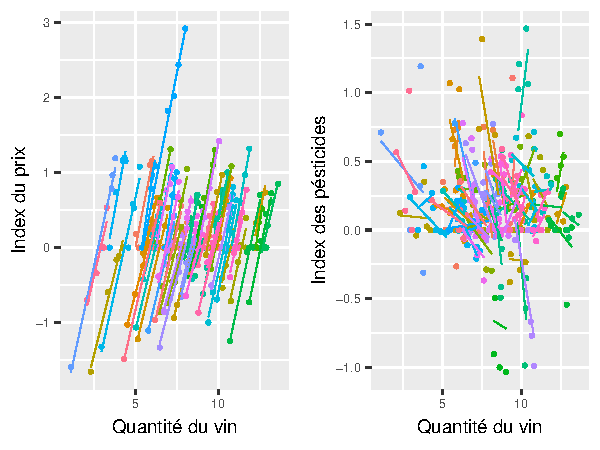
\includegraphics{Presentation_files/figure-beamer/unnamed-chunk-12-1.pdf}

\end{frame}

\begin{frame}[fragile]{Visualisatoin des interdependances}
\protect\hypertarget{visualisatoin-des-interdependances-1}{}

\begin{verbatim}
## `geom_smooth()` using method = 'loess' and formula 'y ~ x'
\end{verbatim}

\begin{verbatim}
## Warning in simpleLoess(y, x, w, span, degree = degree, parametric =
## parametric, : span too small. fewer data values than degrees of freedom.
\end{verbatim}

\begin{verbatim}
## Warning in simpleLoess(y, x, w, span, degree = degree, parametric =
## parametric, : pseudoinverse used at 9.2573
\end{verbatim}

\begin{verbatim}
## Warning in simpleLoess(y, x, w, span, degree = degree, parametric =
## parametric, : neighborhood radius 0.18005
\end{verbatim}

\begin{verbatim}
## Warning in simpleLoess(y, x, w, span, degree = degree, parametric =
## parametric, : reciprocal condition number 0
\end{verbatim}

\begin{verbatim}
## Warning in simpleLoess(y, x, w, span, degree = degree, parametric =
## parametric, : There are other near singularities as well. 0.014865
\end{verbatim}

\begin{verbatim}
## Warning in simpleLoess(y, x, w, span, degree = degree, parametric =
## parametric, : span too small. fewer data values than degrees of freedom.
\end{verbatim}

\begin{verbatim}
## Warning in simpleLoess(y, x, w, span, degree = degree, parametric =
## parametric, : pseudoinverse used at 5.0053
\end{verbatim}

\begin{verbatim}
## Warning in simpleLoess(y, x, w, span, degree = degree, parametric =
## parametric, : neighborhood radius 0.87248
\end{verbatim}

\begin{verbatim}
## Warning in simpleLoess(y, x, w, span, degree = degree, parametric =
## parametric, : reciprocal condition number 0
\end{verbatim}

\begin{verbatim}
## Warning in simpleLoess(y, x, w, span, degree = degree, parametric =
## parametric, : There are other near singularities as well. 0.045976
\end{verbatim}

\begin{verbatim}
## Warning in simpleLoess(y, x, w, span, degree = degree, parametric =
## parametric, : Chernobyl! trL>n 5

## Warning in simpleLoess(y, x, w, span, degree = degree, parametric =
## parametric, : Chernobyl! trL>n 5
\end{verbatim}

\begin{verbatim}
## Warning in sqrt(sum.squares/one.delta): production de NaN
\end{verbatim}

\begin{verbatim}
## Warning in simpleLoess(y, x, w, span, degree = degree, parametric =
## parametric, : span too small. fewer data values than degrees of freedom.
\end{verbatim}

\begin{verbatim}
## Warning in simpleLoess(y, x, w, span, degree = degree, parametric =
## parametric, : pseudoinverse used at 7.6162
\end{verbatim}

\begin{verbatim}
## Warning in simpleLoess(y, x, w, span, degree = degree, parametric =
## parametric, : neighborhood radius 0.3144
\end{verbatim}

\begin{verbatim}
## Warning in simpleLoess(y, x, w, span, degree = degree, parametric =
## parametric, : reciprocal condition number 0
\end{verbatim}

\begin{verbatim}
## Warning in simpleLoess(y, x, w, span, degree = degree, parametric =
## parametric, : There are other near singularities as well. 0.042878
\end{verbatim}

\begin{verbatim}
## Warning in simpleLoess(y, x, w, span, degree = degree, parametric =
## parametric, : Chernobyl! trL>n 5

## Warning in simpleLoess(y, x, w, span, degree = degree, parametric =
## parametric, : Chernobyl! trL>n 5
\end{verbatim}

\begin{verbatim}
## Warning in sqrt(sum.squares/one.delta): production de NaN
\end{verbatim}

\begin{verbatim}
## Warning in simpleLoess(y, x, w, span, degree = degree, parametric =
## parametric, : span too small. fewer data values than degrees of freedom.
\end{verbatim}

\begin{verbatim}
## Warning in simpleLoess(y, x, w, span, degree = degree, parametric =
## parametric, : pseudoinverse used at 8.2028
\end{verbatim}

\begin{verbatim}
## Warning in simpleLoess(y, x, w, span, degree = degree, parametric =
## parametric, : neighborhood radius 0.27479
\end{verbatim}

\begin{verbatim}
## Warning in simpleLoess(y, x, w, span, degree = degree, parametric =
## parametric, : reciprocal condition number 0
\end{verbatim}

\begin{verbatim}
## Warning in simpleLoess(y, x, w, span, degree = degree, parametric =
## parametric, : There are other near singularities as well. 0.18404
\end{verbatim}

\begin{verbatim}
## Warning in simpleLoess(y, x, w, span, degree = degree, parametric =
## parametric, : span too small. fewer data values than degrees of freedom.
\end{verbatim}

\begin{verbatim}
## Warning in simpleLoess(y, x, w, span, degree = degree, parametric =
## parametric, : pseudoinverse used at 5.7703
\end{verbatim}

\begin{verbatim}
## Warning in simpleLoess(y, x, w, span, degree = degree, parametric =
## parametric, : neighborhood radius 0.067414
\end{verbatim}

\begin{verbatim}
## Warning in simpleLoess(y, x, w, span, degree = degree, parametric =
## parametric, : reciprocal condition number 0
\end{verbatim}

\begin{verbatim}
## Warning in simpleLoess(y, x, w, span, degree = degree, parametric =
## parametric, : There are other near singularities as well. 0.025551
\end{verbatim}

\begin{verbatim}
## Warning in simpleLoess(y, x, w, span, degree = degree, parametric =
## parametric, : Chernobyl! trL>n 5

## Warning in simpleLoess(y, x, w, span, degree = degree, parametric =
## parametric, : Chernobyl! trL>n 5
\end{verbatim}

\begin{verbatim}
## Warning in sqrt(sum.squares/one.delta): production de NaN
\end{verbatim}

\begin{verbatim}
## Warning in simpleLoess(y, x, w, span, degree = degree, parametric =
## parametric, : span too small. fewer data values than degrees of freedom.
\end{verbatim}

\begin{verbatim}
## Warning in simpleLoess(y, x, w, span, degree = degree, parametric =
## parametric, : pseudoinverse used at 4.5043
\end{verbatim}

\begin{verbatim}
## Warning in simpleLoess(y, x, w, span, degree = degree, parametric =
## parametric, : neighborhood radius 0.96381
\end{verbatim}

\begin{verbatim}
## Warning in simpleLoess(y, x, w, span, degree = degree, parametric =
## parametric, : reciprocal condition number 0
\end{verbatim}

\begin{verbatim}
## Warning in simpleLoess(y, x, w, span, degree = degree, parametric =
## parametric, : There are other near singularities as well. 0.1394
\end{verbatim}

\begin{verbatim}
## Warning in simpleLoess(y, x, w, span, degree = degree, parametric =
## parametric, : Chernobyl! trL>n 5

## Warning in simpleLoess(y, x, w, span, degree = degree, parametric =
## parametric, : Chernobyl! trL>n 5
\end{verbatim}

\begin{verbatim}
## Warning in sqrt(sum.squares/one.delta): production de NaN
\end{verbatim}

\begin{verbatim}
## Warning in simpleLoess(y, x, w, span, degree = degree, parametric =
## parametric, : span too small. fewer data values than degrees of freedom.
\end{verbatim}

\begin{verbatim}
## Warning in simpleLoess(y, x, w, span, degree = degree, parametric =
## parametric, : pseudoinverse used at 9.9129
\end{verbatim}

\begin{verbatim}
## Warning in simpleLoess(y, x, w, span, degree = degree, parametric =
## parametric, : neighborhood radius 0.20921
\end{verbatim}

\begin{verbatim}
## Warning in simpleLoess(y, x, w, span, degree = degree, parametric =
## parametric, : reciprocal condition number 0
\end{verbatim}

\begin{verbatim}
## Warning in simpleLoess(y, x, w, span, degree = degree, parametric =
## parametric, : There are other near singularities as well. 0.38525
\end{verbatim}

\begin{verbatim}
## Warning in simpleLoess(y, x, w, span, degree = degree, parametric =
## parametric, : span too small. fewer data values than degrees of freedom.
\end{verbatim}

\begin{verbatim}
## Warning in simpleLoess(y, x, w, span, degree = degree, parametric =
## parametric, : pseudoinverse used at 5.4467
\end{verbatim}

\begin{verbatim}
## Warning in simpleLoess(y, x, w, span, degree = degree, parametric =
## parametric, : neighborhood radius 0.33712
\end{verbatim}

\begin{verbatim}
## Warning in simpleLoess(y, x, w, span, degree = degree, parametric =
## parametric, : reciprocal condition number 0
\end{verbatim}

\begin{verbatim}
## Warning in simpleLoess(y, x, w, span, degree = degree, parametric =
## parametric, : There are other near singularities as well. 0.28909
\end{verbatim}

\begin{verbatim}
## Warning in simpleLoess(y, x, w, span, degree = degree, parametric =
## parametric, : span too small. fewer data values than degrees of freedom.
\end{verbatim}

\begin{verbatim}
## Warning in simpleLoess(y, x, w, span, degree = degree, parametric =
## parametric, : pseudoinverse used at 5.1268
\end{verbatim}

\begin{verbatim}
## Warning in simpleLoess(y, x, w, span, degree = degree, parametric =
## parametric, : neighborhood radius 1.5299
\end{verbatim}

\begin{verbatim}
## Warning in simpleLoess(y, x, w, span, degree = degree, parametric =
## parametric, : reciprocal condition number 0
\end{verbatim}

\begin{verbatim}
## Warning in simpleLoess(y, x, w, span, degree = degree, parametric =
## parametric, : There are other near singularities as well. 0.078834
\end{verbatim}

\begin{verbatim}
## Warning in simpleLoess(y, x, w, span, degree = degree, parametric =
## parametric, : span too small. fewer data values than degrees of freedom.
\end{verbatim}

\begin{verbatim}
## Warning in simpleLoess(y, x, w, span, degree = degree, parametric =
## parametric, : pseudoinverse used at 12.237
\end{verbatim}

\begin{verbatim}
## Warning in simpleLoess(y, x, w, span, degree = degree, parametric =
## parametric, : neighborhood radius 0.29044
\end{verbatim}

\begin{verbatim}
## Warning in simpleLoess(y, x, w, span, degree = degree, parametric =
## parametric, : reciprocal condition number 0
\end{verbatim}

\begin{verbatim}
## Warning in simpleLoess(y, x, w, span, degree = degree, parametric =
## parametric, : There are other near singularities as well. 0.096775
\end{verbatim}

\begin{verbatim}
## Warning in simpleLoess(y, x, w, span, degree = degree, parametric =
## parametric, : span too small. fewer data values than degrees of freedom.
\end{verbatim}

\begin{verbatim}
## Warning in simpleLoess(y, x, w, span, degree = degree, parametric =
## parametric, : pseudoinverse used at 7.3144
\end{verbatim}

\begin{verbatim}
## Warning in simpleLoess(y, x, w, span, degree = degree, parametric =
## parametric, : neighborhood radius 0.95279
\end{verbatim}

\begin{verbatim}
## Warning in simpleLoess(y, x, w, span, degree = degree, parametric =
## parametric, : reciprocal condition number 0
\end{verbatim}

\begin{verbatim}
## Warning in simpleLoess(y, x, w, span, degree = degree, parametric =
## parametric, : There are other near singularities as well. 0.080618
\end{verbatim}

\begin{verbatim}
## Warning in simpleLoess(y, x, w, span, degree = degree, parametric =
## parametric, : Chernobyl! trL>n 5

## Warning in simpleLoess(y, x, w, span, degree = degree, parametric =
## parametric, : Chernobyl! trL>n 5
\end{verbatim}

\begin{verbatim}
## Warning in sqrt(sum.squares/one.delta): production de NaN
\end{verbatim}

\begin{verbatim}
## Warning in simpleLoess(y, x, w, span, degree = degree, parametric =
## parametric, : span too small. fewer data values than degrees of freedom.
\end{verbatim}

\begin{verbatim}
## Warning in simpleLoess(y, x, w, span, degree = degree, parametric =
## parametric, : pseudoinverse used at 9.2547
\end{verbatim}

\begin{verbatim}
## Warning in simpleLoess(y, x, w, span, degree = degree, parametric =
## parametric, : neighborhood radius 0.27472
\end{verbatim}

\begin{verbatim}
## Warning in simpleLoess(y, x, w, span, degree = degree, parametric =
## parametric, : reciprocal condition number 0
\end{verbatim}

\begin{verbatim}
## Warning in simpleLoess(y, x, w, span, degree = degree, parametric =
## parametric, : There are other near singularities as well. 0.53273
\end{verbatim}

\begin{verbatim}
## Warning in simpleLoess(y, x, w, span, degree = degree, parametric =
## parametric, : span too small. fewer data values than degrees of freedom.
\end{verbatim}

\begin{verbatim}
## Warning in simpleLoess(y, x, w, span, degree = degree, parametric =
## parametric, : pseudoinverse used at 2.293
\end{verbatim}

\begin{verbatim}
## Warning in simpleLoess(y, x, w, span, degree = degree, parametric =
## parametric, : neighborhood radius 1.5571
\end{verbatim}

\begin{verbatim}
## Warning in simpleLoess(y, x, w, span, degree = degree, parametric =
## parametric, : reciprocal condition number 0
\end{verbatim}

\begin{verbatim}
## Warning in simpleLoess(y, x, w, span, degree = degree, parametric =
## parametric, : There are other near singularities as well. 0.15493
\end{verbatim}

\begin{verbatim}
## Warning in simpleLoess(y, x, w, span, degree = degree, parametric =
## parametric, : Chernobyl! trL>n 5

## Warning in simpleLoess(y, x, w, span, degree = degree, parametric =
## parametric, : Chernobyl! trL>n 5
\end{verbatim}

\begin{verbatim}
## Warning in sqrt(sum.squares/one.delta): production de NaN
\end{verbatim}

\begin{verbatim}
## Warning in simpleLoess(y, x, w, span, degree = degree, parametric =
## parametric, : span too small. fewer data values than degrees of freedom.
\end{verbatim}

\begin{verbatim}
## Warning in simpleLoess(y, x, w, span, degree = degree, parametric =
## parametric, : pseudoinverse used at 10.225
\end{verbatim}

\begin{verbatim}
## Warning in simpleLoess(y, x, w, span, degree = degree, parametric =
## parametric, : neighborhood radius 0.22617
\end{verbatim}

\begin{verbatim}
## Warning in simpleLoess(y, x, w, span, degree = degree, parametric =
## parametric, : reciprocal condition number 0
\end{verbatim}

\begin{verbatim}
## Warning in simpleLoess(y, x, w, span, degree = degree, parametric =
## parametric, : There are other near singularities as well. 0.23941
\end{verbatim}

\begin{verbatim}
## Warning in simpleLoess(y, x, w, span, degree = degree, parametric =
## parametric, : span too small. fewer data values than degrees of freedom.
\end{verbatim}

\begin{verbatim}
## Warning in simpleLoess(y, x, w, span, degree = degree, parametric =
## parametric, : pseudoinverse used at 10.753
\end{verbatim}

\begin{verbatim}
## Warning in simpleLoess(y, x, w, span, degree = degree, parametric =
## parametric, : neighborhood radius 0.60825
\end{verbatim}

\begin{verbatim}
## Warning in simpleLoess(y, x, w, span, degree = degree, parametric =
## parametric, : reciprocal condition number 0
\end{verbatim}

\begin{verbatim}
## Warning in simpleLoess(y, x, w, span, degree = degree, parametric =
## parametric, : There are other near singularities as well. 0.099223
\end{verbatim}

\begin{verbatim}
## Warning in simpleLoess(y, x, w, span, degree = degree, parametric =
## parametric, : span too small. fewer data values than degrees of freedom.
\end{verbatim}

\begin{verbatim}
## Warning in simpleLoess(y, x, w, span, degree = degree, parametric =
## parametric, : pseudoinverse used at 6.4843
\end{verbatim}

\begin{verbatim}
## Warning in simpleLoess(y, x, w, span, degree = degree, parametric =
## parametric, : neighborhood radius 1.1495
\end{verbatim}

\begin{verbatim}
## Warning in simpleLoess(y, x, w, span, degree = degree, parametric =
## parametric, : reciprocal condition number 0
\end{verbatim}

\begin{verbatim}
## Warning in simpleLoess(y, x, w, span, degree = degree, parametric =
## parametric, : There are other near singularities as well. 0.019423
\end{verbatim}

\begin{verbatim}
## Warning in simpleLoess(y, x, w, span, degree = degree, parametric =
## parametric, : span too small. fewer data values than degrees of freedom.
\end{verbatim}

\begin{verbatim}
## Warning in simpleLoess(y, x, w, span, degree = degree, parametric =
## parametric, : pseudoinverse used at 6.9468
\end{verbatim}

\begin{verbatim}
## Warning in simpleLoess(y, x, w, span, degree = degree, parametric =
## parametric, : neighborhood radius 0.41839
\end{verbatim}

\begin{verbatim}
## Warning in simpleLoess(y, x, w, span, degree = degree, parametric =
## parametric, : reciprocal condition number 0
\end{verbatim}

\begin{verbatim}
## Warning in simpleLoess(y, x, w, span, degree = degree, parametric =
## parametric, : There are other near singularities as well. 0.34638
\end{verbatim}

\begin{verbatim}
## Warning in simpleLoess(y, x, w, span, degree = degree, parametric =
## parametric, : span too small. fewer data values than degrees of freedom.
\end{verbatim}

\begin{verbatim}
## Warning in simpleLoess(y, x, w, span, degree = degree, parametric =
## parametric, : pseudoinverse used at 6.5674
\end{verbatim}

\begin{verbatim}
## Warning in simpleLoess(y, x, w, span, degree = degree, parametric =
## parametric, : neighborhood radius 0.83082
\end{verbatim}

\begin{verbatim}
## Warning in simpleLoess(y, x, w, span, degree = degree, parametric =
## parametric, : reciprocal condition number 0
\end{verbatim}

\begin{verbatim}
## Warning in simpleLoess(y, x, w, span, degree = degree, parametric =
## parametric, : There are other near singularities as well. 0.53223
\end{verbatim}

\begin{verbatim}
## Warning in simpleLoess(y, x, w, span, degree = degree, parametric =
## parametric, : span too small. fewer data values than degrees of freedom.
\end{verbatim}

\begin{verbatim}
## Warning in simpleLoess(y, x, w, span, degree = degree, parametric =
## parametric, : pseudoinverse used at 9.5597
\end{verbatim}

\begin{verbatim}
## Warning in simpleLoess(y, x, w, span, degree = degree, parametric =
## parametric, : neighborhood radius 0.41892
\end{verbatim}

\begin{verbatim}
## Warning in simpleLoess(y, x, w, span, degree = degree, parametric =
## parametric, : reciprocal condition number 0
\end{verbatim}

\begin{verbatim}
## Warning in simpleLoess(y, x, w, span, degree = degree, parametric =
## parametric, : There are other near singularities as well. 0.68519
\end{verbatim}

\begin{verbatim}
## Warning in simpleLoess(y, x, w, span, degree = degree, parametric =
## parametric, : span too small. fewer data values than degrees of freedom.
\end{verbatim}

\begin{verbatim}
## Warning in simpleLoess(y, x, w, span, degree = degree, parametric =
## parametric, : pseudoinverse used at 5.9933
\end{verbatim}

\begin{verbatim}
## Warning in simpleLoess(y, x, w, span, degree = degree, parametric =
## parametric, : neighborhood radius 0.12696
\end{verbatim}

\begin{verbatim}
## Warning in simpleLoess(y, x, w, span, degree = degree, parametric =
## parametric, : reciprocal condition number 0
\end{verbatim}

\begin{verbatim}
## Warning in simpleLoess(y, x, w, span, degree = degree, parametric =
## parametric, : There are other near singularities as well. 1.0066
\end{verbatim}

\begin{verbatim}
## Warning in simpleLoess(y, x, w, span, degree = degree, parametric =
## parametric, : span too small. fewer data values than degrees of freedom.
\end{verbatim}

\begin{verbatim}
## Warning in simpleLoess(y, x, w, span, degree = degree, parametric =
## parametric, : pseudoinverse used at 8.5536
\end{verbatim}

\begin{verbatim}
## Warning in simpleLoess(y, x, w, span, degree = degree, parametric =
## parametric, : neighborhood radius 0.60138
\end{verbatim}

\begin{verbatim}
## Warning in simpleLoess(y, x, w, span, degree = degree, parametric =
## parametric, : reciprocal condition number 0
\end{verbatim}

\begin{verbatim}
## Warning in simpleLoess(y, x, w, span, degree = degree, parametric =
## parametric, : There are other near singularities as well. 0.45536
\end{verbatim}

\begin{verbatim}
## Warning in simpleLoess(y, x, w, span, degree = degree, parametric =
## parametric, : span too small. fewer data values than degrees of freedom.
\end{verbatim}

\begin{verbatim}
## Warning in simpleLoess(y, x, w, span, degree = degree, parametric =
## parametric, : pseudoinverse used at 12.252
\end{verbatim}

\begin{verbatim}
## Warning in simpleLoess(y, x, w, span, degree = degree, parametric =
## parametric, : neighborhood radius 0.19328
\end{verbatim}

\begin{verbatim}
## Warning in simpleLoess(y, x, w, span, degree = degree, parametric =
## parametric, : reciprocal condition number 0
\end{verbatim}

\begin{verbatim}
## Warning in simpleLoess(y, x, w, span, degree = degree, parametric =
## parametric, : There are other near singularities as well. 0.050849
\end{verbatim}

\begin{verbatim}
## Warning in simpleLoess(y, x, w, span, degree = degree, parametric =
## parametric, : span too small. fewer data values than degrees of freedom.
\end{verbatim}

\begin{verbatim}
## Warning in simpleLoess(y, x, w, span, degree = degree, parametric =
## parametric, : pseudoinverse used at 8.247
\end{verbatim}

\begin{verbatim}
## Warning in simpleLoess(y, x, w, span, degree = degree, parametric =
## parametric, : neighborhood radius 0.36587
\end{verbatim}

\begin{verbatim}
## Warning in simpleLoess(y, x, w, span, degree = degree, parametric =
## parametric, : reciprocal condition number 0
\end{verbatim}

\begin{verbatim}
## Warning in simpleLoess(y, x, w, span, degree = degree, parametric =
## parametric, : There are other near singularities as well. 0.17566
\end{verbatim}

\begin{verbatim}
## Warning in simpleLoess(y, x, w, span, degree = degree, parametric =
## parametric, : span too small. fewer data values than degrees of freedom.
\end{verbatim}

\begin{verbatim}
## Warning in simpleLoess(y, x, w, span, degree = degree, parametric =
## parametric, : pseudoinverse used at 11.86
\end{verbatim}

\begin{verbatim}
## Warning in simpleLoess(y, x, w, span, degree = degree, parametric =
## parametric, : neighborhood radius 0.9666
\end{verbatim}

\begin{verbatim}
## Warning in simpleLoess(y, x, w, span, degree = degree, parametric =
## parametric, : reciprocal condition number 0
\end{verbatim}

\begin{verbatim}
## Warning in simpleLoess(y, x, w, span, degree = degree, parametric =
## parametric, : There are other near singularities as well. 0.13913
\end{verbatim}

\begin{verbatim}
## Warning in simpleLoess(y, x, w, span, degree = degree, parametric =
## parametric, : span too small. fewer data values than degrees of freedom.
\end{verbatim}

\begin{verbatim}
## Warning in simpleLoess(y, x, w, span, degree = degree, parametric =
## parametric, : pseudoinverse used at 10.706
\end{verbatim}

\begin{verbatim}
## Warning in simpleLoess(y, x, w, span, degree = degree, parametric =
## parametric, : neighborhood radius 1.1776
\end{verbatim}

\begin{verbatim}
## Warning in simpleLoess(y, x, w, span, degree = degree, parametric =
## parametric, : reciprocal condition number 0
\end{verbatim}

\begin{verbatim}
## Warning in simpleLoess(y, x, w, span, degree = degree, parametric =
## parametric, : There are other near singularities as well. 0.44166
\end{verbatim}

\begin{verbatim}
## Warning in simpleLoess(y, x, w, span, degree = degree, parametric =
## parametric, : span too small. fewer data values than degrees of freedom.
\end{verbatim}

\begin{verbatim}
## Warning in simpleLoess(y, x, w, span, degree = degree, parametric =
## parametric, : pseudoinverse used at 12.633
\end{verbatim}

\begin{verbatim}
## Warning in simpleLoess(y, x, w, span, degree = degree, parametric =
## parametric, : neighborhood radius 0.35048
\end{verbatim}

\begin{verbatim}
## Warning in simpleLoess(y, x, w, span, degree = degree, parametric =
## parametric, : reciprocal condition number 0
\end{verbatim}

\begin{verbatim}
## Warning in simpleLoess(y, x, w, span, degree = degree, parametric =
## parametric, : There are other near singularities as well. 0.42041
\end{verbatim}

\begin{verbatim}
## Warning in simpleLoess(y, x, w, span, degree = degree, parametric =
## parametric, : Chernobyl! trL>n 5

## Warning in simpleLoess(y, x, w, span, degree = degree, parametric =
## parametric, : Chernobyl! trL>n 5
\end{verbatim}

\begin{verbatim}
## Warning in sqrt(sum.squares/one.delta): production de NaN
\end{verbatim}

\begin{verbatim}
## Warning in simpleLoess(y, x, w, span, degree = degree, parametric =
## parametric, : span too small. fewer data values than degrees of freedom.
\end{verbatim}

\begin{verbatim}
## Warning in simpleLoess(y, x, w, span, degree = degree, parametric =
## parametric, : pseudoinverse used at 7.9104
\end{verbatim}

\begin{verbatim}
## Warning in simpleLoess(y, x, w, span, degree = degree, parametric =
## parametric, : neighborhood radius 0.46314
\end{verbatim}

\begin{verbatim}
## Warning in simpleLoess(y, x, w, span, degree = degree, parametric =
## parametric, : reciprocal condition number 0
\end{verbatim}

\begin{verbatim}
## Warning in simpleLoess(y, x, w, span, degree = degree, parametric =
## parametric, : There are other near singularities as well. 0.1493
\end{verbatim}

\begin{verbatim}
## Warning in simpleLoess(y, x, w, span, degree = degree, parametric =
## parametric, : Chernobyl! trL>n 5

## Warning in simpleLoess(y, x, w, span, degree = degree, parametric =
## parametric, : Chernobyl! trL>n 5
\end{verbatim}

\begin{verbatim}
## Warning in sqrt(sum.squares/one.delta): production de NaN
\end{verbatim}

\begin{verbatim}
## Warning in simpleLoess(y, x, w, span, degree = degree, parametric =
## parametric, : span too small. fewer data values than degrees of freedom.
\end{verbatim}

\begin{verbatim}
## Warning in simpleLoess(y, x, w, span, degree = degree, parametric =
## parametric, : pseudoinverse used at 9.7808
\end{verbatim}

\begin{verbatim}
## Warning in simpleLoess(y, x, w, span, degree = degree, parametric =
## parametric, : neighborhood radius 0.44022
\end{verbatim}

\begin{verbatim}
## Warning in simpleLoess(y, x, w, span, degree = degree, parametric =
## parametric, : reciprocal condition number 0
\end{verbatim}

\begin{verbatim}
## Warning in simpleLoess(y, x, w, span, degree = degree, parametric =
## parametric, : There are other near singularities as well. 0.0060322
\end{verbatim}

\begin{verbatim}
## Warning in simpleLoess(y, x, w, span, degree = degree, parametric =
## parametric, : span too small. fewer data values than degrees of freedom.
\end{verbatim}

\begin{verbatim}
## Warning in simpleLoess(y, x, w, span, degree = degree, parametric =
## parametric, : pseudoinverse used at 8.5771
\end{verbatim}

\begin{verbatim}
## Warning in simpleLoess(y, x, w, span, degree = degree, parametric =
## parametric, : neighborhood radius 0.25238
\end{verbatim}

\begin{verbatim}
## Warning in simpleLoess(y, x, w, span, degree = degree, parametric =
## parametric, : reciprocal condition number 0
\end{verbatim}

\begin{verbatim}
## Warning in simpleLoess(y, x, w, span, degree = degree, parametric =
## parametric, : There are other near singularities as well. 0.080334
\end{verbatim}

\begin{verbatim}
## Warning in simpleLoess(y, x, w, span, degree = degree, parametric =
## parametric, : span too small. fewer data values than degrees of freedom.
\end{verbatim}

\begin{verbatim}
## Warning in simpleLoess(y, x, w, span, degree = degree, parametric =
## parametric, : pseudoinverse used at 8.1538
\end{verbatim}

\begin{verbatim}
## Warning in simpleLoess(y, x, w, span, degree = degree, parametric =
## parametric, : neighborhood radius 0.23551
\end{verbatim}

\begin{verbatim}
## Warning in simpleLoess(y, x, w, span, degree = degree, parametric =
## parametric, : reciprocal condition number 0
\end{verbatim}

\begin{verbatim}
## Warning in simpleLoess(y, x, w, span, degree = degree, parametric =
## parametric, : There are other near singularities as well. 0.12959
\end{verbatim}

\begin{verbatim}
## Warning in simpleLoess(y, x, w, span, degree = degree, parametric =
## parametric, : span too small. fewer data values than degrees of freedom.
\end{verbatim}

\begin{verbatim}
## Warning in simpleLoess(y, x, w, span, degree = degree, parametric =
## parametric, : pseudoinverse used at 9.0761
\end{verbatim}

\begin{verbatim}
## Warning in simpleLoess(y, x, w, span, degree = degree, parametric =
## parametric, : neighborhood radius 0.83298
\end{verbatim}

\begin{verbatim}
## Warning in simpleLoess(y, x, w, span, degree = degree, parametric =
## parametric, : reciprocal condition number 0
\end{verbatim}

\begin{verbatim}
## Warning in simpleLoess(y, x, w, span, degree = degree, parametric =
## parametric, : There are other near singularities as well. 0.43365
\end{verbatim}

\begin{verbatim}
## Warning in simpleLoess(y, x, w, span, degree = degree, parametric =
## parametric, : Chernobyl! trL>n 5

## Warning in simpleLoess(y, x, w, span, degree = degree, parametric =
## parametric, : Chernobyl! trL>n 5
\end{verbatim}

\begin{verbatim}
## Warning in sqrt(sum.squares/one.delta): production de NaN
\end{verbatim}

\begin{verbatim}
## Warning in simpleLoess(y, x, w, span, degree = degree, parametric =
## parametric, : span too small. fewer data values than degrees of freedom.
\end{verbatim}

\begin{verbatim}
## Warning in simpleLoess(y, x, w, span, degree = degree, parametric =
## parametric, : pseudoinverse used at 9.8022
\end{verbatim}

\begin{verbatim}
## Warning in simpleLoess(y, x, w, span, degree = degree, parametric =
## parametric, : neighborhood radius 0.059584
\end{verbatim}

\begin{verbatim}
## Warning in simpleLoess(y, x, w, span, degree = degree, parametric =
## parametric, : reciprocal condition number 0
\end{verbatim}

\begin{verbatim}
## Warning in simpleLoess(y, x, w, span, degree = degree, parametric =
## parametric, : There are other near singularities as well. 0.31545
\end{verbatim}

\begin{verbatim}
## Warning in simpleLoess(y, x, w, span, degree = degree, parametric =
## parametric, : span too small. fewer data values than degrees of freedom.
\end{verbatim}

\begin{verbatim}
## Warning in simpleLoess(y, x, w, span, degree = degree, parametric =
## parametric, : pseudoinverse used at 8.3937
\end{verbatim}

\begin{verbatim}
## Warning in simpleLoess(y, x, w, span, degree = degree, parametric =
## parametric, : neighborhood radius 0.39964
\end{verbatim}

\begin{verbatim}
## Warning in simpleLoess(y, x, w, span, degree = degree, parametric =
## parametric, : reciprocal condition number 0
\end{verbatim}

\begin{verbatim}
## Warning in simpleLoess(y, x, w, span, degree = degree, parametric =
## parametric, : There are other near singularities as well. 0.037518
\end{verbatim}

\begin{verbatim}
## Warning in simpleLoess(y, x, w, span, degree = degree, parametric =
## parametric, : Chernobyl! trL>n 5

## Warning in simpleLoess(y, x, w, span, degree = degree, parametric =
## parametric, : Chernobyl! trL>n 5
\end{verbatim}

\begin{verbatim}
## Warning in sqrt(sum.squares/one.delta): production de NaN
\end{verbatim}

\begin{verbatim}
## Warning in simpleLoess(y, x, w, span, degree = degree, parametric =
## parametric, : span too small. fewer data values than degrees of freedom.
\end{verbatim}

\begin{verbatim}
## Warning in simpleLoess(y, x, w, span, degree = degree, parametric =
## parametric, : pseudoinverse used at 5.0238
\end{verbatim}

\begin{verbatim}
## Warning in simpleLoess(y, x, w, span, degree = degree, parametric =
## parametric, : neighborhood radius 1.2898
\end{verbatim}

\begin{verbatim}
## Warning in simpleLoess(y, x, w, span, degree = degree, parametric =
## parametric, : reciprocal condition number 0
\end{verbatim}

\begin{verbatim}
## Warning in simpleLoess(y, x, w, span, degree = degree, parametric =
## parametric, : There are other near singularities as well. 0.0033494
\end{verbatim}

\begin{verbatim}
## Warning in simpleLoess(y, x, w, span, degree = degree, parametric =
## parametric, : span too small. fewer data values than degrees of freedom.
\end{verbatim}

\begin{verbatim}
## Warning in simpleLoess(y, x, w, span, degree = degree, parametric =
## parametric, : pseudoinverse used at 10.822
\end{verbatim}

\begin{verbatim}
## Warning in simpleLoess(y, x, w, span, degree = degree, parametric =
## parametric, : neighborhood radius 0.53267
\end{verbatim}

\begin{verbatim}
## Warning in simpleLoess(y, x, w, span, degree = degree, parametric =
## parametric, : reciprocal condition number 0
\end{verbatim}

\begin{verbatim}
## Warning in simpleLoess(y, x, w, span, degree = degree, parametric =
## parametric, : There are other near singularities as well. 0.28123
\end{verbatim}

\begin{verbatim}
## Warning in simpleLoess(y, x, w, span, degree = degree, parametric =
## parametric, : Chernobyl! trL>n 5

## Warning in simpleLoess(y, x, w, span, degree = degree, parametric =
## parametric, : Chernobyl! trL>n 5
\end{verbatim}

\begin{verbatim}
## Warning in sqrt(sum.squares/one.delta): production de NaN
\end{verbatim}

\begin{verbatim}
## Warning in simpleLoess(y, x, w, span, degree = degree, parametric =
## parametric, : span too small. fewer data values than degrees of freedom.
\end{verbatim}

\begin{verbatim}
## Warning in simpleLoess(y, x, w, span, degree = degree, parametric =
## parametric, : pseudoinverse used at 5.4583
\end{verbatim}

\begin{verbatim}
## Warning in simpleLoess(y, x, w, span, degree = degree, parametric =
## parametric, : neighborhood radius 0.69866
\end{verbatim}

\begin{verbatim}
## Warning in simpleLoess(y, x, w, span, degree = degree, parametric =
## parametric, : reciprocal condition number 0
\end{verbatim}

\begin{verbatim}
## Warning in simpleLoess(y, x, w, span, degree = degree, parametric =
## parametric, : There are other near singularities as well. 0.1724
\end{verbatim}

\begin{verbatim}
## Warning in simpleLoess(y, x, w, span, degree = degree, parametric =
## parametric, : span too small. fewer data values than degrees of freedom.
\end{verbatim}

\begin{verbatim}
## Warning in simpleLoess(y, x, w, span, degree = degree, parametric =
## parametric, : pseudoinverse used at 9.4008
\end{verbatim}

\begin{verbatim}
## Warning in simpleLoess(y, x, w, span, degree = degree, parametric =
## parametric, : neighborhood radius 0.84815
\end{verbatim}

\begin{verbatim}
## Warning in simpleLoess(y, x, w, span, degree = degree, parametric =
## parametric, : reciprocal condition number 0
\end{verbatim}

\begin{verbatim}
## Warning in simpleLoess(y, x, w, span, degree = degree, parametric =
## parametric, : There are other near singularities as well. 0.28886
\end{verbatim}

\begin{verbatim}
## Warning in simpleLoess(y, x, w, span, degree = degree, parametric =
## parametric, : span too small. fewer data values than degrees of freedom.
\end{verbatim}

\begin{verbatim}
## Warning in simpleLoess(y, x, w, span, degree = degree, parametric =
## parametric, : pseudoinverse used at 9.9168
\end{verbatim}

\begin{verbatim}
## Warning in simpleLoess(y, x, w, span, degree = degree, parametric =
## parametric, : neighborhood radius 0.75055
\end{verbatim}

\begin{verbatim}
## Warning in simpleLoess(y, x, w, span, degree = degree, parametric =
## parametric, : reciprocal condition number 0
\end{verbatim}

\begin{verbatim}
## Warning in simpleLoess(y, x, w, span, degree = degree, parametric =
## parametric, : There are other near singularities as well. 0.1819
\end{verbatim}

\begin{verbatim}
## Warning in simpleLoess(y, x, w, span, degree = degree, parametric =
## parametric, : span too small. fewer data values than degrees of freedom.
\end{verbatim}

\begin{verbatim}
## Warning in simpleLoess(y, x, w, span, degree = degree, parametric =
## parametric, : pseudoinverse used at 10.435
\end{verbatim}

\begin{verbatim}
## Warning in simpleLoess(y, x, w, span, degree = degree, parametric =
## parametric, : neighborhood radius 0.37465
\end{verbatim}

\begin{verbatim}
## Warning in simpleLoess(y, x, w, span, degree = degree, parametric =
## parametric, : reciprocal condition number 0
\end{verbatim}

\begin{verbatim}
## Warning in simpleLoess(y, x, w, span, degree = degree, parametric =
## parametric, : There are other near singularities as well. 0.0089543
\end{verbatim}

\begin{verbatim}
## Warning in simpleLoess(y, x, w, span, degree = degree, parametric =
## parametric, : span too small. fewer data values than degrees of freedom.
\end{verbatim}

\begin{verbatim}
## Warning in simpleLoess(y, x, w, span, degree = degree, parametric =
## parametric, : pseudoinverse used at 2.933
\end{verbatim}

\begin{verbatim}
## Warning in simpleLoess(y, x, w, span, degree = degree, parametric =
## parametric, : neighborhood radius 1.9191
\end{verbatim}

\begin{verbatim}
## Warning in simpleLoess(y, x, w, span, degree = degree, parametric =
## parametric, : reciprocal condition number 0
\end{verbatim}

\begin{verbatim}
## Warning in simpleLoess(y, x, w, span, degree = degree, parametric =
## parametric, : There are other near singularities as well. 0.16956
\end{verbatim}

\begin{verbatim}
## Warning in simpleLoess(y, x, w, span, degree = degree, parametric =
## parametric, : Chernobyl! trL>n 5

## Warning in simpleLoess(y, x, w, span, degree = degree, parametric =
## parametric, : Chernobyl! trL>n 5
\end{verbatim}

\begin{verbatim}
## Warning in sqrt(sum.squares/one.delta): production de NaN
\end{verbatim}

\begin{verbatim}
## Warning in simpleLoess(y, x, w, span, degree = degree, parametric =
## parametric, : span too small. fewer data values than degrees of freedom.
\end{verbatim}

\begin{verbatim}
## Warning in simpleLoess(y, x, w, span, degree = degree, parametric =
## parametric, : pseudoinverse used at 6.3397
\end{verbatim}

\begin{verbatim}
## Warning in simpleLoess(y, x, w, span, degree = degree, parametric =
## parametric, : neighborhood radius 0.24095
\end{verbatim}

\begin{verbatim}
## Warning in simpleLoess(y, x, w, span, degree = degree, parametric =
## parametric, : reciprocal condition number 0
\end{verbatim}

\begin{verbatim}
## Warning in simpleLoess(y, x, w, span, degree = degree, parametric =
## parametric, : There are other near singularities as well. 0.3662
\end{verbatim}

\begin{verbatim}
## Warning in simpleLoess(y, x, w, span, degree = degree, parametric =
## parametric, : span too small. fewer data values than degrees of freedom.
\end{verbatim}

\begin{verbatim}
## Warning in simpleLoess(y, x, w, span, degree = degree, parametric =
## parametric, : pseudoinverse used at 3.4292
\end{verbatim}

\begin{verbatim}
## Warning in simpleLoess(y, x, w, span, degree = degree, parametric =
## parametric, : neighborhood radius 0.79031
\end{verbatim}

\begin{verbatim}
## Warning in simpleLoess(y, x, w, span, degree = degree, parametric =
## parametric, : reciprocal condition number 0
\end{verbatim}

\begin{verbatim}
## Warning in simpleLoess(y, x, w, span, degree = degree, parametric =
## parametric, : There are other near singularities as well. 0.032307
\end{verbatim}

\begin{verbatim}
## Warning in simpleLoess(y, x, w, span, degree = degree, parametric =
## parametric, : span too small. fewer data values than degrees of freedom.
\end{verbatim}

\begin{verbatim}
## Warning in simpleLoess(y, x, w, span, degree = degree, parametric =
## parametric, : pseudoinverse used at 6.7945
\end{verbatim}

\begin{verbatim}
## Warning in simpleLoess(y, x, w, span, degree = degree, parametric =
## parametric, : neighborhood radius 0.52667
\end{verbatim}

\begin{verbatim}
## Warning in simpleLoess(y, x, w, span, degree = degree, parametric =
## parametric, : reciprocal condition number 0
\end{verbatim}

\begin{verbatim}
## Warning in simpleLoess(y, x, w, span, degree = degree, parametric =
## parametric, : There are other near singularities as well. 0.027384
\end{verbatim}

\begin{verbatim}
## Warning in simpleLoess(y, x, w, span, degree = degree, parametric =
## parametric, : Chernobyl! trL>n 5

## Warning in simpleLoess(y, x, w, span, degree = degree, parametric =
## parametric, : Chernobyl! trL>n 5
\end{verbatim}

\begin{verbatim}
## Warning in sqrt(sum.squares/one.delta): production de NaN
\end{verbatim}

\begin{verbatim}
## Warning in simpleLoess(y, x, w, span, degree = degree, parametric =
## parametric, : span too small. fewer data values than degrees of freedom.
\end{verbatim}

\begin{verbatim}
## Warning in simpleLoess(y, x, w, span, degree = degree, parametric =
## parametric, : pseudoinverse used at 5.3898
\end{verbatim}

\begin{verbatim}
## Warning in simpleLoess(y, x, w, span, degree = degree, parametric =
## parametric, : neighborhood radius 0.56865
\end{verbatim}

\begin{verbatim}
## Warning in simpleLoess(y, x, w, span, degree = degree, parametric =
## parametric, : reciprocal condition number 0
\end{verbatim}

\begin{verbatim}
## Warning in simpleLoess(y, x, w, span, degree = degree, parametric =
## parametric, : There are other near singularities as well. 0.044458
\end{verbatim}

\begin{verbatim}
## Warning in simpleLoess(y, x, w, span, degree = degree, parametric =
## parametric, : span too small. fewer data values than degrees of freedom.
\end{verbatim}

\begin{verbatim}
## Warning in simpleLoess(y, x, w, span, degree = degree, parametric =
## parametric, : pseudoinverse used at 5.4638
\end{verbatim}

\begin{verbatim}
## Warning in simpleLoess(y, x, w, span, degree = degree, parametric =
## parametric, : neighborhood radius 1.8613
\end{verbatim}

\begin{verbatim}
## Warning in simpleLoess(y, x, w, span, degree = degree, parametric =
## parametric, : reciprocal condition number 0
\end{verbatim}

\begin{verbatim}
## Warning in simpleLoess(y, x, w, span, degree = degree, parametric =
## parametric, : There are other near singularities as well. 0.48424
\end{verbatim}

\begin{verbatim}
## Warning in simpleLoess(y, x, w, span, degree = degree, parametric =
## parametric, : span too small. fewer data values than degrees of freedom.
\end{verbatim}

\begin{verbatim}
## Warning in simpleLoess(y, x, w, span, degree = degree, parametric =
## parametric, : pseudoinverse used at 5.7667
\end{verbatim}

\begin{verbatim}
## Warning in simpleLoess(y, x, w, span, degree = degree, parametric =
## parametric, : neighborhood radius 1.4157
\end{verbatim}

\begin{verbatim}
## Warning in simpleLoess(y, x, w, span, degree = degree, parametric =
## parametric, : reciprocal condition number 0
\end{verbatim}

\begin{verbatim}
## Warning in simpleLoess(y, x, w, span, degree = degree, parametric =
## parametric, : There are other near singularities as well. 0.030991
\end{verbatim}

\begin{verbatim}
## Warning in simpleLoess(y, x, w, span, degree = degree, parametric =
## parametric, : span too small. fewer data values than degrees of freedom.
\end{verbatim}

\begin{verbatim}
## Warning in simpleLoess(y, x, w, span, degree = degree, parametric =
## parametric, : pseudoinverse used at 1.0855
\end{verbatim}

\begin{verbatim}
## Warning in simpleLoess(y, x, w, span, degree = degree, parametric =
## parametric, : neighborhood radius 2.4699
\end{verbatim}

\begin{verbatim}
## Warning in simpleLoess(y, x, w, span, degree = degree, parametric =
## parametric, : reciprocal condition number 0
\end{verbatim}

\begin{verbatim}
## Warning in simpleLoess(y, x, w, span, degree = degree, parametric =
## parametric, : There are other near singularities as well. 0.058691
\end{verbatim}

\begin{verbatim}
## Warning in simpleLoess(y, x, w, span, degree = degree, parametric =
## parametric, : span too small. fewer data values than degrees of freedom.
\end{verbatim}

\begin{verbatim}
## Warning in simpleLoess(y, x, w, span, degree = degree, parametric =
## parametric, : pseudoinverse used at 7.755
\end{verbatim}

\begin{verbatim}
## Warning in simpleLoess(y, x, w, span, degree = degree, parametric =
## parametric, : neighborhood radius 0.74808
\end{verbatim}

\begin{verbatim}
## Warning in simpleLoess(y, x, w, span, degree = degree, parametric =
## parametric, : reciprocal condition number 0
\end{verbatim}

\begin{verbatim}
## Warning in simpleLoess(y, x, w, span, degree = degree, parametric =
## parametric, : There are other near singularities as well. 0.033004
\end{verbatim}

\begin{verbatim}
## Warning in simpleLoess(y, x, w, span, degree = degree, parametric =
## parametric, : Chernobyl! trL>n 5

## Warning in simpleLoess(y, x, w, span, degree = degree, parametric =
## parametric, : Chernobyl! trL>n 5
\end{verbatim}

\begin{verbatim}
## Warning in sqrt(sum.squares/one.delta): production de NaN
\end{verbatim}

\begin{verbatim}
## Warning in simpleLoess(y, x, w, span, degree = degree, parametric =
## parametric, : span too small. fewer data values than degrees of freedom.
\end{verbatim}

\begin{verbatim}
## Warning in simpleLoess(y, x, w, span, degree = degree, parametric =
## parametric, : pseudoinverse used at 7.7498
\end{verbatim}

\begin{verbatim}
## Warning in simpleLoess(y, x, w, span, degree = degree, parametric =
## parametric, : neighborhood radius 0.46006
\end{verbatim}

\begin{verbatim}
## Warning in simpleLoess(y, x, w, span, degree = degree, parametric =
## parametric, : reciprocal condition number 0
\end{verbatim}

\begin{verbatim}
## Warning in simpleLoess(y, x, w, span, degree = degree, parametric =
## parametric, : There are other near singularities as well. 0.098702
\end{verbatim}

\begin{verbatim}
## Warning in simpleLoess(y, x, w, span, degree = degree, parametric =
## parametric, : span too small. fewer data values than degrees of freedom.
\end{verbatim}

\begin{verbatim}
## Warning in simpleLoess(y, x, w, span, degree = degree, parametric =
## parametric, : pseudoinverse used at 6.4628
\end{verbatim}

\begin{verbatim}
## Warning in simpleLoess(y, x, w, span, degree = degree, parametric =
## parametric, : neighborhood radius 1.1169
\end{verbatim}

\begin{verbatim}
## Warning in simpleLoess(y, x, w, span, degree = degree, parametric =
## parametric, : reciprocal condition number 0
\end{verbatim}

\begin{verbatim}
## Warning in simpleLoess(y, x, w, span, degree = degree, parametric =
## parametric, : There are other near singularities as well. 0.24578
\end{verbatim}

\begin{verbatim}
## Warning in simpleLoess(y, x, w, span, degree = degree, parametric =
## parametric, : span too small. fewer data values than degrees of freedom.
\end{verbatim}

\begin{verbatim}
## Warning in simpleLoess(y, x, w, span, degree = degree, parametric =
## parametric, : pseudoinverse used at 9.581
\end{verbatim}

\begin{verbatim}
## Warning in simpleLoess(y, x, w, span, degree = degree, parametric =
## parametric, : neighborhood radius 1.0063
\end{verbatim}

\begin{verbatim}
## Warning in simpleLoess(y, x, w, span, degree = degree, parametric =
## parametric, : reciprocal condition number 0
\end{verbatim}

\begin{verbatim}
## Warning in simpleLoess(y, x, w, span, degree = degree, parametric =
## parametric, : There are other near singularities as well. 0.041869
\end{verbatim}

\begin{verbatim}
## Warning in simpleLoess(y, x, w, span, degree = degree, parametric =
## parametric, : span too small. fewer data values than degrees of freedom.
\end{verbatim}

\begin{verbatim}
## Warning in simpleLoess(y, x, w, span, degree = degree, parametric =
## parametric, : pseudoinverse used at 6.6871
\end{verbatim}

\begin{verbatim}
## Warning in simpleLoess(y, x, w, span, degree = degree, parametric =
## parametric, : neighborhood radius 1.0717
\end{verbatim}

\begin{verbatim}
## Warning in simpleLoess(y, x, w, span, degree = degree, parametric =
## parametric, : reciprocal condition number 0
\end{verbatim}

\begin{verbatim}
## Warning in simpleLoess(y, x, w, span, degree = degree, parametric =
## parametric, : There are other near singularities as well. 0.035636
\end{verbatim}

\begin{verbatim}
## Warning in simpleLoess(y, x, w, span, degree = degree, parametric =
## parametric, : span too small. fewer data values than degrees of freedom.
\end{verbatim}

\begin{verbatim}
## Warning in simpleLoess(y, x, w, span, degree = degree, parametric =
## parametric, : pseudoinverse used at 6.8447
\end{verbatim}

\begin{verbatim}
## Warning in simpleLoess(y, x, w, span, degree = degree, parametric =
## parametric, : neighborhood radius 0.16289
\end{verbatim}

\begin{verbatim}
## Warning in simpleLoess(y, x, w, span, degree = degree, parametric =
## parametric, : reciprocal condition number 0
\end{verbatim}

\begin{verbatim}
## Warning in simpleLoess(y, x, w, span, degree = degree, parametric =
## parametric, : There are other near singularities as well. 0.083135
\end{verbatim}

\begin{verbatim}
## Warning in simpleLoess(y, x, w, span, degree = degree, parametric =
## parametric, : span too small. fewer data values than degrees of freedom.
\end{verbatim}

\begin{verbatim}
## Warning in simpleLoess(y, x, w, span, degree = degree, parametric =
## parametric, : pseudoinverse used at 8.9032
\end{verbatim}

\begin{verbatim}
## Warning in simpleLoess(y, x, w, span, degree = degree, parametric =
## parametric, : neighborhood radius 0.27541
\end{verbatim}

\begin{verbatim}
## Warning in simpleLoess(y, x, w, span, degree = degree, parametric =
## parametric, : reciprocal condition number 0
\end{verbatim}

\begin{verbatim}
## Warning in simpleLoess(y, x, w, span, degree = degree, parametric =
## parametric, : There are other near singularities as well. 0.77824
\end{verbatim}

\begin{verbatim}
## Warning in simpleLoess(y, x, w, span, degree = degree, parametric =
## parametric, : Chernobyl! trL>n 5

## Warning in simpleLoess(y, x, w, span, degree = degree, parametric =
## parametric, : Chernobyl! trL>n 5
\end{verbatim}

\begin{verbatim}
## Warning in sqrt(sum.squares/one.delta): production de NaN
\end{verbatim}

\begin{verbatim}
## Warning in simpleLoess(y, x, w, span, degree = degree, parametric =
## parametric, : span too small. fewer data values than degrees of freedom.
\end{verbatim}

\begin{verbatim}
## Warning in simpleLoess(y, x, w, span, degree = degree, parametric =
## parametric, : pseudoinverse used at 6.272
\end{verbatim}

\begin{verbatim}
## Warning in simpleLoess(y, x, w, span, degree = degree, parametric =
## parametric, : neighborhood radius 0.56214
\end{verbatim}

\begin{verbatim}
## Warning in simpleLoess(y, x, w, span, degree = degree, parametric =
## parametric, : reciprocal condition number 0
\end{verbatim}

\begin{verbatim}
## Warning in simpleLoess(y, x, w, span, degree = degree, parametric =
## parametric, : There are other near singularities as well. 0.14545
\end{verbatim}

\begin{verbatim}
## Warning in simpleLoess(y, x, w, span, degree = degree, parametric =
## parametric, : span too small. fewer data values than degrees of freedom.
\end{verbatim}

\begin{verbatim}
## Warning in simpleLoess(y, x, w, span, degree = degree, parametric =
## parametric, : pseudoinverse used at 8.0259
\end{verbatim}

\begin{verbatim}
## Warning in simpleLoess(y, x, w, span, degree = degree, parametric =
## parametric, : neighborhood radius 0.073391
\end{verbatim}

\begin{verbatim}
## Warning in simpleLoess(y, x, w, span, degree = degree, parametric =
## parametric, : reciprocal condition number 0
\end{verbatim}

\begin{verbatim}
## Warning in simpleLoess(y, x, w, span, degree = degree, parametric =
## parametric, : There are other near singularities as well. 0.064145
\end{verbatim}

\begin{verbatim}
## Warning in simpleLoess(y, x, w, span, degree = degree, parametric =
## parametric, : span too small. fewer data values than degrees of freedom.
\end{verbatim}

\begin{verbatim}
## Warning in simpleLoess(y, x, w, span, degree = degree, parametric =
## parametric, : pseudoinverse used at 6.3739
\end{verbatim}

\begin{verbatim}
## Warning in simpleLoess(y, x, w, span, degree = degree, parametric =
## parametric, : neighborhood radius 0.83095
\end{verbatim}

\begin{verbatim}
## Warning in simpleLoess(y, x, w, span, degree = degree, parametric =
## parametric, : reciprocal condition number 0
\end{verbatim}

\begin{verbatim}
## Warning in simpleLoess(y, x, w, span, degree = degree, parametric =
## parametric, : There are other near singularities as well. 0.17478
\end{verbatim}

\begin{verbatim}
## Warning in simpleLoess(y, x, w, span, degree = degree, parametric =
## parametric, : Chernobyl! trL>n 5

## Warning in simpleLoess(y, x, w, span, degree = degree, parametric =
## parametric, : Chernobyl! trL>n 5
\end{verbatim}

\begin{verbatim}
## Warning in sqrt(sum.squares/one.delta): production de NaN
\end{verbatim}

\begin{verbatim}
## Warning in simpleLoess(y, x, w, span, degree = degree, parametric =
## parametric, : span too small. fewer data values than degrees of freedom.
\end{verbatim}

\begin{verbatim}
## Warning in simpleLoess(y, x, w, span, degree = degree, parametric =
## parametric, : pseudoinverse used at 8.5137
\end{verbatim}

\begin{verbatim}
## Warning in simpleLoess(y, x, w, span, degree = degree, parametric =
## parametric, : neighborhood radius 0.12484
\end{verbatim}

\begin{verbatim}
## Warning in simpleLoess(y, x, w, span, degree = degree, parametric =
## parametric, : reciprocal condition number 0
\end{verbatim}

\begin{verbatim}
## Warning in simpleLoess(y, x, w, span, degree = degree, parametric =
## parametric, : There are other near singularities as well. 0.0032541
\end{verbatim}

\begin{verbatim}
## Warning in simpleLoess(y, x, w, span, degree = degree, parametric =
## parametric, : span too small. fewer data values than degrees of freedom.
\end{verbatim}

\begin{verbatim}
## Warning in simpleLoess(y, x, w, span, degree = degree, parametric =
## parametric, : pseudoinverse used at 8.6438
\end{verbatim}

\begin{verbatim}
## Warning in simpleLoess(y, x, w, span, degree = degree, parametric =
## parametric, : neighborhood radius 0.058211
\end{verbatim}

\begin{verbatim}
## Warning in simpleLoess(y, x, w, span, degree = degree, parametric =
## parametric, : reciprocal condition number 0
\end{verbatim}

\begin{verbatim}
## Warning in simpleLoess(y, x, w, span, degree = degree, parametric =
## parametric, : There are other near singularities as well. 0.11422
\end{verbatim}

\begin{verbatim}
## Warning in simpleLoess(y, x, w, span, degree = degree, parametric =
## parametric, : span too small. fewer data values than degrees of freedom.
\end{verbatim}

\begin{verbatim}
## Warning in simpleLoess(y, x, w, span, degree = degree, parametric =
## parametric, : pseudoinverse used at 8.0468
\end{verbatim}

\begin{verbatim}
## Warning in simpleLoess(y, x, w, span, degree = degree, parametric =
## parametric, : neighborhood radius 0.8624
\end{verbatim}

\begin{verbatim}
## Warning in simpleLoess(y, x, w, span, degree = degree, parametric =
## parametric, : reciprocal condition number 0
\end{verbatim}

\begin{verbatim}
## Warning in simpleLoess(y, x, w, span, degree = degree, parametric =
## parametric, : There are other near singularities as well. 0.012376
\end{verbatim}

\begin{verbatim}
## Warning in simpleLoess(y, x, w, span, degree = degree, parametric =
## parametric, : Chernobyl! trL>n 5

## Warning in simpleLoess(y, x, w, span, degree = degree, parametric =
## parametric, : Chernobyl! trL>n 5
\end{verbatim}

\begin{verbatim}
## Warning in sqrt(sum.squares/one.delta): production de NaN
\end{verbatim}

\begin{verbatim}
## Warning in simpleLoess(y, x, w, span, degree = degree, parametric =
## parametric, : span too small. fewer data values than degrees of freedom.
\end{verbatim}

\begin{verbatim}
## Warning in simpleLoess(y, x, w, span, degree = degree, parametric =
## parametric, : pseudoinverse used at 10.715
\end{verbatim}

\begin{verbatim}
## Warning in simpleLoess(y, x, w, span, degree = degree, parametric =
## parametric, : neighborhood radius 0.38802
\end{verbatim}

\begin{verbatim}
## Warning in simpleLoess(y, x, w, span, degree = degree, parametric =
## parametric, : reciprocal condition number 0
\end{verbatim}

\begin{verbatim}
## Warning in simpleLoess(y, x, w, span, degree = degree, parametric =
## parametric, : There are other near singularities as well. 0.1301
\end{verbatim}

\begin{verbatim}
## Warning in simpleLoess(y, x, w, span, degree = degree, parametric =
## parametric, : span too small. fewer data values than degrees of freedom.
\end{verbatim}

\begin{verbatim}
## Warning in simpleLoess(y, x, w, span, degree = degree, parametric =
## parametric, : pseudoinverse used at 9.3374
\end{verbatim}

\begin{verbatim}
## Warning in simpleLoess(y, x, w, span, degree = degree, parametric =
## parametric, : neighborhood radius 0.33726
\end{verbatim}

\begin{verbatim}
## Warning in simpleLoess(y, x, w, span, degree = degree, parametric =
## parametric, : reciprocal condition number 0
\end{verbatim}

\begin{verbatim}
## Warning in simpleLoess(y, x, w, span, degree = degree, parametric =
## parametric, : There are other near singularities as well. 0.1186
\end{verbatim}

\begin{verbatim}
## Warning in simpleLoess(y, x, w, span, degree = degree, parametric =
## parametric, : span too small. fewer data values than degrees of freedom.
\end{verbatim}

\begin{verbatim}
## Warning in simpleLoess(y, x, w, span, degree = degree, parametric =
## parametric, : pseudoinverse used at 9.8161
\end{verbatim}

\begin{verbatim}
## Warning in simpleLoess(y, x, w, span, degree = degree, parametric =
## parametric, : neighborhood radius 0.18491
\end{verbatim}

\begin{verbatim}
## Warning in simpleLoess(y, x, w, span, degree = degree, parametric =
## parametric, : reciprocal condition number 0
\end{verbatim}

\begin{verbatim}
## Warning in simpleLoess(y, x, w, span, degree = degree, parametric =
## parametric, : There are other near singularities as well. 0.045178
\end{verbatim}

\begin{verbatim}
## Warning in simpleLoess(y, x, w, span, degree = degree, parametric =
## parametric, : span too small. fewer data values than degrees of freedom.
\end{verbatim}

\begin{verbatim}
## Warning in simpleLoess(y, x, w, span, degree = degree, parametric =
## parametric, : pseudoinverse used at 10.929
\end{verbatim}

\begin{verbatim}
## Warning in simpleLoess(y, x, w, span, degree = degree, parametric =
## parametric, : neighborhood radius 0.30122
\end{verbatim}

\begin{verbatim}
## Warning in simpleLoess(y, x, w, span, degree = degree, parametric =
## parametric, : reciprocal condition number 0
\end{verbatim}

\begin{verbatim}
## Warning in simpleLoess(y, x, w, span, degree = degree, parametric =
## parametric, : There are other near singularities as well. 0.23099
\end{verbatim}

\begin{verbatim}
## Warning in simpleLoess(y, x, w, span, degree = degree, parametric =
## parametric, : span too small. fewer data values than degrees of freedom.
\end{verbatim}

\begin{verbatim}
## Warning in simpleLoess(y, x, w, span, degree = degree, parametric =
## parametric, : pseudoinverse used at 8.7985
\end{verbatim}

\begin{verbatim}
## Warning in simpleLoess(y, x, w, span, degree = degree, parametric =
## parametric, : neighborhood radius 1.1504
\end{verbatim}

\begin{verbatim}
## Warning in simpleLoess(y, x, w, span, degree = degree, parametric =
## parametric, : reciprocal condition number 0
\end{verbatim}

\begin{verbatim}
## Warning in simpleLoess(y, x, w, span, degree = degree, parametric =
## parametric, : There are other near singularities as well. 0.0079598
\end{verbatim}

\begin{verbatim}
## Warning in simpleLoess(y, x, w, span, degree = degree, parametric =
## parametric, : span too small. fewer data values than degrees of freedom.
\end{verbatim}

\begin{verbatim}
## Warning in simpleLoess(y, x, w, span, degree = degree, parametric =
## parametric, : pseudoinverse used at 8.7509
\end{verbatim}

\begin{verbatim}
## Warning in simpleLoess(y, x, w, span, degree = degree, parametric =
## parametric, : neighborhood radius 0.54668
\end{verbatim}

\begin{verbatim}
## Warning in simpleLoess(y, x, w, span, degree = degree, parametric =
## parametric, : reciprocal condition number 0
\end{verbatim}

\begin{verbatim}
## Warning in simpleLoess(y, x, w, span, degree = degree, parametric =
## parametric, : There are other near singularities as well. 0.17879
\end{verbatim}

\begin{verbatim}
## Warning in simpleLoess(y, x, w, span, degree = degree, parametric =
## parametric, : span too small. fewer data values than degrees of freedom.
\end{verbatim}

\begin{verbatim}
## Warning in simpleLoess(y, x, w, span, degree = degree, parametric =
## parametric, : pseudoinverse used at 2.0737
\end{verbatim}

\begin{verbatim}
## Warning in simpleLoess(y, x, w, span, degree = degree, parametric =
## parametric, : neighborhood radius 0.81675
\end{verbatim}

\begin{verbatim}
## Warning in simpleLoess(y, x, w, span, degree = degree, parametric =
## parametric, : reciprocal condition number 0
\end{verbatim}

\begin{verbatim}
## Warning in simpleLoess(y, x, w, span, degree = degree, parametric =
## parametric, : There are other near singularities as well. 0.13958
\end{verbatim}

\begin{verbatim}
## Warning in simpleLoess(y, x, w, span, degree = degree, parametric =
## parametric, : span too small. fewer data values than degrees of freedom.
\end{verbatim}

\begin{verbatim}
## Warning in simpleLoess(y, x, w, span, degree = degree, parametric =
## parametric, : pseudoinverse used at 4.293
\end{verbatim}

\begin{verbatim}
## Warning in simpleLoess(y, x, w, span, degree = degree, parametric =
## parametric, : neighborhood radius 1.7915
\end{verbatim}

\begin{verbatim}
## Warning in simpleLoess(y, x, w, span, degree = degree, parametric =
## parametric, : reciprocal condition number 0
\end{verbatim}

\begin{verbatim}
## Warning in simpleLoess(y, x, w, span, degree = degree, parametric =
## parametric, : There are other near singularities as well. 0.19735
\end{verbatim}

\begin{verbatim}
## Warning in simpleLoess(y, x, w, span, degree = degree, parametric =
## parametric, : Chernobyl! trL>n 5

## Warning in simpleLoess(y, x, w, span, degree = degree, parametric =
## parametric, : Chernobyl! trL>n 5
\end{verbatim}

\begin{verbatim}
## Warning in sqrt(sum.squares/one.delta): production de NaN
\end{verbatim}

\begin{verbatim}
## Warning in simpleLoess(y, x, w, span, degree = degree, parametric =
## parametric, : span too small. fewer data values than degrees of freedom.
\end{verbatim}

\begin{verbatim}
## Warning in simpleLoess(y, x, w, span, degree = degree, parametric =
## parametric, : pseudoinverse used at 6.1784
\end{verbatim}

\begin{verbatim}
## Warning in simpleLoess(y, x, w, span, degree = degree, parametric =
## parametric, : neighborhood radius 1.2241
\end{verbatim}

\begin{verbatim}
## Warning in simpleLoess(y, x, w, span, degree = degree, parametric =
## parametric, : reciprocal condition number 0
\end{verbatim}

\begin{verbatim}
## Warning in simpleLoess(y, x, w, span, degree = degree, parametric =
## parametric, : There are other near singularities as well. 0.12951
\end{verbatim}

\begin{verbatim}
## Warning in simpleLoess(y, x, w, span, degree = degree, parametric =
## parametric, : Chernobyl! trL>n 5

## Warning in simpleLoess(y, x, w, span, degree = degree, parametric =
## parametric, : Chernobyl! trL>n 5
\end{verbatim}

\begin{verbatim}
## Warning in sqrt(sum.squares/one.delta): production de NaN
\end{verbatim}

\begin{verbatim}
## `geom_smooth()` using method = 'loess' and formula 'y ~ x'
\end{verbatim}

\begin{verbatim}
## Warning in simpleLoess(y, x, w, span, degree = degree, parametric =
## parametric, : span too small. fewer data values than degrees of freedom.
\end{verbatim}

\begin{verbatim}
## Warning in simpleLoess(y, x, w, span, degree = degree, parametric =
## parametric, : pseudoinverse used at 9.2573
\end{verbatim}

\begin{verbatim}
## Warning in simpleLoess(y, x, w, span, degree = degree, parametric =
## parametric, : neighborhood radius 0.18005
\end{verbatim}

\begin{verbatim}
## Warning in simpleLoess(y, x, w, span, degree = degree, parametric =
## parametric, : reciprocal condition number 0
\end{verbatim}

\begin{verbatim}
## Warning in simpleLoess(y, x, w, span, degree = degree, parametric =
## parametric, : There are other near singularities as well. 0.014865
\end{verbatim}

\begin{verbatim}
## Warning in simpleLoess(y, x, w, span, degree = degree, parametric =
## parametric, : span too small. fewer data values than degrees of freedom.
\end{verbatim}

\begin{verbatim}
## Warning in simpleLoess(y, x, w, span, degree = degree, parametric =
## parametric, : pseudoinverse used at 5.0053
\end{verbatim}

\begin{verbatim}
## Warning in simpleLoess(y, x, w, span, degree = degree, parametric =
## parametric, : neighborhood radius 0.87248
\end{verbatim}

\begin{verbatim}
## Warning in simpleLoess(y, x, w, span, degree = degree, parametric =
## parametric, : reciprocal condition number 0
\end{verbatim}

\begin{verbatim}
## Warning in simpleLoess(y, x, w, span, degree = degree, parametric =
## parametric, : There are other near singularities as well. 0.045976
\end{verbatim}

\begin{verbatim}
## Warning in simpleLoess(y, x, w, span, degree = degree, parametric =
## parametric, : Chernobyl! trL>n 5

## Warning in simpleLoess(y, x, w, span, degree = degree, parametric =
## parametric, : Chernobyl! trL>n 5
\end{verbatim}

\begin{verbatim}
## Warning in sqrt(sum.squares/one.delta): production de NaN
\end{verbatim}

\begin{verbatim}
## Warning in simpleLoess(y, x, w, span, degree = degree, parametric =
## parametric, : span too small. fewer data values than degrees of freedom.
\end{verbatim}

\begin{verbatim}
## Warning in simpleLoess(y, x, w, span, degree = degree, parametric =
## parametric, : pseudoinverse used at 7.6162
\end{verbatim}

\begin{verbatim}
## Warning in simpleLoess(y, x, w, span, degree = degree, parametric =
## parametric, : neighborhood radius 0.3144
\end{verbatim}

\begin{verbatim}
## Warning in simpleLoess(y, x, w, span, degree = degree, parametric =
## parametric, : reciprocal condition number 0
\end{verbatim}

\begin{verbatim}
## Warning in simpleLoess(y, x, w, span, degree = degree, parametric =
## parametric, : There are other near singularities as well. 0.042878
\end{verbatim}

\begin{verbatim}
## Warning in simpleLoess(y, x, w, span, degree = degree, parametric =
## parametric, : Chernobyl! trL>n 5

## Warning in simpleLoess(y, x, w, span, degree = degree, parametric =
## parametric, : Chernobyl! trL>n 5
\end{verbatim}

\begin{verbatim}
## Warning in sqrt(sum.squares/one.delta): production de NaN
\end{verbatim}

\begin{verbatim}
## Warning in simpleLoess(y, x, w, span, degree = degree, parametric =
## parametric, : span too small. fewer data values than degrees of freedom.
\end{verbatim}

\begin{verbatim}
## Warning in simpleLoess(y, x, w, span, degree = degree, parametric =
## parametric, : pseudoinverse used at 8.2028
\end{verbatim}

\begin{verbatim}
## Warning in simpleLoess(y, x, w, span, degree = degree, parametric =
## parametric, : neighborhood radius 0.27479
\end{verbatim}

\begin{verbatim}
## Warning in simpleLoess(y, x, w, span, degree = degree, parametric =
## parametric, : reciprocal condition number 0
\end{verbatim}

\begin{verbatim}
## Warning in simpleLoess(y, x, w, span, degree = degree, parametric =
## parametric, : There are other near singularities as well. 0.18404
\end{verbatim}

\begin{verbatim}
## Warning in simpleLoess(y, x, w, span, degree = degree, parametric =
## parametric, : span too small. fewer data values than degrees of freedom.
\end{verbatim}

\begin{verbatim}
## Warning in simpleLoess(y, x, w, span, degree = degree, parametric =
## parametric, : pseudoinverse used at 5.7703
\end{verbatim}

\begin{verbatim}
## Warning in simpleLoess(y, x, w, span, degree = degree, parametric =
## parametric, : neighborhood radius 0.067414
\end{verbatim}

\begin{verbatim}
## Warning in simpleLoess(y, x, w, span, degree = degree, parametric =
## parametric, : reciprocal condition number 0
\end{verbatim}

\begin{verbatim}
## Warning in simpleLoess(y, x, w, span, degree = degree, parametric =
## parametric, : There are other near singularities as well. 0.025551
\end{verbatim}

\begin{verbatim}
## Warning in simpleLoess(y, x, w, span, degree = degree, parametric =
## parametric, : Chernobyl! trL>n 5

## Warning in simpleLoess(y, x, w, span, degree = degree, parametric =
## parametric, : Chernobyl! trL>n 5
\end{verbatim}

\begin{verbatim}
## Warning in sqrt(sum.squares/one.delta): production de NaN
\end{verbatim}

\begin{verbatim}
## Warning in simpleLoess(y, x, w, span, degree = degree, parametric =
## parametric, : span too small. fewer data values than degrees of freedom.
\end{verbatim}

\begin{verbatim}
## Warning in simpleLoess(y, x, w, span, degree = degree, parametric =
## parametric, : pseudoinverse used at 4.5043
\end{verbatim}

\begin{verbatim}
## Warning in simpleLoess(y, x, w, span, degree = degree, parametric =
## parametric, : neighborhood radius 0.96381
\end{verbatim}

\begin{verbatim}
## Warning in simpleLoess(y, x, w, span, degree = degree, parametric =
## parametric, : reciprocal condition number 0
\end{verbatim}

\begin{verbatim}
## Warning in simpleLoess(y, x, w, span, degree = degree, parametric =
## parametric, : There are other near singularities as well. 0.1394
\end{verbatim}

\begin{verbatim}
## Warning in simpleLoess(y, x, w, span, degree = degree, parametric =
## parametric, : Chernobyl! trL>n 5

## Warning in simpleLoess(y, x, w, span, degree = degree, parametric =
## parametric, : Chernobyl! trL>n 5
\end{verbatim}

\begin{verbatim}
## Warning in sqrt(sum.squares/one.delta): production de NaN
\end{verbatim}

\begin{verbatim}
## Warning in simpleLoess(y, x, w, span, degree = degree, parametric =
## parametric, : span too small. fewer data values than degrees of freedom.
\end{verbatim}

\begin{verbatim}
## Warning in simpleLoess(y, x, w, span, degree = degree, parametric =
## parametric, : pseudoinverse used at 9.9129
\end{verbatim}

\begin{verbatim}
## Warning in simpleLoess(y, x, w, span, degree = degree, parametric =
## parametric, : neighborhood radius 0.20921
\end{verbatim}

\begin{verbatim}
## Warning in simpleLoess(y, x, w, span, degree = degree, parametric =
## parametric, : reciprocal condition number 0
\end{verbatim}

\begin{verbatim}
## Warning in simpleLoess(y, x, w, span, degree = degree, parametric =
## parametric, : There are other near singularities as well. 0.38525
\end{verbatim}

\begin{verbatim}
## Warning in simpleLoess(y, x, w, span, degree = degree, parametric =
## parametric, : span too small. fewer data values than degrees of freedom.
\end{verbatim}

\begin{verbatim}
## Warning in simpleLoess(y, x, w, span, degree = degree, parametric =
## parametric, : pseudoinverse used at 5.4467
\end{verbatim}

\begin{verbatim}
## Warning in simpleLoess(y, x, w, span, degree = degree, parametric =
## parametric, : neighborhood radius 0.33712
\end{verbatim}

\begin{verbatim}
## Warning in simpleLoess(y, x, w, span, degree = degree, parametric =
## parametric, : reciprocal condition number 0
\end{verbatim}

\begin{verbatim}
## Warning in simpleLoess(y, x, w, span, degree = degree, parametric =
## parametric, : There are other near singularities as well. 0.28909
\end{verbatim}

\begin{verbatim}
## Warning in simpleLoess(y, x, w, span, degree = degree, parametric =
## parametric, : span too small. fewer data values than degrees of freedom.
\end{verbatim}

\begin{verbatim}
## Warning in simpleLoess(y, x, w, span, degree = degree, parametric =
## parametric, : pseudoinverse used at 5.1268
\end{verbatim}

\begin{verbatim}
## Warning in simpleLoess(y, x, w, span, degree = degree, parametric =
## parametric, : neighborhood radius 1.5299
\end{verbatim}

\begin{verbatim}
## Warning in simpleLoess(y, x, w, span, degree = degree, parametric =
## parametric, : reciprocal condition number 0
\end{verbatim}

\begin{verbatim}
## Warning in simpleLoess(y, x, w, span, degree = degree, parametric =
## parametric, : There are other near singularities as well. 0.078834
\end{verbatim}

\begin{verbatim}
## Warning in simpleLoess(y, x, w, span, degree = degree, parametric =
## parametric, : span too small. fewer data values than degrees of freedom.
\end{verbatim}

\begin{verbatim}
## Warning in simpleLoess(y, x, w, span, degree = degree, parametric =
## parametric, : pseudoinverse used at 12.237
\end{verbatim}

\begin{verbatim}
## Warning in simpleLoess(y, x, w, span, degree = degree, parametric =
## parametric, : neighborhood radius 0.29044
\end{verbatim}

\begin{verbatim}
## Warning in simpleLoess(y, x, w, span, degree = degree, parametric =
## parametric, : reciprocal condition number 0
\end{verbatim}

\begin{verbatim}
## Warning in simpleLoess(y, x, w, span, degree = degree, parametric =
## parametric, : There are other near singularities as well. 0.096775
\end{verbatim}

\begin{verbatim}
## Warning in simpleLoess(y, x, w, span, degree = degree, parametric =
## parametric, : span too small. fewer data values than degrees of freedom.
\end{verbatim}

\begin{verbatim}
## Warning in simpleLoess(y, x, w, span, degree = degree, parametric =
## parametric, : pseudoinverse used at 7.3144
\end{verbatim}

\begin{verbatim}
## Warning in simpleLoess(y, x, w, span, degree = degree, parametric =
## parametric, : neighborhood radius 0.95279
\end{verbatim}

\begin{verbatim}
## Warning in simpleLoess(y, x, w, span, degree = degree, parametric =
## parametric, : reciprocal condition number 0
\end{verbatim}

\begin{verbatim}
## Warning in simpleLoess(y, x, w, span, degree = degree, parametric =
## parametric, : There are other near singularities as well. 0.080618
\end{verbatim}

\begin{verbatim}
## Warning in simpleLoess(y, x, w, span, degree = degree, parametric =
## parametric, : Chernobyl! trL>n 5

## Warning in simpleLoess(y, x, w, span, degree = degree, parametric =
## parametric, : Chernobyl! trL>n 5
\end{verbatim}

\begin{verbatim}
## Warning in sqrt(sum.squares/one.delta): production de NaN
\end{verbatim}

\begin{verbatim}
## Warning in simpleLoess(y, x, w, span, degree = degree, parametric =
## parametric, : span too small. fewer data values than degrees of freedom.
\end{verbatim}

\begin{verbatim}
## Warning in simpleLoess(y, x, w, span, degree = degree, parametric =
## parametric, : pseudoinverse used at 9.2547
\end{verbatim}

\begin{verbatim}
## Warning in simpleLoess(y, x, w, span, degree = degree, parametric =
## parametric, : neighborhood radius 0.27472
\end{verbatim}

\begin{verbatim}
## Warning in simpleLoess(y, x, w, span, degree = degree, parametric =
## parametric, : reciprocal condition number 0
\end{verbatim}

\begin{verbatim}
## Warning in simpleLoess(y, x, w, span, degree = degree, parametric =
## parametric, : There are other near singularities as well. 0.53273
\end{verbatim}

\begin{verbatim}
## Warning in simpleLoess(y, x, w, span, degree = degree, parametric =
## parametric, : span too small. fewer data values than degrees of freedom.
\end{verbatim}

\begin{verbatim}
## Warning in simpleLoess(y, x, w, span, degree = degree, parametric =
## parametric, : pseudoinverse used at 2.293
\end{verbatim}

\begin{verbatim}
## Warning in simpleLoess(y, x, w, span, degree = degree, parametric =
## parametric, : neighborhood radius 1.5571
\end{verbatim}

\begin{verbatim}
## Warning in simpleLoess(y, x, w, span, degree = degree, parametric =
## parametric, : reciprocal condition number 0
\end{verbatim}

\begin{verbatim}
## Warning in simpleLoess(y, x, w, span, degree = degree, parametric =
## parametric, : There are other near singularities as well. 0.15493
\end{verbatim}

\begin{verbatim}
## Warning in simpleLoess(y, x, w, span, degree = degree, parametric =
## parametric, : Chernobyl! trL>n 5

## Warning in simpleLoess(y, x, w, span, degree = degree, parametric =
## parametric, : Chernobyl! trL>n 5
\end{verbatim}

\begin{verbatim}
## Warning in sqrt(sum.squares/one.delta): production de NaN
\end{verbatim}

\begin{verbatim}
## Warning in simpleLoess(y, x, w, span, degree = degree, parametric =
## parametric, : span too small. fewer data values than degrees of freedom.
\end{verbatim}

\begin{verbatim}
## Warning in simpleLoess(y, x, w, span, degree = degree, parametric =
## parametric, : pseudoinverse used at 10.225
\end{verbatim}

\begin{verbatim}
## Warning in simpleLoess(y, x, w, span, degree = degree, parametric =
## parametric, : neighborhood radius 0.22617
\end{verbatim}

\begin{verbatim}
## Warning in simpleLoess(y, x, w, span, degree = degree, parametric =
## parametric, : reciprocal condition number 0
\end{verbatim}

\begin{verbatim}
## Warning in simpleLoess(y, x, w, span, degree = degree, parametric =
## parametric, : There are other near singularities as well. 0.23941
\end{verbatim}

\begin{verbatim}
## Warning in simpleLoess(y, x, w, span, degree = degree, parametric =
## parametric, : span too small. fewer data values than degrees of freedom.
\end{verbatim}

\begin{verbatim}
## Warning in simpleLoess(y, x, w, span, degree = degree, parametric =
## parametric, : pseudoinverse used at 10.753
\end{verbatim}

\begin{verbatim}
## Warning in simpleLoess(y, x, w, span, degree = degree, parametric =
## parametric, : neighborhood radius 0.60825
\end{verbatim}

\begin{verbatim}
## Warning in simpleLoess(y, x, w, span, degree = degree, parametric =
## parametric, : reciprocal condition number 0
\end{verbatim}

\begin{verbatim}
## Warning in simpleLoess(y, x, w, span, degree = degree, parametric =
## parametric, : There are other near singularities as well. 0.099223
\end{verbatim}

\begin{verbatim}
## Warning in simpleLoess(y, x, w, span, degree = degree, parametric =
## parametric, : span too small. fewer data values than degrees of freedom.
\end{verbatim}

\begin{verbatim}
## Warning in simpleLoess(y, x, w, span, degree = degree, parametric =
## parametric, : pseudoinverse used at 6.4843
\end{verbatim}

\begin{verbatim}
## Warning in simpleLoess(y, x, w, span, degree = degree, parametric =
## parametric, : neighborhood radius 1.1495
\end{verbatim}

\begin{verbatim}
## Warning in simpleLoess(y, x, w, span, degree = degree, parametric =
## parametric, : reciprocal condition number 0
\end{verbatim}

\begin{verbatim}
## Warning in simpleLoess(y, x, w, span, degree = degree, parametric =
## parametric, : There are other near singularities as well. 0.019423
\end{verbatim}

\begin{verbatim}
## Warning in simpleLoess(y, x, w, span, degree = degree, parametric =
## parametric, : span too small. fewer data values than degrees of freedom.
\end{verbatim}

\begin{verbatim}
## Warning in simpleLoess(y, x, w, span, degree = degree, parametric =
## parametric, : pseudoinverse used at 6.9468
\end{verbatim}

\begin{verbatim}
## Warning in simpleLoess(y, x, w, span, degree = degree, parametric =
## parametric, : neighborhood radius 0.41839
\end{verbatim}

\begin{verbatim}
## Warning in simpleLoess(y, x, w, span, degree = degree, parametric =
## parametric, : reciprocal condition number 0
\end{verbatim}

\begin{verbatim}
## Warning in simpleLoess(y, x, w, span, degree = degree, parametric =
## parametric, : There are other near singularities as well. 0.34638
\end{verbatim}

\begin{verbatim}
## Warning in simpleLoess(y, x, w, span, degree = degree, parametric =
## parametric, : span too small. fewer data values than degrees of freedom.
\end{verbatim}

\begin{verbatim}
## Warning in simpleLoess(y, x, w, span, degree = degree, parametric =
## parametric, : pseudoinverse used at 6.5674
\end{verbatim}

\begin{verbatim}
## Warning in simpleLoess(y, x, w, span, degree = degree, parametric =
## parametric, : neighborhood radius 0.83082
\end{verbatim}

\begin{verbatim}
## Warning in simpleLoess(y, x, w, span, degree = degree, parametric =
## parametric, : reciprocal condition number 0
\end{verbatim}

\begin{verbatim}
## Warning in simpleLoess(y, x, w, span, degree = degree, parametric =
## parametric, : There are other near singularities as well. 0.53223
\end{verbatim}

\begin{verbatim}
## Warning in simpleLoess(y, x, w, span, degree = degree, parametric =
## parametric, : span too small. fewer data values than degrees of freedom.
\end{verbatim}

\begin{verbatim}
## Warning in simpleLoess(y, x, w, span, degree = degree, parametric =
## parametric, : pseudoinverse used at 9.5597
\end{verbatim}

\begin{verbatim}
## Warning in simpleLoess(y, x, w, span, degree = degree, parametric =
## parametric, : neighborhood radius 0.41892
\end{verbatim}

\begin{verbatim}
## Warning in simpleLoess(y, x, w, span, degree = degree, parametric =
## parametric, : reciprocal condition number 0
\end{verbatim}

\begin{verbatim}
## Warning in simpleLoess(y, x, w, span, degree = degree, parametric =
## parametric, : There are other near singularities as well. 0.68519
\end{verbatim}

\begin{verbatim}
## Warning in simpleLoess(y, x, w, span, degree = degree, parametric =
## parametric, : span too small. fewer data values than degrees of freedom.
\end{verbatim}

\begin{verbatim}
## Warning in simpleLoess(y, x, w, span, degree = degree, parametric =
## parametric, : pseudoinverse used at 5.9933
\end{verbatim}

\begin{verbatim}
## Warning in simpleLoess(y, x, w, span, degree = degree, parametric =
## parametric, : neighborhood radius 0.12696
\end{verbatim}

\begin{verbatim}
## Warning in simpleLoess(y, x, w, span, degree = degree, parametric =
## parametric, : reciprocal condition number 0
\end{verbatim}

\begin{verbatim}
## Warning in simpleLoess(y, x, w, span, degree = degree, parametric =
## parametric, : There are other near singularities as well. 1.0066
\end{verbatim}

\begin{verbatim}
## Warning in simpleLoess(y, x, w, span, degree = degree, parametric =
## parametric, : span too small. fewer data values than degrees of freedom.
\end{verbatim}

\begin{verbatim}
## Warning in simpleLoess(y, x, w, span, degree = degree, parametric =
## parametric, : pseudoinverse used at 8.5536
\end{verbatim}

\begin{verbatim}
## Warning in simpleLoess(y, x, w, span, degree = degree, parametric =
## parametric, : neighborhood radius 0.60138
\end{verbatim}

\begin{verbatim}
## Warning in simpleLoess(y, x, w, span, degree = degree, parametric =
## parametric, : reciprocal condition number 0
\end{verbatim}

\begin{verbatim}
## Warning in simpleLoess(y, x, w, span, degree = degree, parametric =
## parametric, : There are other near singularities as well. 0.45536
\end{verbatim}

\begin{verbatim}
## Warning in simpleLoess(y, x, w, span, degree = degree, parametric =
## parametric, : span too small. fewer data values than degrees of freedom.
\end{verbatim}

\begin{verbatim}
## Warning in simpleLoess(y, x, w, span, degree = degree, parametric =
## parametric, : pseudoinverse used at 12.252
\end{verbatim}

\begin{verbatim}
## Warning in simpleLoess(y, x, w, span, degree = degree, parametric =
## parametric, : neighborhood radius 0.19328
\end{verbatim}

\begin{verbatim}
## Warning in simpleLoess(y, x, w, span, degree = degree, parametric =
## parametric, : reciprocal condition number 0
\end{verbatim}

\begin{verbatim}
## Warning in simpleLoess(y, x, w, span, degree = degree, parametric =
## parametric, : There are other near singularities as well. 0.050849
\end{verbatim}

\begin{verbatim}
## Warning in simpleLoess(y, x, w, span, degree = degree, parametric =
## parametric, : span too small. fewer data values than degrees of freedom.
\end{verbatim}

\begin{verbatim}
## Warning in simpleLoess(y, x, w, span, degree = degree, parametric =
## parametric, : pseudoinverse used at 8.247
\end{verbatim}

\begin{verbatim}
## Warning in simpleLoess(y, x, w, span, degree = degree, parametric =
## parametric, : neighborhood radius 0.36587
\end{verbatim}

\begin{verbatim}
## Warning in simpleLoess(y, x, w, span, degree = degree, parametric =
## parametric, : reciprocal condition number 0
\end{verbatim}

\begin{verbatim}
## Warning in simpleLoess(y, x, w, span, degree = degree, parametric =
## parametric, : There are other near singularities as well. 0.17566
\end{verbatim}

\begin{verbatim}
## Warning in simpleLoess(y, x, w, span, degree = degree, parametric =
## parametric, : span too small. fewer data values than degrees of freedom.
\end{verbatim}

\begin{verbatim}
## Warning in simpleLoess(y, x, w, span, degree = degree, parametric =
## parametric, : pseudoinverse used at 11.86
\end{verbatim}

\begin{verbatim}
## Warning in simpleLoess(y, x, w, span, degree = degree, parametric =
## parametric, : neighborhood radius 0.9666
\end{verbatim}

\begin{verbatim}
## Warning in simpleLoess(y, x, w, span, degree = degree, parametric =
## parametric, : reciprocal condition number 0
\end{verbatim}

\begin{verbatim}
## Warning in simpleLoess(y, x, w, span, degree = degree, parametric =
## parametric, : There are other near singularities as well. 0.13913
\end{verbatim}

\begin{verbatim}
## Warning in simpleLoess(y, x, w, span, degree = degree, parametric =
## parametric, : span too small. fewer data values than degrees of freedom.
\end{verbatim}

\begin{verbatim}
## Warning in simpleLoess(y, x, w, span, degree = degree, parametric =
## parametric, : pseudoinverse used at 10.706
\end{verbatim}

\begin{verbatim}
## Warning in simpleLoess(y, x, w, span, degree = degree, parametric =
## parametric, : neighborhood radius 1.1776
\end{verbatim}

\begin{verbatim}
## Warning in simpleLoess(y, x, w, span, degree = degree, parametric =
## parametric, : reciprocal condition number 0
\end{verbatim}

\begin{verbatim}
## Warning in simpleLoess(y, x, w, span, degree = degree, parametric =
## parametric, : There are other near singularities as well. 0.44166
\end{verbatim}

\begin{verbatim}
## Warning in simpleLoess(y, x, w, span, degree = degree, parametric =
## parametric, : span too small. fewer data values than degrees of freedom.
\end{verbatim}

\begin{verbatim}
## Warning in simpleLoess(y, x, w, span, degree = degree, parametric =
## parametric, : pseudoinverse used at 12.633
\end{verbatim}

\begin{verbatim}
## Warning in simpleLoess(y, x, w, span, degree = degree, parametric =
## parametric, : neighborhood radius 0.35048
\end{verbatim}

\begin{verbatim}
## Warning in simpleLoess(y, x, w, span, degree = degree, parametric =
## parametric, : reciprocal condition number 0
\end{verbatim}

\begin{verbatim}
## Warning in simpleLoess(y, x, w, span, degree = degree, parametric =
## parametric, : There are other near singularities as well. 0.42041
\end{verbatim}

\begin{verbatim}
## Warning in simpleLoess(y, x, w, span, degree = degree, parametric =
## parametric, : Chernobyl! trL>n 5

## Warning in simpleLoess(y, x, w, span, degree = degree, parametric =
## parametric, : Chernobyl! trL>n 5
\end{verbatim}

\begin{verbatim}
## Warning in sqrt(sum.squares/one.delta): production de NaN
\end{verbatim}

\begin{verbatim}
## Warning in simpleLoess(y, x, w, span, degree = degree, parametric =
## parametric, : span too small. fewer data values than degrees of freedom.
\end{verbatim}

\begin{verbatim}
## Warning in simpleLoess(y, x, w, span, degree = degree, parametric =
## parametric, : pseudoinverse used at 7.9104
\end{verbatim}

\begin{verbatim}
## Warning in simpleLoess(y, x, w, span, degree = degree, parametric =
## parametric, : neighborhood radius 0.46314
\end{verbatim}

\begin{verbatim}
## Warning in simpleLoess(y, x, w, span, degree = degree, parametric =
## parametric, : reciprocal condition number 0
\end{verbatim}

\begin{verbatim}
## Warning in simpleLoess(y, x, w, span, degree = degree, parametric =
## parametric, : There are other near singularities as well. 0.1493
\end{verbatim}

\begin{verbatim}
## Warning in simpleLoess(y, x, w, span, degree = degree, parametric =
## parametric, : Chernobyl! trL>n 5

## Warning in simpleLoess(y, x, w, span, degree = degree, parametric =
## parametric, : Chernobyl! trL>n 5
\end{verbatim}

\begin{verbatim}
## Warning in sqrt(sum.squares/one.delta): production de NaN
\end{verbatim}

\begin{verbatim}
## Warning in simpleLoess(y, x, w, span, degree = degree, parametric =
## parametric, : span too small. fewer data values than degrees of freedom.
\end{verbatim}

\begin{verbatim}
## Warning in simpleLoess(y, x, w, span, degree = degree, parametric =
## parametric, : pseudoinverse used at 9.7808
\end{verbatim}

\begin{verbatim}
## Warning in simpleLoess(y, x, w, span, degree = degree, parametric =
## parametric, : neighborhood radius 0.44022
\end{verbatim}

\begin{verbatim}
## Warning in simpleLoess(y, x, w, span, degree = degree, parametric =
## parametric, : reciprocal condition number 0
\end{verbatim}

\begin{verbatim}
## Warning in simpleLoess(y, x, w, span, degree = degree, parametric =
## parametric, : There are other near singularities as well. 0.0060322
\end{verbatim}

\begin{verbatim}
## Warning in simpleLoess(y, x, w, span, degree = degree, parametric =
## parametric, : span too small. fewer data values than degrees of freedom.
\end{verbatim}

\begin{verbatim}
## Warning in simpleLoess(y, x, w, span, degree = degree, parametric =
## parametric, : pseudoinverse used at 8.5771
\end{verbatim}

\begin{verbatim}
## Warning in simpleLoess(y, x, w, span, degree = degree, parametric =
## parametric, : neighborhood radius 0.25238
\end{verbatim}

\begin{verbatim}
## Warning in simpleLoess(y, x, w, span, degree = degree, parametric =
## parametric, : reciprocal condition number 0
\end{verbatim}

\begin{verbatim}
## Warning in simpleLoess(y, x, w, span, degree = degree, parametric =
## parametric, : There are other near singularities as well. 0.080334
\end{verbatim}

\begin{verbatim}
## Warning in simpleLoess(y, x, w, span, degree = degree, parametric =
## parametric, : span too small. fewer data values than degrees of freedom.
\end{verbatim}

\begin{verbatim}
## Warning in simpleLoess(y, x, w, span, degree = degree, parametric =
## parametric, : pseudoinverse used at 8.1538
\end{verbatim}

\begin{verbatim}
## Warning in simpleLoess(y, x, w, span, degree = degree, parametric =
## parametric, : neighborhood radius 0.23551
\end{verbatim}

\begin{verbatim}
## Warning in simpleLoess(y, x, w, span, degree = degree, parametric =
## parametric, : reciprocal condition number 0
\end{verbatim}

\begin{verbatim}
## Warning in simpleLoess(y, x, w, span, degree = degree, parametric =
## parametric, : There are other near singularities as well. 0.12959
\end{verbatim}

\begin{verbatim}
## Warning in simpleLoess(y, x, w, span, degree = degree, parametric =
## parametric, : span too small. fewer data values than degrees of freedom.
\end{verbatim}

\begin{verbatim}
## Warning in simpleLoess(y, x, w, span, degree = degree, parametric =
## parametric, : pseudoinverse used at 9.0761
\end{verbatim}

\begin{verbatim}
## Warning in simpleLoess(y, x, w, span, degree = degree, parametric =
## parametric, : neighborhood radius 0.83298
\end{verbatim}

\begin{verbatim}
## Warning in simpleLoess(y, x, w, span, degree = degree, parametric =
## parametric, : reciprocal condition number 0
\end{verbatim}

\begin{verbatim}
## Warning in simpleLoess(y, x, w, span, degree = degree, parametric =
## parametric, : There are other near singularities as well. 0.43365
\end{verbatim}

\begin{verbatim}
## Warning in simpleLoess(y, x, w, span, degree = degree, parametric =
## parametric, : Chernobyl! trL>n 5

## Warning in simpleLoess(y, x, w, span, degree = degree, parametric =
## parametric, : Chernobyl! trL>n 5
\end{verbatim}

\begin{verbatim}
## Warning in sqrt(sum.squares/one.delta): production de NaN
\end{verbatim}

\begin{verbatim}
## Warning in simpleLoess(y, x, w, span, degree = degree, parametric =
## parametric, : span too small. fewer data values than degrees of freedom.
\end{verbatim}

\begin{verbatim}
## Warning in simpleLoess(y, x, w, span, degree = degree, parametric =
## parametric, : pseudoinverse used at 9.8022
\end{verbatim}

\begin{verbatim}
## Warning in simpleLoess(y, x, w, span, degree = degree, parametric =
## parametric, : neighborhood radius 0.059584
\end{verbatim}

\begin{verbatim}
## Warning in simpleLoess(y, x, w, span, degree = degree, parametric =
## parametric, : reciprocal condition number 0
\end{verbatim}

\begin{verbatim}
## Warning in simpleLoess(y, x, w, span, degree = degree, parametric =
## parametric, : There are other near singularities as well. 0.31545
\end{verbatim}

\begin{verbatim}
## Warning in simpleLoess(y, x, w, span, degree = degree, parametric =
## parametric, : span too small. fewer data values than degrees of freedom.
\end{verbatim}

\begin{verbatim}
## Warning in simpleLoess(y, x, w, span, degree = degree, parametric =
## parametric, : pseudoinverse used at 8.3937
\end{verbatim}

\begin{verbatim}
## Warning in simpleLoess(y, x, w, span, degree = degree, parametric =
## parametric, : neighborhood radius 0.39964
\end{verbatim}

\begin{verbatim}
## Warning in simpleLoess(y, x, w, span, degree = degree, parametric =
## parametric, : reciprocal condition number 0
\end{verbatim}

\begin{verbatim}
## Warning in simpleLoess(y, x, w, span, degree = degree, parametric =
## parametric, : There are other near singularities as well. 0.037518
\end{verbatim}

\begin{verbatim}
## Warning in simpleLoess(y, x, w, span, degree = degree, parametric =
## parametric, : Chernobyl! trL>n 5

## Warning in simpleLoess(y, x, w, span, degree = degree, parametric =
## parametric, : Chernobyl! trL>n 5
\end{verbatim}

\begin{verbatim}
## Warning in sqrt(sum.squares/one.delta): production de NaN
\end{verbatim}

\begin{verbatim}
## Warning in simpleLoess(y, x, w, span, degree = degree, parametric =
## parametric, : span too small. fewer data values than degrees of freedom.
\end{verbatim}

\begin{verbatim}
## Warning in simpleLoess(y, x, w, span, degree = degree, parametric =
## parametric, : pseudoinverse used at 5.0238
\end{verbatim}

\begin{verbatim}
## Warning in simpleLoess(y, x, w, span, degree = degree, parametric =
## parametric, : neighborhood radius 1.2898
\end{verbatim}

\begin{verbatim}
## Warning in simpleLoess(y, x, w, span, degree = degree, parametric =
## parametric, : reciprocal condition number 0
\end{verbatim}

\begin{verbatim}
## Warning in simpleLoess(y, x, w, span, degree = degree, parametric =
## parametric, : There are other near singularities as well. 0.0033494
\end{verbatim}

\begin{verbatim}
## Warning in simpleLoess(y, x, w, span, degree = degree, parametric =
## parametric, : span too small. fewer data values than degrees of freedom.
\end{verbatim}

\begin{verbatim}
## Warning in simpleLoess(y, x, w, span, degree = degree, parametric =
## parametric, : pseudoinverse used at 10.822
\end{verbatim}

\begin{verbatim}
## Warning in simpleLoess(y, x, w, span, degree = degree, parametric =
## parametric, : neighborhood radius 0.53267
\end{verbatim}

\begin{verbatim}
## Warning in simpleLoess(y, x, w, span, degree = degree, parametric =
## parametric, : reciprocal condition number 0
\end{verbatim}

\begin{verbatim}
## Warning in simpleLoess(y, x, w, span, degree = degree, parametric =
## parametric, : There are other near singularities as well. 0.28123
\end{verbatim}

\begin{verbatim}
## Warning in simpleLoess(y, x, w, span, degree = degree, parametric =
## parametric, : Chernobyl! trL>n 5

## Warning in simpleLoess(y, x, w, span, degree = degree, parametric =
## parametric, : Chernobyl! trL>n 5
\end{verbatim}

\begin{verbatim}
## Warning in sqrt(sum.squares/one.delta): production de NaN
\end{verbatim}

\begin{verbatim}
## Warning in simpleLoess(y, x, w, span, degree = degree, parametric =
## parametric, : span too small. fewer data values than degrees of freedom.
\end{verbatim}

\begin{verbatim}
## Warning in simpleLoess(y, x, w, span, degree = degree, parametric =
## parametric, : pseudoinverse used at 5.4583
\end{verbatim}

\begin{verbatim}
## Warning in simpleLoess(y, x, w, span, degree = degree, parametric =
## parametric, : neighborhood radius 0.69866
\end{verbatim}

\begin{verbatim}
## Warning in simpleLoess(y, x, w, span, degree = degree, parametric =
## parametric, : reciprocal condition number 0
\end{verbatim}

\begin{verbatim}
## Warning in simpleLoess(y, x, w, span, degree = degree, parametric =
## parametric, : There are other near singularities as well. 0.1724
\end{verbatim}

\begin{verbatim}
## Warning in simpleLoess(y, x, w, span, degree = degree, parametric =
## parametric, : span too small. fewer data values than degrees of freedom.
\end{verbatim}

\begin{verbatim}
## Warning in simpleLoess(y, x, w, span, degree = degree, parametric =
## parametric, : pseudoinverse used at 9.4008
\end{verbatim}

\begin{verbatim}
## Warning in simpleLoess(y, x, w, span, degree = degree, parametric =
## parametric, : neighborhood radius 0.84815
\end{verbatim}

\begin{verbatim}
## Warning in simpleLoess(y, x, w, span, degree = degree, parametric =
## parametric, : reciprocal condition number 0
\end{verbatim}

\begin{verbatim}
## Warning in simpleLoess(y, x, w, span, degree = degree, parametric =
## parametric, : There are other near singularities as well. 0.28886
\end{verbatim}

\begin{verbatim}
## Warning in simpleLoess(y, x, w, span, degree = degree, parametric =
## parametric, : span too small. fewer data values than degrees of freedom.
\end{verbatim}

\begin{verbatim}
## Warning in simpleLoess(y, x, w, span, degree = degree, parametric =
## parametric, : pseudoinverse used at 9.9168
\end{verbatim}

\begin{verbatim}
## Warning in simpleLoess(y, x, w, span, degree = degree, parametric =
## parametric, : neighborhood radius 0.75055
\end{verbatim}

\begin{verbatim}
## Warning in simpleLoess(y, x, w, span, degree = degree, parametric =
## parametric, : reciprocal condition number 0
\end{verbatim}

\begin{verbatim}
## Warning in simpleLoess(y, x, w, span, degree = degree, parametric =
## parametric, : There are other near singularities as well. 0.1819
\end{verbatim}

\begin{verbatim}
## Warning in simpleLoess(y, x, w, span, degree = degree, parametric =
## parametric, : span too small. fewer data values than degrees of freedom.
\end{verbatim}

\begin{verbatim}
## Warning in simpleLoess(y, x, w, span, degree = degree, parametric =
## parametric, : pseudoinverse used at 10.435
\end{verbatim}

\begin{verbatim}
## Warning in simpleLoess(y, x, w, span, degree = degree, parametric =
## parametric, : neighborhood radius 0.37465
\end{verbatim}

\begin{verbatim}
## Warning in simpleLoess(y, x, w, span, degree = degree, parametric =
## parametric, : reciprocal condition number 0
\end{verbatim}

\begin{verbatim}
## Warning in simpleLoess(y, x, w, span, degree = degree, parametric =
## parametric, : There are other near singularities as well. 0.0089543
\end{verbatim}

\begin{verbatim}
## Warning in simpleLoess(y, x, w, span, degree = degree, parametric =
## parametric, : span too small. fewer data values than degrees of freedom.
\end{verbatim}

\begin{verbatim}
## Warning in simpleLoess(y, x, w, span, degree = degree, parametric =
## parametric, : pseudoinverse used at 2.933
\end{verbatim}

\begin{verbatim}
## Warning in simpleLoess(y, x, w, span, degree = degree, parametric =
## parametric, : neighborhood radius 1.9191
\end{verbatim}

\begin{verbatim}
## Warning in simpleLoess(y, x, w, span, degree = degree, parametric =
## parametric, : reciprocal condition number 0
\end{verbatim}

\begin{verbatim}
## Warning in simpleLoess(y, x, w, span, degree = degree, parametric =
## parametric, : There are other near singularities as well. 0.16956
\end{verbatim}

\begin{verbatim}
## Warning in simpleLoess(y, x, w, span, degree = degree, parametric =
## parametric, : Chernobyl! trL>n 5

## Warning in simpleLoess(y, x, w, span, degree = degree, parametric =
## parametric, : Chernobyl! trL>n 5
\end{verbatim}

\begin{verbatim}
## Warning in sqrt(sum.squares/one.delta): production de NaN
\end{verbatim}

\begin{verbatim}
## Warning in simpleLoess(y, x, w, span, degree = degree, parametric =
## parametric, : span too small. fewer data values than degrees of freedom.
\end{verbatim}

\begin{verbatim}
## Warning in simpleLoess(y, x, w, span, degree = degree, parametric =
## parametric, : pseudoinverse used at 6.3397
\end{verbatim}

\begin{verbatim}
## Warning in simpleLoess(y, x, w, span, degree = degree, parametric =
## parametric, : neighborhood radius 0.24095
\end{verbatim}

\begin{verbatim}
## Warning in simpleLoess(y, x, w, span, degree = degree, parametric =
## parametric, : reciprocal condition number 0
\end{verbatim}

\begin{verbatim}
## Warning in simpleLoess(y, x, w, span, degree = degree, parametric =
## parametric, : There are other near singularities as well. 0.3662
\end{verbatim}

\begin{verbatim}
## Warning in simpleLoess(y, x, w, span, degree = degree, parametric =
## parametric, : span too small. fewer data values than degrees of freedom.
\end{verbatim}

\begin{verbatim}
## Warning in simpleLoess(y, x, w, span, degree = degree, parametric =
## parametric, : pseudoinverse used at 3.4292
\end{verbatim}

\begin{verbatim}
## Warning in simpleLoess(y, x, w, span, degree = degree, parametric =
## parametric, : neighborhood radius 0.79031
\end{verbatim}

\begin{verbatim}
## Warning in simpleLoess(y, x, w, span, degree = degree, parametric =
## parametric, : reciprocal condition number 0
\end{verbatim}

\begin{verbatim}
## Warning in simpleLoess(y, x, w, span, degree = degree, parametric =
## parametric, : There are other near singularities as well. 0.032307
\end{verbatim}

\begin{verbatim}
## Warning in simpleLoess(y, x, w, span, degree = degree, parametric =
## parametric, : span too small. fewer data values than degrees of freedom.
\end{verbatim}

\begin{verbatim}
## Warning in simpleLoess(y, x, w, span, degree = degree, parametric =
## parametric, : pseudoinverse used at 6.7945
\end{verbatim}

\begin{verbatim}
## Warning in simpleLoess(y, x, w, span, degree = degree, parametric =
## parametric, : neighborhood radius 0.52667
\end{verbatim}

\begin{verbatim}
## Warning in simpleLoess(y, x, w, span, degree = degree, parametric =
## parametric, : reciprocal condition number 0
\end{verbatim}

\begin{verbatim}
## Warning in simpleLoess(y, x, w, span, degree = degree, parametric =
## parametric, : There are other near singularities as well. 0.027384
\end{verbatim}

\begin{verbatim}
## Warning in simpleLoess(y, x, w, span, degree = degree, parametric =
## parametric, : Chernobyl! trL>n 5

## Warning in simpleLoess(y, x, w, span, degree = degree, parametric =
## parametric, : Chernobyl! trL>n 5
\end{verbatim}

\begin{verbatim}
## Warning in sqrt(sum.squares/one.delta): production de NaN
\end{verbatim}

\begin{verbatim}
## Warning in simpleLoess(y, x, w, span, degree = degree, parametric =
## parametric, : span too small. fewer data values than degrees of freedom.
\end{verbatim}

\begin{verbatim}
## Warning in simpleLoess(y, x, w, span, degree = degree, parametric =
## parametric, : pseudoinverse used at 5.3898
\end{verbatim}

\begin{verbatim}
## Warning in simpleLoess(y, x, w, span, degree = degree, parametric =
## parametric, : neighborhood radius 0.56865
\end{verbatim}

\begin{verbatim}
## Warning in simpleLoess(y, x, w, span, degree = degree, parametric =
## parametric, : reciprocal condition number 0
\end{verbatim}

\begin{verbatim}
## Warning in simpleLoess(y, x, w, span, degree = degree, parametric =
## parametric, : There are other near singularities as well. 0.044458
\end{verbatim}

\begin{verbatim}
## Warning in simpleLoess(y, x, w, span, degree = degree, parametric =
## parametric, : span too small. fewer data values than degrees of freedom.
\end{verbatim}

\begin{verbatim}
## Warning in simpleLoess(y, x, w, span, degree = degree, parametric =
## parametric, : pseudoinverse used at 5.4638
\end{verbatim}

\begin{verbatim}
## Warning in simpleLoess(y, x, w, span, degree = degree, parametric =
## parametric, : neighborhood radius 1.8613
\end{verbatim}

\begin{verbatim}
## Warning in simpleLoess(y, x, w, span, degree = degree, parametric =
## parametric, : reciprocal condition number 0
\end{verbatim}

\begin{verbatim}
## Warning in simpleLoess(y, x, w, span, degree = degree, parametric =
## parametric, : There are other near singularities as well. 0.48424
\end{verbatim}

\begin{verbatim}
## Warning in simpleLoess(y, x, w, span, degree = degree, parametric =
## parametric, : span too small. fewer data values than degrees of freedom.
\end{verbatim}

\begin{verbatim}
## Warning in simpleLoess(y, x, w, span, degree = degree, parametric =
## parametric, : pseudoinverse used at 5.7667
\end{verbatim}

\begin{verbatim}
## Warning in simpleLoess(y, x, w, span, degree = degree, parametric =
## parametric, : neighborhood radius 1.4157
\end{verbatim}

\begin{verbatim}
## Warning in simpleLoess(y, x, w, span, degree = degree, parametric =
## parametric, : reciprocal condition number 0
\end{verbatim}

\begin{verbatim}
## Warning in simpleLoess(y, x, w, span, degree = degree, parametric =
## parametric, : There are other near singularities as well. 0.030991
\end{verbatim}

\begin{verbatim}
## Warning in simpleLoess(y, x, w, span, degree = degree, parametric =
## parametric, : span too small. fewer data values than degrees of freedom.
\end{verbatim}

\begin{verbatim}
## Warning in simpleLoess(y, x, w, span, degree = degree, parametric =
## parametric, : pseudoinverse used at 1.0855
\end{verbatim}

\begin{verbatim}
## Warning in simpleLoess(y, x, w, span, degree = degree, parametric =
## parametric, : neighborhood radius 2.4699
\end{verbatim}

\begin{verbatim}
## Warning in simpleLoess(y, x, w, span, degree = degree, parametric =
## parametric, : reciprocal condition number 0
\end{verbatim}

\begin{verbatim}
## Warning in simpleLoess(y, x, w, span, degree = degree, parametric =
## parametric, : There are other near singularities as well. 0.058691
\end{verbatim}

\begin{verbatim}
## Warning in simpleLoess(y, x, w, span, degree = degree, parametric =
## parametric, : span too small. fewer data values than degrees of freedom.
\end{verbatim}

\begin{verbatim}
## Warning in simpleLoess(y, x, w, span, degree = degree, parametric =
## parametric, : pseudoinverse used at 7.755
\end{verbatim}

\begin{verbatim}
## Warning in simpleLoess(y, x, w, span, degree = degree, parametric =
## parametric, : neighborhood radius 0.74808
\end{verbatim}

\begin{verbatim}
## Warning in simpleLoess(y, x, w, span, degree = degree, parametric =
## parametric, : reciprocal condition number 0
\end{verbatim}

\begin{verbatim}
## Warning in simpleLoess(y, x, w, span, degree = degree, parametric =
## parametric, : There are other near singularities as well. 0.033004
\end{verbatim}

\begin{verbatim}
## Warning in simpleLoess(y, x, w, span, degree = degree, parametric =
## parametric, : Chernobyl! trL>n 5

## Warning in simpleLoess(y, x, w, span, degree = degree, parametric =
## parametric, : Chernobyl! trL>n 5
\end{verbatim}

\begin{verbatim}
## Warning in sqrt(sum.squares/one.delta): production de NaN
\end{verbatim}

\begin{verbatim}
## Warning in simpleLoess(y, x, w, span, degree = degree, parametric =
## parametric, : span too small. fewer data values than degrees of freedom.
\end{verbatim}

\begin{verbatim}
## Warning in simpleLoess(y, x, w, span, degree = degree, parametric =
## parametric, : pseudoinverse used at 7.7498
\end{verbatim}

\begin{verbatim}
## Warning in simpleLoess(y, x, w, span, degree = degree, parametric =
## parametric, : neighborhood radius 0.46006
\end{verbatim}

\begin{verbatim}
## Warning in simpleLoess(y, x, w, span, degree = degree, parametric =
## parametric, : reciprocal condition number 0
\end{verbatim}

\begin{verbatim}
## Warning in simpleLoess(y, x, w, span, degree = degree, parametric =
## parametric, : There are other near singularities as well. 0.098702
\end{verbatim}

\begin{verbatim}
## Warning in simpleLoess(y, x, w, span, degree = degree, parametric =
## parametric, : span too small. fewer data values than degrees of freedom.
\end{verbatim}

\begin{verbatim}
## Warning in simpleLoess(y, x, w, span, degree = degree, parametric =
## parametric, : pseudoinverse used at 6.4628
\end{verbatim}

\begin{verbatim}
## Warning in simpleLoess(y, x, w, span, degree = degree, parametric =
## parametric, : neighborhood radius 1.1169
\end{verbatim}

\begin{verbatim}
## Warning in simpleLoess(y, x, w, span, degree = degree, parametric =
## parametric, : reciprocal condition number 0
\end{verbatim}

\begin{verbatim}
## Warning in simpleLoess(y, x, w, span, degree = degree, parametric =
## parametric, : There are other near singularities as well. 0.24578
\end{verbatim}

\begin{verbatim}
## Warning in simpleLoess(y, x, w, span, degree = degree, parametric =
## parametric, : span too small. fewer data values than degrees of freedom.
\end{verbatim}

\begin{verbatim}
## Warning in simpleLoess(y, x, w, span, degree = degree, parametric =
## parametric, : pseudoinverse used at 9.581
\end{verbatim}

\begin{verbatim}
## Warning in simpleLoess(y, x, w, span, degree = degree, parametric =
## parametric, : neighborhood radius 1.0063
\end{verbatim}

\begin{verbatim}
## Warning in simpleLoess(y, x, w, span, degree = degree, parametric =
## parametric, : reciprocal condition number 0
\end{verbatim}

\begin{verbatim}
## Warning in simpleLoess(y, x, w, span, degree = degree, parametric =
## parametric, : There are other near singularities as well. 0.041869
\end{verbatim}

\begin{verbatim}
## Warning in simpleLoess(y, x, w, span, degree = degree, parametric =
## parametric, : span too small. fewer data values than degrees of freedom.
\end{verbatim}

\begin{verbatim}
## Warning in simpleLoess(y, x, w, span, degree = degree, parametric =
## parametric, : pseudoinverse used at 6.6871
\end{verbatim}

\begin{verbatim}
## Warning in simpleLoess(y, x, w, span, degree = degree, parametric =
## parametric, : neighborhood radius 1.0717
\end{verbatim}

\begin{verbatim}
## Warning in simpleLoess(y, x, w, span, degree = degree, parametric =
## parametric, : reciprocal condition number 0
\end{verbatim}

\begin{verbatim}
## Warning in simpleLoess(y, x, w, span, degree = degree, parametric =
## parametric, : There are other near singularities as well. 0.035636
\end{verbatim}

\begin{verbatim}
## Warning in simpleLoess(y, x, w, span, degree = degree, parametric =
## parametric, : span too small. fewer data values than degrees of freedom.
\end{verbatim}

\begin{verbatim}
## Warning in simpleLoess(y, x, w, span, degree = degree, parametric =
## parametric, : pseudoinverse used at 6.8447
\end{verbatim}

\begin{verbatim}
## Warning in simpleLoess(y, x, w, span, degree = degree, parametric =
## parametric, : neighborhood radius 0.16289
\end{verbatim}

\begin{verbatim}
## Warning in simpleLoess(y, x, w, span, degree = degree, parametric =
## parametric, : reciprocal condition number 0
\end{verbatim}

\begin{verbatim}
## Warning in simpleLoess(y, x, w, span, degree = degree, parametric =
## parametric, : There are other near singularities as well. 0.083135
\end{verbatim}

\begin{verbatim}
## Warning in simpleLoess(y, x, w, span, degree = degree, parametric =
## parametric, : span too small. fewer data values than degrees of freedom.
\end{verbatim}

\begin{verbatim}
## Warning in simpleLoess(y, x, w, span, degree = degree, parametric =
## parametric, : pseudoinverse used at 8.9032
\end{verbatim}

\begin{verbatim}
## Warning in simpleLoess(y, x, w, span, degree = degree, parametric =
## parametric, : neighborhood radius 0.27541
\end{verbatim}

\begin{verbatim}
## Warning in simpleLoess(y, x, w, span, degree = degree, parametric =
## parametric, : reciprocal condition number 0
\end{verbatim}

\begin{verbatim}
## Warning in simpleLoess(y, x, w, span, degree = degree, parametric =
## parametric, : There are other near singularities as well. 0.77824
\end{verbatim}

\begin{verbatim}
## Warning in simpleLoess(y, x, w, span, degree = degree, parametric =
## parametric, : Chernobyl! trL>n 5

## Warning in simpleLoess(y, x, w, span, degree = degree, parametric =
## parametric, : Chernobyl! trL>n 5
\end{verbatim}

\begin{verbatim}
## Warning in sqrt(sum.squares/one.delta): production de NaN
\end{verbatim}

\begin{verbatim}
## Warning in simpleLoess(y, x, w, span, degree = degree, parametric =
## parametric, : span too small. fewer data values than degrees of freedom.
\end{verbatim}

\begin{verbatim}
## Warning in simpleLoess(y, x, w, span, degree = degree, parametric =
## parametric, : pseudoinverse used at 6.272
\end{verbatim}

\begin{verbatim}
## Warning in simpleLoess(y, x, w, span, degree = degree, parametric =
## parametric, : neighborhood radius 0.56214
\end{verbatim}

\begin{verbatim}
## Warning in simpleLoess(y, x, w, span, degree = degree, parametric =
## parametric, : reciprocal condition number 0
\end{verbatim}

\begin{verbatim}
## Warning in simpleLoess(y, x, w, span, degree = degree, parametric =
## parametric, : There are other near singularities as well. 0.14545
\end{verbatim}

\begin{verbatim}
## Warning in simpleLoess(y, x, w, span, degree = degree, parametric =
## parametric, : span too small. fewer data values than degrees of freedom.
\end{verbatim}

\begin{verbatim}
## Warning in simpleLoess(y, x, w, span, degree = degree, parametric =
## parametric, : pseudoinverse used at 8.0259
\end{verbatim}

\begin{verbatim}
## Warning in simpleLoess(y, x, w, span, degree = degree, parametric =
## parametric, : neighborhood radius 0.073391
\end{verbatim}

\begin{verbatim}
## Warning in simpleLoess(y, x, w, span, degree = degree, parametric =
## parametric, : reciprocal condition number 0
\end{verbatim}

\begin{verbatim}
## Warning in simpleLoess(y, x, w, span, degree = degree, parametric =
## parametric, : There are other near singularities as well. 0.064145
\end{verbatim}

\begin{verbatim}
## Warning in simpleLoess(y, x, w, span, degree = degree, parametric =
## parametric, : span too small. fewer data values than degrees of freedom.
\end{verbatim}

\begin{verbatim}
## Warning in simpleLoess(y, x, w, span, degree = degree, parametric =
## parametric, : pseudoinverse used at 6.3739
\end{verbatim}

\begin{verbatim}
## Warning in simpleLoess(y, x, w, span, degree = degree, parametric =
## parametric, : neighborhood radius 0.83095
\end{verbatim}

\begin{verbatim}
## Warning in simpleLoess(y, x, w, span, degree = degree, parametric =
## parametric, : reciprocal condition number 0
\end{verbatim}

\begin{verbatim}
## Warning in simpleLoess(y, x, w, span, degree = degree, parametric =
## parametric, : There are other near singularities as well. 0.17478
\end{verbatim}

\begin{verbatim}
## Warning in simpleLoess(y, x, w, span, degree = degree, parametric =
## parametric, : Chernobyl! trL>n 5

## Warning in simpleLoess(y, x, w, span, degree = degree, parametric =
## parametric, : Chernobyl! trL>n 5
\end{verbatim}

\begin{verbatim}
## Warning in sqrt(sum.squares/one.delta): production de NaN
\end{verbatim}

\begin{verbatim}
## Warning in simpleLoess(y, x, w, span, degree = degree, parametric =
## parametric, : span too small. fewer data values than degrees of freedom.
\end{verbatim}

\begin{verbatim}
## Warning in simpleLoess(y, x, w, span, degree = degree, parametric =
## parametric, : pseudoinverse used at 8.5137
\end{verbatim}

\begin{verbatim}
## Warning in simpleLoess(y, x, w, span, degree = degree, parametric =
## parametric, : neighborhood radius 0.12484
\end{verbatim}

\begin{verbatim}
## Warning in simpleLoess(y, x, w, span, degree = degree, parametric =
## parametric, : reciprocal condition number 0
\end{verbatim}

\begin{verbatim}
## Warning in simpleLoess(y, x, w, span, degree = degree, parametric =
## parametric, : There are other near singularities as well. 0.0032541
\end{verbatim}

\begin{verbatim}
## Warning in simpleLoess(y, x, w, span, degree = degree, parametric =
## parametric, : span too small. fewer data values than degrees of freedom.
\end{verbatim}

\begin{verbatim}
## Warning in simpleLoess(y, x, w, span, degree = degree, parametric =
## parametric, : pseudoinverse used at 8.6438
\end{verbatim}

\begin{verbatim}
## Warning in simpleLoess(y, x, w, span, degree = degree, parametric =
## parametric, : neighborhood radius 0.058211
\end{verbatim}

\begin{verbatim}
## Warning in simpleLoess(y, x, w, span, degree = degree, parametric =
## parametric, : reciprocal condition number 0
\end{verbatim}

\begin{verbatim}
## Warning in simpleLoess(y, x, w, span, degree = degree, parametric =
## parametric, : There are other near singularities as well. 0.11422
\end{verbatim}

\begin{verbatim}
## Warning in simpleLoess(y, x, w, span, degree = degree, parametric =
## parametric, : span too small. fewer data values than degrees of freedom.
\end{verbatim}

\begin{verbatim}
## Warning in simpleLoess(y, x, w, span, degree = degree, parametric =
## parametric, : pseudoinverse used at 8.0468
\end{verbatim}

\begin{verbatim}
## Warning in simpleLoess(y, x, w, span, degree = degree, parametric =
## parametric, : neighborhood radius 0.8624
\end{verbatim}

\begin{verbatim}
## Warning in simpleLoess(y, x, w, span, degree = degree, parametric =
## parametric, : reciprocal condition number 0
\end{verbatim}

\begin{verbatim}
## Warning in simpleLoess(y, x, w, span, degree = degree, parametric =
## parametric, : There are other near singularities as well. 0.012376
\end{verbatim}

\begin{verbatim}
## Warning in simpleLoess(y, x, w, span, degree = degree, parametric =
## parametric, : Chernobyl! trL>n 5

## Warning in simpleLoess(y, x, w, span, degree = degree, parametric =
## parametric, : Chernobyl! trL>n 5
\end{verbatim}

\begin{verbatim}
## Warning in sqrt(sum.squares/one.delta): production de NaN
\end{verbatim}

\begin{verbatim}
## Warning in simpleLoess(y, x, w, span, degree = degree, parametric =
## parametric, : span too small. fewer data values than degrees of freedom.
\end{verbatim}

\begin{verbatim}
## Warning in simpleLoess(y, x, w, span, degree = degree, parametric =
## parametric, : pseudoinverse used at 10.715
\end{verbatim}

\begin{verbatim}
## Warning in simpleLoess(y, x, w, span, degree = degree, parametric =
## parametric, : neighborhood radius 0.38802
\end{verbatim}

\begin{verbatim}
## Warning in simpleLoess(y, x, w, span, degree = degree, parametric =
## parametric, : reciprocal condition number 0
\end{verbatim}

\begin{verbatim}
## Warning in simpleLoess(y, x, w, span, degree = degree, parametric =
## parametric, : There are other near singularities as well. 0.1301
\end{verbatim}

\begin{verbatim}
## Warning in simpleLoess(y, x, w, span, degree = degree, parametric =
## parametric, : span too small. fewer data values than degrees of freedom.
\end{verbatim}

\begin{verbatim}
## Warning in simpleLoess(y, x, w, span, degree = degree, parametric =
## parametric, : pseudoinverse used at 9.3374
\end{verbatim}

\begin{verbatim}
## Warning in simpleLoess(y, x, w, span, degree = degree, parametric =
## parametric, : neighborhood radius 0.33726
\end{verbatim}

\begin{verbatim}
## Warning in simpleLoess(y, x, w, span, degree = degree, parametric =
## parametric, : reciprocal condition number 0
\end{verbatim}

\begin{verbatim}
## Warning in simpleLoess(y, x, w, span, degree = degree, parametric =
## parametric, : There are other near singularities as well. 0.1186
\end{verbatim}

\begin{verbatim}
## Warning in simpleLoess(y, x, w, span, degree = degree, parametric =
## parametric, : span too small. fewer data values than degrees of freedom.
\end{verbatim}

\begin{verbatim}
## Warning in simpleLoess(y, x, w, span, degree = degree, parametric =
## parametric, : pseudoinverse used at 9.8161
\end{verbatim}

\begin{verbatim}
## Warning in simpleLoess(y, x, w, span, degree = degree, parametric =
## parametric, : neighborhood radius 0.18491
\end{verbatim}

\begin{verbatim}
## Warning in simpleLoess(y, x, w, span, degree = degree, parametric =
## parametric, : reciprocal condition number 0
\end{verbatim}

\begin{verbatim}
## Warning in simpleLoess(y, x, w, span, degree = degree, parametric =
## parametric, : There are other near singularities as well. 0.045178
\end{verbatim}

\begin{verbatim}
## Warning in simpleLoess(y, x, w, span, degree = degree, parametric =
## parametric, : span too small. fewer data values than degrees of freedom.
\end{verbatim}

\begin{verbatim}
## Warning in simpleLoess(y, x, w, span, degree = degree, parametric =
## parametric, : pseudoinverse used at 10.929
\end{verbatim}

\begin{verbatim}
## Warning in simpleLoess(y, x, w, span, degree = degree, parametric =
## parametric, : neighborhood radius 0.30122
\end{verbatim}

\begin{verbatim}
## Warning in simpleLoess(y, x, w, span, degree = degree, parametric =
## parametric, : reciprocal condition number 0
\end{verbatim}

\begin{verbatim}
## Warning in simpleLoess(y, x, w, span, degree = degree, parametric =
## parametric, : There are other near singularities as well. 0.23099
\end{verbatim}

\begin{verbatim}
## Warning in simpleLoess(y, x, w, span, degree = degree, parametric =
## parametric, : span too small. fewer data values than degrees of freedom.
\end{verbatim}

\begin{verbatim}
## Warning in simpleLoess(y, x, w, span, degree = degree, parametric =
## parametric, : pseudoinverse used at 8.7985
\end{verbatim}

\begin{verbatim}
## Warning in simpleLoess(y, x, w, span, degree = degree, parametric =
## parametric, : neighborhood radius 1.1504
\end{verbatim}

\begin{verbatim}
## Warning in simpleLoess(y, x, w, span, degree = degree, parametric =
## parametric, : reciprocal condition number 0
\end{verbatim}

\begin{verbatim}
## Warning in simpleLoess(y, x, w, span, degree = degree, parametric =
## parametric, : There are other near singularities as well. 0.0079598
\end{verbatim}

\begin{verbatim}
## Warning in simpleLoess(y, x, w, span, degree = degree, parametric =
## parametric, : span too small. fewer data values than degrees of freedom.
\end{verbatim}

\begin{verbatim}
## Warning in simpleLoess(y, x, w, span, degree = degree, parametric =
## parametric, : pseudoinverse used at 8.7509
\end{verbatim}

\begin{verbatim}
## Warning in simpleLoess(y, x, w, span, degree = degree, parametric =
## parametric, : neighborhood radius 0.54668
\end{verbatim}

\begin{verbatim}
## Warning in simpleLoess(y, x, w, span, degree = degree, parametric =
## parametric, : reciprocal condition number 0
\end{verbatim}

\begin{verbatim}
## Warning in simpleLoess(y, x, w, span, degree = degree, parametric =
## parametric, : There are other near singularities as well. 0.17879
\end{verbatim}

\begin{verbatim}
## Warning in simpleLoess(y, x, w, span, degree = degree, parametric =
## parametric, : span too small. fewer data values than degrees of freedom.
\end{verbatim}

\begin{verbatim}
## Warning in simpleLoess(y, x, w, span, degree = degree, parametric =
## parametric, : pseudoinverse used at 2.0737
\end{verbatim}

\begin{verbatim}
## Warning in simpleLoess(y, x, w, span, degree = degree, parametric =
## parametric, : neighborhood radius 0.81675
\end{verbatim}

\begin{verbatim}
## Warning in simpleLoess(y, x, w, span, degree = degree, parametric =
## parametric, : reciprocal condition number 0
\end{verbatim}

\begin{verbatim}
## Warning in simpleLoess(y, x, w, span, degree = degree, parametric =
## parametric, : There are other near singularities as well. 0.13958
\end{verbatim}

\begin{verbatim}
## Warning in simpleLoess(y, x, w, span, degree = degree, parametric =
## parametric, : span too small. fewer data values than degrees of freedom.
\end{verbatim}

\begin{verbatim}
## Warning in simpleLoess(y, x, w, span, degree = degree, parametric =
## parametric, : pseudoinverse used at 4.293
\end{verbatim}

\begin{verbatim}
## Warning in simpleLoess(y, x, w, span, degree = degree, parametric =
## parametric, : neighborhood radius 1.7915
\end{verbatim}

\begin{verbatim}
## Warning in simpleLoess(y, x, w, span, degree = degree, parametric =
## parametric, : reciprocal condition number 0
\end{verbatim}

\begin{verbatim}
## Warning in simpleLoess(y, x, w, span, degree = degree, parametric =
## parametric, : There are other near singularities as well. 0.19735
\end{verbatim}

\begin{verbatim}
## Warning in simpleLoess(y, x, w, span, degree = degree, parametric =
## parametric, : Chernobyl! trL>n 5

## Warning in simpleLoess(y, x, w, span, degree = degree, parametric =
## parametric, : Chernobyl! trL>n 5
\end{verbatim}

\begin{verbatim}
## Warning in sqrt(sum.squares/one.delta): production de NaN
\end{verbatim}

\begin{verbatim}
## Warning in simpleLoess(y, x, w, span, degree = degree, parametric =
## parametric, : span too small. fewer data values than degrees of freedom.
\end{verbatim}

\begin{verbatim}
## Warning in simpleLoess(y, x, w, span, degree = degree, parametric =
## parametric, : pseudoinverse used at 6.1784
\end{verbatim}

\begin{verbatim}
## Warning in simpleLoess(y, x, w, span, degree = degree, parametric =
## parametric, : neighborhood radius 1.2241
\end{verbatim}

\begin{verbatim}
## Warning in simpleLoess(y, x, w, span, degree = degree, parametric =
## parametric, : reciprocal condition number 0
\end{verbatim}

\begin{verbatim}
## Warning in simpleLoess(y, x, w, span, degree = degree, parametric =
## parametric, : There are other near singularities as well. 0.12951
\end{verbatim}

\begin{verbatim}
## Warning in simpleLoess(y, x, w, span, degree = degree, parametric =
## parametric, : Chernobyl! trL>n 5

## Warning in simpleLoess(y, x, w, span, degree = degree, parametric =
## parametric, : Chernobyl! trL>n 5
\end{verbatim}

\begin{verbatim}
## Warning in sqrt(sum.squares/one.delta): production de NaN
\end{verbatim}

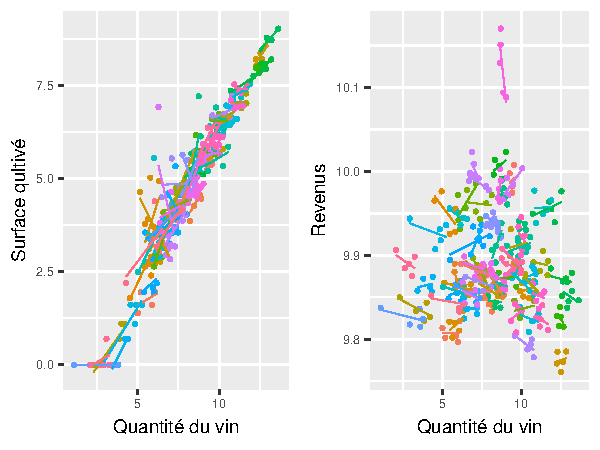
\includegraphics{Presentation_files/figure-beamer/unnamed-chunk-13-1.pdf}

\end{frame}

\begin{frame}{Random and fixed effects testing}
\protect\hypertarget{random-and-fixed-effects-testing}{}

\begin{itemize}
\tightlist
\item
  Poolability tests (tested versus pooled model)
\end{itemize}

\tiny
\begin{table}[!htbp] \centering
  \caption{Effects testing, p-values}
\begin{tabular}{@{\extracolsep{5pt}} l|cc} 
\\[-1.8ex]\hline 
\hline \\[-1.8ex] 
 & Random & Fixed \\ 
\hline \\[-1.8ex] 
Index prix & $0.535$ & $0.533$ \\ 
Index pesticides & $0.485$ & $0.451$ \\ 
Surface & $0$ & $0.0001$ \\ 
Revenus & $0.297$ & $0.247$ \\ 
\hline \\[-1.8ex]
\end{tabular} 
\end{table}

\end{frame}

\begin{frame}{Type of fixed effect testing}
\protect\hypertarget{type-of-fixed-effect-testing}{}

\begin{itemize}
\tightlist
\item
  Type of fixed effects testing
\end{itemize}

\tiny
\begin{table}[!htbp] \centering 
  \caption{Effects testing, p-values}
\begin{tabular}{@{\extracolsep{5pt}} l|ccc} 
\\[-1.8ex]\hline 
\hline \\[-1.8ex] 
 & Individual & Time & Two-ways \\ 
\hline \\[-1.8ex] 
Index prix & $0$ & $0.169$ & $0$ \\ 
Index pesticides & $0$ & $0.222$ & $0$ \\ 
Surface & $0$ & $0.030$ & $0$ \\ 
Revenus & $0$ & $0.248$ & $0$ \\ 
\hline \\[-1.8ex] 
\end{tabular} 
\end{table}

\end{frame}

\begin{frame}{Correlation}
\protect\hypertarget{correlation}{}

\tiny
\begin{table}[!htbp] \centering
  \caption{Overall correlation}
\begin{tabular}{@{\extracolsep{5pt}} l|cccccc}
\\[-1.8ex]\hline
\hline \\[-1.8ex]
 & Quantité du vin & IP & Surface & Revenus & Index pésticides & Temps \\
\hline \\[-1.8ex]
Quantité du vin & $1$ & $0.154$ & $0.956$ & $-0.027$ & $-0.078$ & $-0.036$ \\      
IP & $0.154$ & $1$ & $0.045$ & $-0.037$ & $-0.127$ & $0.043$ \\
Surface & $0.956$ & $0.045$ & $1$ & $-0.057$ & $-0.060$ & $-0.064$ \\
Revenus & $-0.027$ & $-0.037$ & $-0.057$ & $1$ & $-0.052$ & $0.119$ \\
Index pésticides & $-0.078$ & $-0.127$ & $-0.060$ & $-0.052$ & $1$ & $0.291$ \\  
Temps & $-0.036$ & $0.043$ & $-0.064$ & $0.119$ & $0.291$ & $1$ \\
\hline \\[-1.8ex]
\end{tabular}
\end{table}

\end{frame}

\begin{frame}{Modèlisation}
\protect\hypertarget{modelisation}{}

\begin{itemize}
\tightlist
\item
  Explication de la méthode utilisée

  \begin{itemize}
  \tightlist
  \item
    Panel data
  \item
    AIDS model
  \end{itemize}
\item
  Limites du modèle
\end{itemize}

\end{frame}

\begin{frame}{Résultats d'estimation}
\protect\hypertarget{resultats-destimation}{}

\begin{itemize}
\tightlist
\item
  Les coefficients estimés avec leurs variance
\item
  Etude des erreurs
\item
  Vérification des hypothèses (5 hypothèses) :

  \begin{itemize}
  \tightlist
  \item
    La moyenne nulle des herreurs
  \item
    Homoscedacité
  \item
    Autocorrélation
  \item
    Spécification du modèle
  \item
    \ldots{} (à voir)
  \end{itemize}
\end{itemize}

\end{frame}

\begin{frame}{Conclusions}
\protect\hypertarget{conclusions}{}

\begin{itemize}
\tightlist
\item
  Le rôle des pésticides
\item
  Le marché du vin
\item
  Validité
\item
  Limitations
\item
  Ouverture
\end{itemize}

\end{frame}

\begin{frame}{Bibliographie}
\protect\hypertarget{bibliographie}{}

\begin{itemize}
\tightlist
\item
  Inclure seulement les articles importants
\item
  Faire des réferences et mentionner ces articles dans la partie
  théorique
\end{itemize}

\end{frame}

\end{document}
